
\documentclass[doublespace,nopageskip]{VTthesis} % nopageskip = Removes arbitrary blank pages.

%% HPC
\usepackage{latexsym}
\usepackage{graphicx}
\usepackage{mathptmx}
\usepackage{amsmath}
\usepackage{amsfonts}
\usepackage{amssymb}
\usepackage{amsbsy}
\usepackage{amsthm}
\usepackage{float}    % For controlling the placement of tables.
%% 
\usepackage{booktabs} % For formal tables
\usepackage{tikz}     % For drawing example boxes
\usetikzlibrary{positioning}

\usepackage{hyphenat}
\hyphenation{op-tical net-works semi-conduc-tor}

%% Command for creating multiplie-line cells inside a table environment
\newcommand{\multilinecell}[2][c]{%
  \begin{tabular}[#1]{@{}c@{}}#2\end{tabular}}


% Using the following header instead will create a draft copy of your thesis
%\documentclass[doublespace,draft]{VTthesis}

% Title of your thesis
\title{Interpolants and Error Bounds for Modeling and Predicting Variability in Computer Systems}


% You should include 3-5 keywords, separated by commas
\keywords{Approximation Theory, Numerical Analysis, High Performance Computing, Computer Security, Nonparametric Statistics, Mathematical Software}

% Your name, including middle initial(s)
\author{Thomas C. H. Lux}

% Change this to your program, e.g. Physics, Civil Engineering, etc.
\program{Computer Science} 

% Change this to your degree, e.g. Master of Science, Master of Art, etc.
\degree{Doctor of Philosophy} 

% This should be your defense date:
\submitdate{May 16, 2019}

% Committee members. Only have five readers and one chair available.
% Only use the ones you need and don't include the ones you don't need.
% You can also declare a Co-advisor. If you do, the principal and co-advisors
% will be listed as co-advisors on the title page.  Per the VT ETD standards, 
% you should not include titles or educational qualifications such as PhD or Dr.
% You should, however, include middle initials if possible.
\principaladvisor{Layne Watson}
\coadvisor{Yili Hong}
\firstreader{Kirk Cameron}
\secondreader{Bert Huang}
\thirdreader{Gang Wang}
\fourthreader{Yang Cao}

% The dedication and acknowledgement pages are optional. Comment them out to remove them.
%% \dedication{...}
%% \acknowledge{...}

% The abstract is required and should be <=250 words for thesis, <=350 words for dissertation.
\abstract{Function approximation is an important problem. This work presents applications of interpolants to modeling random variables. Specifically, this work studies the prediction of distributions of random variables applied to computer system throughput variability. New methods for interpolating data with moderately high dimension are presented and novel theoretical error bounds are constructed for piecewise linear interpolation. Finally, a mathematical software for approximating distributions from data samples via monotone quintic splines is proposed.}

% The general audience abstract is required. There are currently no word limits.
\abstractgenaud{It is common for scientists to collect data on something they are studying. Often scientists want to create a (predictive) model of that phenomenon based on the data, but the choice of \textit{how} to model the data is a difficult one to answer. This work proposes methods for modeling data that operate under very few assumptions that are broadly applicable across science. Finally, a software package is proposed that would allow scientists to better understand the \textit{true} distribution of their data given relatively few observations.}

\begin{document}
% The following lines set up the front matter of your thesis or dissertation and is required to ensure proper formatting per the VT ETD standards. 
\frontmatter
\maketitle
\tableofcontents

% The list of figures and tables are now optional per the official ETD standards.  Unless you have a very good reason for removing them, you should leave these lists in the document. Comment them out to remove them.
\listoffigures
\listoftables

%% \printnomenclature %creates a list of abbreviations. Comment out to remove it. 
%% ABBR is described here.
%% \nomenclature{ABBR}{abbreviation}

% The following sets up the document for the main part of the thesis or dissertation. Do not comment out or remove this line.
\mainmatter


%% Introduction of variability modeling, the importance of modeling in science in general, then dive into the specific application of modeling techniques to systems (and security).
\chapter{The Importance and Applications of Variability} \label{ch:apps}

Computational variability presents itself in a variety of forms. Processes that are apparently identical in a cloud computing or high performance computing (HPC) environment may take different amounts of time to complete the same job. This variability can cause unintentional violations of service level agreements in cloud computing applications or indicate suboptimal performance in HPC applications. The sources of variability, however, are distributed throughout the system stack and often difficult to identify. The methodology presented in this work is applicable to modeling the expected variability of useful computer system performance measures without any prior knowledge of system architecture. Some examples of interesting performance measures that could be modeled with the techniques in this work include computational throughput, power consumption, processor idle time, number of context switches, and RAM usage, as well as any other numeric measure of performance.

Predicting performance variability in a computer system is a challenging problem that has primarily been attempted in one of two ways: (1) build a statistical model of the performance data collected by running experiments on the system at select settings, or (2) run artificial experiments using a simplified simulation of the target system to estimate architecture and application bottlenecks. In this work, modeling techniques rest in the first category and represent a notable increase in the ability to model precise characteristics of variability.

Many previous works attempting to model system performance have used simulated environments \cite{grobelny2007fase,wang2009simulation,wang2013towards}. \citet{grobelny2007fase} refer to statistical models as being oversimplified and not capable of capturing the true complexity of the underlying system. Historically, statistical models have been limited to modelling at most one or two system parameters and have therefore not been capable of modeling the complexity of the underlying system \cite{snavely2002framework,bailey2005performance,barker2009using,ye2010analyzing}. These limited statistical models have provided satisfactory performance in narrow application settings. However these techniques require additional code annotations, hardware abstractions, or additional assumptions about the behavior of the application in order to generate models. In contrast, the approaches that are presented here require no modifications of applications, no architectural abstractions, nor any structural descriptions of the input data being modeled. The techniques used in this work only require performance data as input.

Most existing work on performance variability has focused on operating system (OS) induced variability \cite{beckman2008benchmarking,de2007identifying}. Yet, system I/O variability has been particularly difficult for statistical models to capture \cite{bailey2005performance}. The prior work attempting to model I/O variability has been similarly limited to one or two system parameters \cite{lofstead2010managing}.

Chapters \ref{ch:naive} and \ref{ch:strong} present and evaluate applications of multivariate interpolation to the domain of computer system I/O throughput. Interpolants and regressors are used to predict the different measures of variability (e.g., mean, variance, cumulative distribution functions) for the expected I/O throughput on a system with previously unseen configurations. Beyond these I/O case studies, the techniques discussed can tractably model tens of interacting system parameters with tens of thousands of known configurations. A major contribution of this work is a modeling framework that uses multivariate interpolation to capture precise characteristics (via cumulative distribution functions) of arbitrary performance measure on any type of computer system.


\section{Broader Applications of Approximation}

Regression and interpolation are problems of considerable importance
that find applications across many fields of science. Pollution and
air quality analysis \cite{de2008field}, energy consumption management
\cite{lazos2014optimisation}, and student performance prediction
\cite{cortez2008using,lux2016applications} are a few of many
interdisciplinary applications of multivariate regression for
predictive analysis. As discussed later, these techniques can also be
applied to prediction problems related to forest fire risk assessment
\cite{cortez2007data}, Parkinson's patient clinical evaluations
\cite{tsanas2010accurate}, local rainfall and weather
\cite{williams2009rattle}, credit card transactions
\cite{pozzolo2015calibrating}, and high performance computing (HPC)
file input/output (I/O) \cite{lux2018nonparametric}.

Regression and interpolation have a considerable theoretical base in
one dimension \cite{cheney2009course}. Splines in particular are well
understood as an interpolation technique in one dimension
\cite{de1978practical}, particularly B-splines. Tensor products of
B-splines \cite{unther1996interpolating} or other basis functions have
an unfortunate exponential scaling with increasing
dimension. Exponential scaling prohibits tensor products from being
reasonably applied beyond three-dimensional data. In order to address
this dimensional scaling challenge, C. de Boor and others proposed box
splines \cite{de2013box}, of which one of the approximation techniques
in Chapter \ref{ch:boxes} of this work is composed \cite{lux2018novel}.

The theoretical foundation of low dimensional interpolation allows the
construction of strong error bounds that are absent from high
dimensional problems. Chapter \ref{ch:error} extends some known
results regarding the secant method \cite{dennis1996numerical} to
construct an interpolation error bound for problems of arbitrary
dimension. These error bounds are useful, considering the same cannot
be said for regression algorithms in general. The maximum complexity
of an interpolant is bounded by the amount of data available, while
the maximum complexity of a regressor is bounded by both the amount of
data and the chosen parametric form. For this reason, generic uniform
bounds are largely unobtainable for regression techniques on arbitrary
approximation problems, even when the approximation domain is
bounded. These generic bounds imply that interpolants may be suitable
for a broader class of approximation problems than (heuristically
chosen) regression techniques.

Aside from theoretical motivation for the use of interpolants, there
are often computational advantages as well. Interpolants do not have
the need for \textit{fitting} data, or minimizing error with respect
to model parameters. In applications where the amount of data is large
and the relative number of predictions that need to be made for a
given collection of data is small, the direct application of an
interpolant is much less computationally expensive.

In this work, multivariate interpolation is defined given a closed
convex subset $Y$ of a metrizable topological vector space with metric
$s$, some function $f:\mathbb{R}^d \rightarrow Y$ and a set of points
$X = \bigl\{x^{(1)}$, $\ldots$, $x^{(n)}\bigr\} \subset \mathbb{R}^d$,
along with associated function values $f\bigl(x^{(i)}\bigr)$. The goal
is to construct an approximation $\hat f: \mathbb{R}^d \rightarrow Y$
such that $\hat f\bigl(x^{(i)}\bigr) = f\bigl(x^{(i)}\bigr)$ for all
$i = 1$, $\ldots$, $n$. It is often the case that the form of the true
underlying function $f$ is unknown, however it is still desirable to
construct an approximation $\hat f$ with small approximation error at
$y \notin X$. The two metric spaces that will be discussed in this
work are the real numbers with metric $s(x,y) = |x-y|$, and the set of
cumulative distribution functions (CDFs) with the Kolmogorov-Smirnov
(KS) statistic \cite{lilliefors1967kolmogorov} as metric.

Multivariate regression is often used when the underlying function is
presumed to be stochastic, or stochastic error is introduced in the
evaluation of $f$. Hence, multivariate regression relaxes the
conditions of interpolation by choosing parameters $P$ defining $\hat
f(x;P)$ to minimize the error vector $\Bigl( \bigl | \hat f
\bigl(x^{(1)};P\bigr) - f\bigl(x^{(1)}\bigr) \bigr|$, $\ldots$, $\bigl
| \hat f \bigl(x^{(n)}; P\bigr) - f\bigl(x^{(n)}\bigr) \bigr | \Bigr)$
in some norm. The difficult question in the case of regression is
often what parametric form to adopt for any given application.

The most challenging problem when scaling in dimension is that the
number of possible interactions between dimensions grows
exponentially. Quantifying all possible interactions becomes
intractable, and hence beyond three-dimensional data mostly linear
models are used. That is not to say nonlinear models are absent, but
nonlinearities are often either preconceived or model pairwise
interactions between dimensions at most. Even globally nonlinear
approximations such as neural networks are constructed from
compositions of summed low-interaction functions
\cite{clevert2015fast}.

Provided the theoretical and practical motivations for exploring
interpolants, this work aims to study the empirical performance
differences between a set of scalable (moderately) interpolation
techniques and a set of common regression techniques. These techniques
are applied to a collection of moderately high dimensional problems
($5 \le d \le 30$) and the empirical results are discussed.

\section{An Initial Application of Approximation}

Performance tuning is often an experimentally complex and time
intensive chore necessary for configuring High Performance Computing
(HPC) systems. The procedures for this tuning vary largely from system
to system and are often subjectively guided by the system
engineer(s). Once a desired level of performance is achieved, an HPC
system may only be incrementally reconfigured as required by updates
or specific jobs. In the case that a system has changing workloads or
nonstationary performance objectives that range from maximizing
computational throughput to minimizing power consumption and system
variability, it becomes clear that a more effective and automated tool
is needed for configuring systems. This scenario presents a
challenging and important application of multivariate approximation
and interpolation techniques.

Among the statistical models presented in prior works for modeling computer systems,
\cite{bailey2005performance} specifically mention that it is difficult
for simplified models to capture variability introduced by
I/O. System variability in general has become a problem of increasing
interest to the HPC and systems communities, however most of the work
has focused on operating system (OS) induced variability
\cite{beckman2008benchmarking,de2007identifying}. The work that has
focused on managing I/O variability does not use any sophisticated
modeling techniques \cite{lofstead2010managing}. Hence, Chapter
\ref{ch:naive} presents a case study applying advanced mathematical
and statistical modeling techniques to the domain of HPC I/O
characteristics. The models are used to predict the mean throughput of
a system and the variance in throughput of a system. The discussion
section that follows outlines how the techniques presented can be
applied to any performance metric and any system.


%% Describe all of the interpolants and regressors that will be used throughout this work. (except meshes)
\chapter{Algorithms for Constructing Approximations} \label{ch:algs}
%% ===================================================================
\section{Multivariate Regression}
\label{sec:regression}
Multivariate regressors are capable of accurately modeling a complex
dependence of a response (in $Y$) on multiple variables (represented
as a points in $\mathbb{R}^{d}$). The approximations to some (unknown)
underlying function $f: \mathbb{R}^d \rightarrow Y$ are chosen to
minimize some error measure related to data samples
$f\bigl(x^{(i)}\bigr)$. For example, least squares regression uses the
sum of squared differences between modeled function values and true
function values as an error measure. In this section and the next,
some techniques are limited to approximating real valued functions ($Y
\subset \mathbb{R}$). These techniques can be extended to real
vector-valued ranges by repeating the construction for each component
of the vector output. Throughout the following, $x$ denotes a
$d$-tuple, $x_i$ the $i$th component of $x$, and $x^{(i)}$ the $i$th
$d$-tuple data point. Different symbols are used to represent the
approximation function $\hat f$.

\subsection{Multivariate Adaptive Regression Splines}
\label{sec:mars}
This approximation was introduced in \cite{friedman1991multivariate}
and subsequently improved to its current version in
\cite{stanford1993fast}, called fast multivariate adaptive regression
splines (Fast MARS). In Fast MARS, a least squares fit model is
iteratively built by beginning with a single constant valued function
and adding two new basis functions at each iteration of the form
\begin{align*}
  B_{2j-1}(x) &= B_l(x) \bigl(x_i-x^{(p)}_i\bigr)_+, \\
  B_{2j}(x) &= B_k(x) \bigl(x_i-x^{(p)}_i\bigr)_- ,
\end{align*}
where $j \leq m$ is the iteration number, $m$ is the maximum
  number of underlying basis functions, $1 \le p \le n$, and
$B_l(x)$, $B_k(x)$ are basis functions from the previous iteration,
 $$w_+ = \begin{cases} w, & w \geq 0 \\ 0, & w < 0 \end{cases},$$ and
$w_- = (-w)_+$. After iteratively constructing a model, MARS then
iteratively removes basis functions that do not contribute to goodness
of fit. In effect, MARS creates a locally component-wise tensor
product approximation of the data. The overall computational
complexity of Fast MARS is $\mathcal{O}(n d m^3)$. This paper
uses an implementation of Fast MARS \cite{rudy2017pyearth} with $m =
200$ throughout all experiments.

\subsection{Support Vector Regressor}
\label{sec:svr}
Support vector machines are a common method used in machine learning
classification tasks that can be adapted for the purpose of regression
\cite{basak2007support}. How to build a support vector regressor (SVR)
is beyond the scope of this summary, but the resulting functional fit
$p : \mathbb{R}^d \rightarrow \mathbb{R}$ has the form
 $$ p(x)  = \sum_{i=1}^{n}a_i K\bigl(x,x^{(i)}\bigr) + b ,$$
where $K$ is the selected kernel function, $a_i \in \mathbb{R}^n$, 
$b \in \mathbb{R}$ are coefficients to be solved for simultaneously.
The computational complexity of the SVR is $\mathcal{O}(n^2dm)$, with
$m$ being determined by the minimization convergence criterion. This
paper uses the scikit-learn SVR \cite{scikit-learn} with a radial
basis function kernel.

\subsection{Multilayer Perceptron Regressor}
\label{sec:mlp}
The neural network is a well studied and widely used method for both
regression and classification tasks
\cite{hornik1989multilayer,rumelhart1988learning}. When using the
rectified linear unit (ReLU) activation function
\cite{dahl2013improving} and fitting the model with stochastic
gradient descent (SGD) or BFGS minimization techniques
\cite{goh2017why,moller1993scaled,robbins1951stochastic}, the model
built by a multilayer perceptron uses layers $l : \mathbb{R}^{i}
\rightarrow \mathbb{R}^{j}$ defined by
 $$ l(u) = \bigl( u^t W_l + c_l \bigr)_+ ,$$
where $c_l \in \mathbb{R}^j$ and $W_l$ is the $i \times j$ weight
matrix for layer $l$. In this form, the multilayer perceptron (MLP)
produces a piecewise linear model of the input data. The computational
complexity of training a multilayer perceptron is $\mathcal{O}(n d
m)$, where $m$ is determined by the sizes of the layers of the network
and the stopping criterion of the minimization used for finding
weights. This paper uses an MLP built from Keras and Tensorflow to
perform regression \cite{tensorflow2015-whitepaper,chollet2015keras}
with ten hidden layers each having thirty two nodes (a total of
approximately ten thousand parameters), ReLU activation, and
one hundred thousand steps of SGD
for training. It should be noted that the choice of neural
  network architecture affects approximation performance, but no
  architecture tuning is performed here.

%% ===================================================================
\section{Multivariate Interpolation}
\label{sec:interpolation}
The following interpolation techniques demonstrate a reasonable
variety of approaches to interpolation. All of the presented
interpolants produce approximations that are continuous in value,
which is often a desirable property in applied approximation problems.

\subsection{Delaunay}
\label{sec:delaunay}

The Delaunay triangulation is a well-studied geometric technique for
producing an interpolant \cite{lee1980two}. The Delaunay triangulation
of a set of points into simplices is such that there
are no points inside the sphere defined by the
vertices of each simplex. For a $d$-simplex S with vertices $x^{(0)}$,
$x^{(1)}$, $\ldots$, $x^{(d)}$, and function values
$f\bigl(x^{(i)}\bigr)$, $i=0$, $\ldots$, $d$, $y \in S$ is a unique
convex combination of the vertices,
 $$ y = \sum_{i=0}^{d} w_i x^{(i)}, \quad \sum_{i=0}^{d} w_i = 1, \quad w_i \geq 0, \quad i=0,\ldots,d, $$
and the Delaunay interpolant $\hat f(y)$ at $y$ is given by
 $$ \hat f(y) = \sum_{i=0}^{d} w_i f\bigl(x^{(i)}\bigr). $$ The
computational complexity of Delaunay interpolation (for the
implementation used \cite{chang2018polynomial}) is $\mathcal{O}(k n
d^3)$. Given pathological data the entire triangulation could be
computed with $k = n^{\lceil d / 2 \rceil}$, but the average case yields
$k = d \log d$ and is capable of scaling reasonably to $d \leq 50$. In
the present application, a Delaunay simplex $S$ containing $y$ is
found, then the $d+1$ vertices (points in $X$) of $S$ are used to
assign weights to each vertex and produce the predicted function value
for point $y$.

\begin{figure}
  \centering
  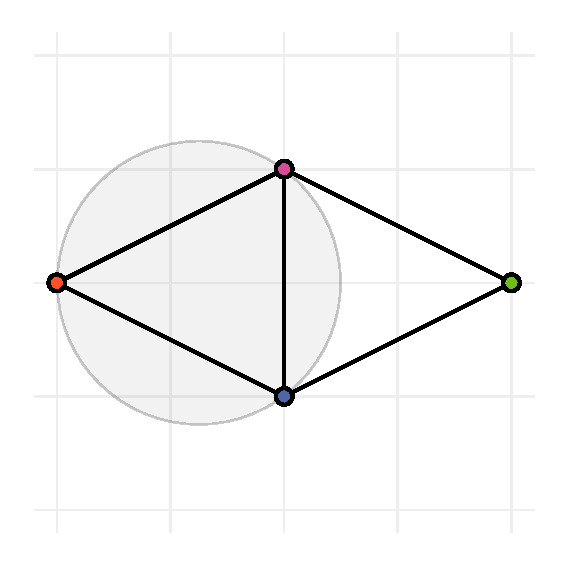
\includegraphics[width=0.4\textwidth,]{Figures/NA/example_delaunay.pdf}
  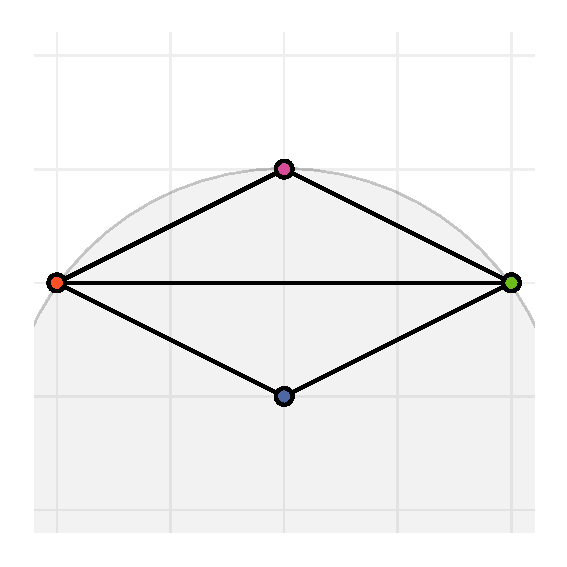
\includegraphics[width=0.4\textwidth,]{Figures/NA/example_not_delaunay.pdf}
  \caption{On the left above is a depiction of a Delaunay
    triangulation over four points, notice that the circumball (shaded
    circle) for the left simplex does not contain the fourth point.
    On the right above, a non-Delaunay mesh is depicted. Notice that
    the circumball for the top simplex (shaded circle, clipped at
    bottom edge of the visual) contains the fourth point which
    violates the Delaunay condition for a simplex.
  \vspace{-.1cm}}
  \label{fig:delaunay}
\end{figure}


\subsection{Modified Shepard}
\label{sec:modified-shepard}

The modified Shepard method used here (ShepMod) generates a continuous
approximation based on Euclidean distance and resembles a nearest
neighbor interpolant \cite{cover1967nearest}. This model is a type of
\textit{metric interpolation}, also called a Shepard method
\cite{gordon1978shepard,shepard1968two}. The interpolant has the form
 $$ p(x) = \frac{\sum\limits_{k=1}^{n}W_k(x)f\bigl(x^{(k)}\bigr)}
     {\sum\limits_{k=1}^{n}W_k(x)} ,$$ where
     $p\bigl(x^{(k)}\bigr) = f\bigl(x^{(k)}\bigr)$, $W_k(x) =
       \bigl(\bigl(r_k - \bigl\|x - x^{(k)}\bigr\|_2\bigr)_+ \big/
       \bigl( r_k \bigl\|x - x^{(k)}\bigr\|_2 \bigr)\bigr)^2$ for $x
       \neq x^{(k)}$, and $r_k \in \mathbb{R}$ is the smallest
     radius such that at least $d+1$ other points $x^{(j)}$, $j \not =
     k$, are inside the closed Euclidean ball of radius $r_k$ about
     $x^{(k)}$. The interpolant $p(x)$ is continuous because
       the singularities at the $x^{(k)}$ are removable. The
     computational complexity of ShepMod is $\mathcal{O}(n^2d)$. This
     paper uses a Fortran 95 implementation of ShepMod derived from
     SHEPPACK \cite{thacker2010algorithm}.

\begin{figure}
  \centering
  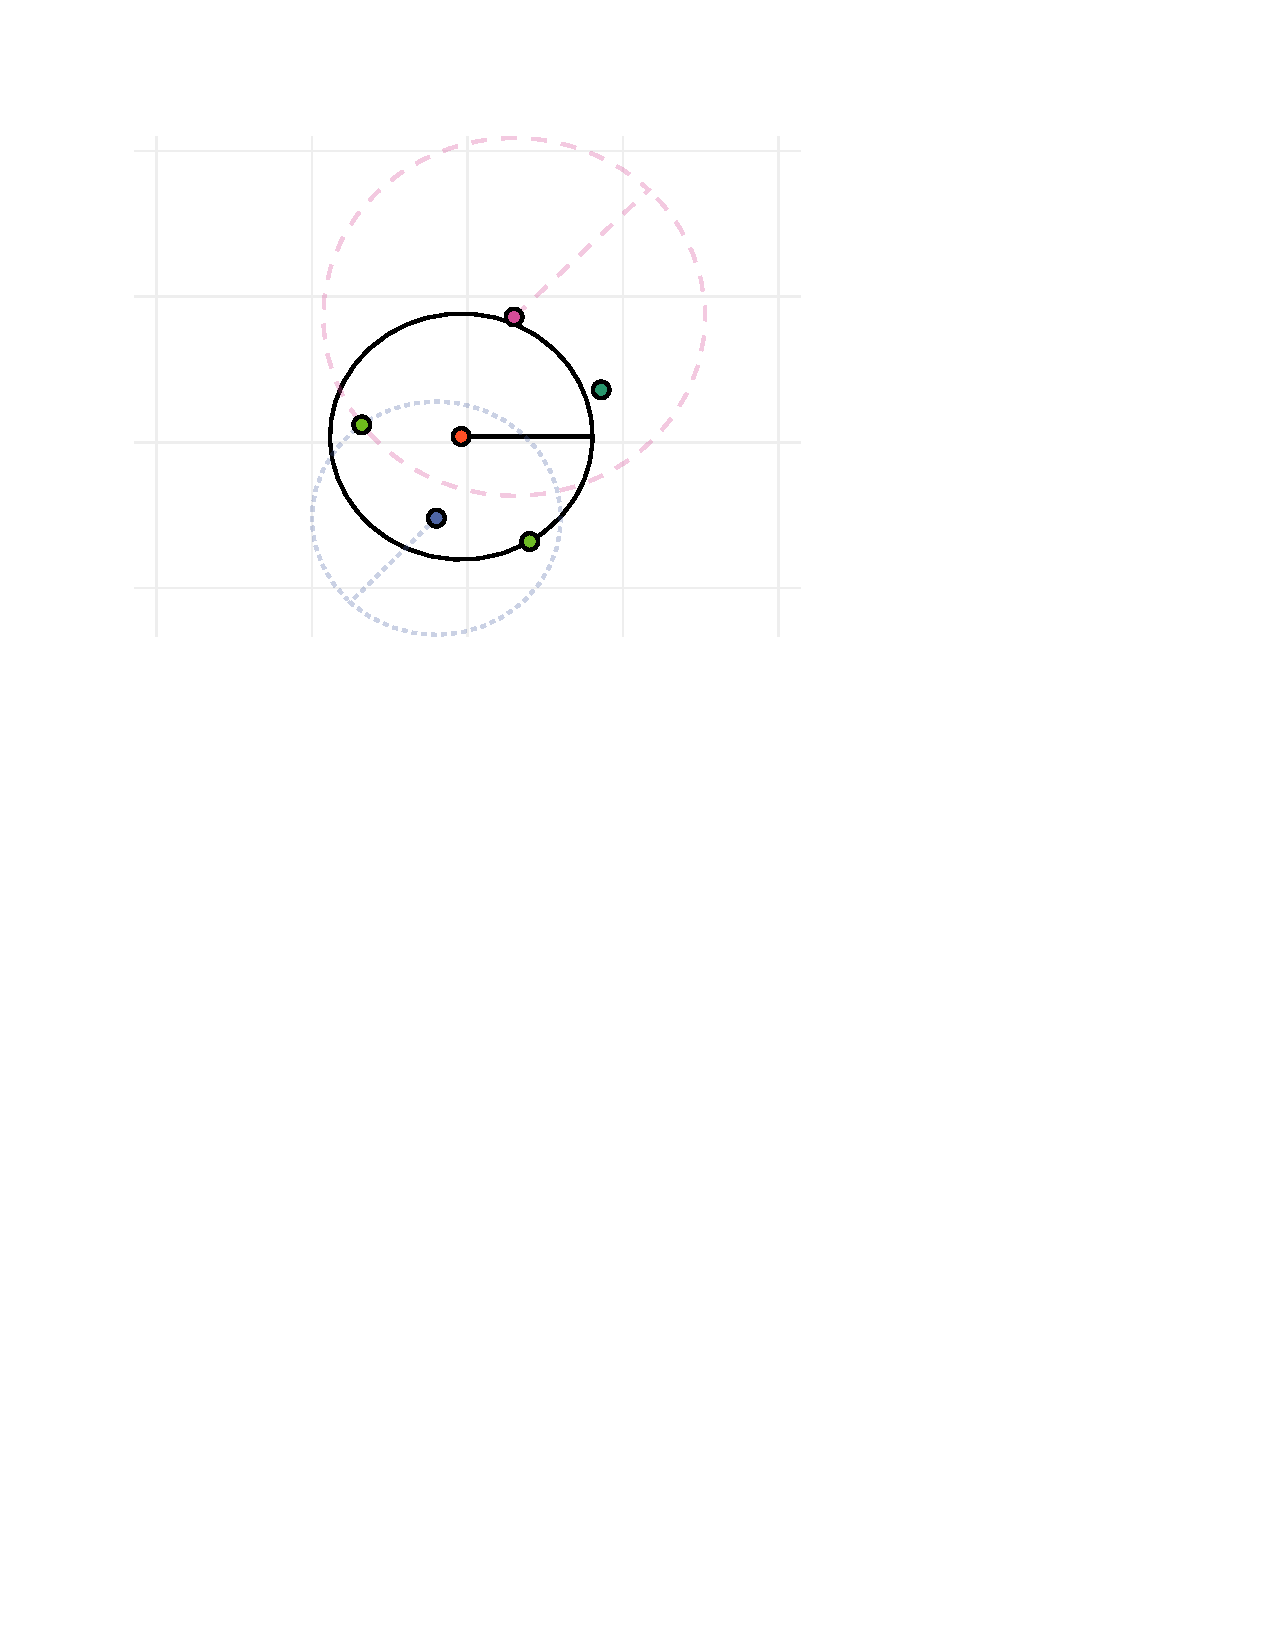
\includegraphics[width=0.4\textwidth,]{Figures/NA/example_shepard_radius.pdf}
  \hspace{.2cm}
  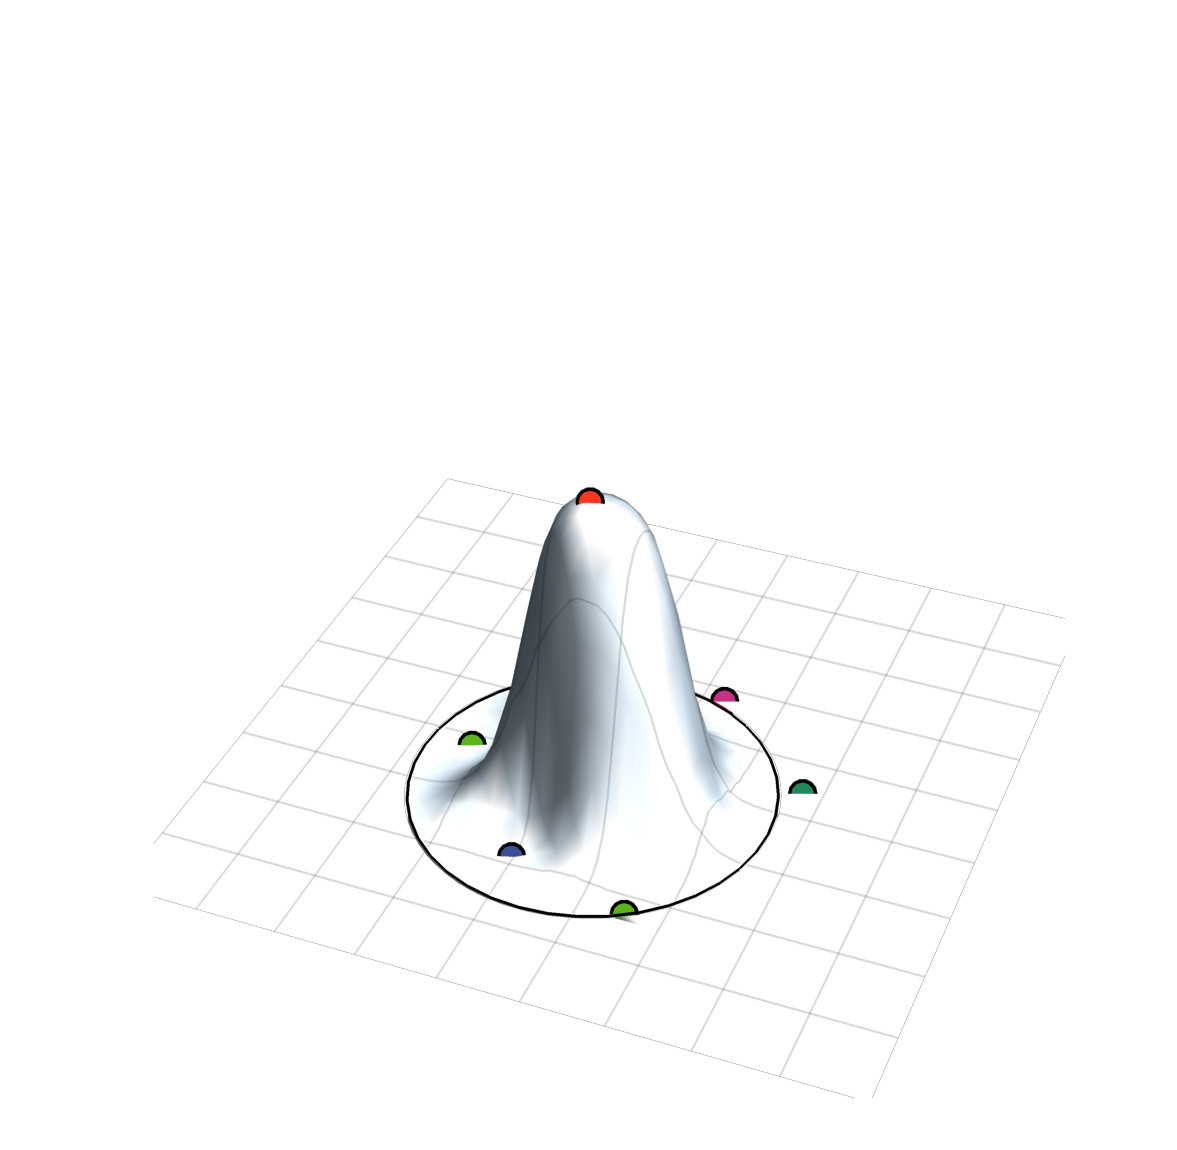
\includegraphics[width=0.4\textwidth,]{Figures/NA/example_shepard_weight.pdf}
  \caption{On the left above is a depiction of the radius
    of influence for three chosen points of a collection in two
    dimensions using the modified Shepard criteria. On the right a
    third axis shows the relative weight for the center most
    interpolation point $x^{(i)}$ with the solid line representing its
    radius of influence, where $W_i(x)$ is $0$ for $\|x-x^{(i)}\|_2
    \geq r_i$ and $W_i(x) / \sum_{k=1}^n W_k(x) \to 1$ as $x \to
    x^{(i)}$.
  \vspace{-.1cm}}
  \label{fig:shepard}
\end{figure}


\subsection{Linear Shepard}
The linear Shepard method (LSHEP) is a blending function using local
linear interpolants, a special case of the general Shepard algorithm
\cite{thacker2010algorithm}. The interpolant has the form
 $$ p(x) = \frac{\sum\limits_{k=1}^{n}W_k(x)P_k(x)}
 {\sum\limits_{k=1}^{n}W_k(x)} ,$$
where $W_k(x)$ is the same as for the modified Shepard method and
$P_k(x)$ is a local linear approximation to the data satisfying
$P_k\bigl(x^{(k)}\bigr) = f\bigl(x^{(x)}\bigr)$. The computational
complexity of LSHEP is $\mathcal{O}(n^2d^3)$. This paper uses the
Fortran 95 implementation of LSHEP in SHEPPACK
\cite{thacker2010algorithm}.


%% Demonstrate the naive application of interpolants and regressors to data. Discuss results.
\chapter{Na\"{\i}ve Approximations of Variability} \label{ch:naive}

This chapter compares five of the multivariate approximation
techniques that operate on inputs in $\mathbb{R}^d$ ($d$-tuples of
real numbers) and produce predicted responses in $\mathbb{R}$. Three
of the chosen techniques are regression based and the remaining two
are interpolants, providing reasonable coverage of the varied
mathematical strategies that can be employed to solve continuous
modeling problems.

%     Methodology     
%=====================
\section{I/O Data}

In order to evaluate the viability of multivariate models for
predicting system performance, this paper presents a case study of a
four-dimensional dataset produced by executing the IOzone benchmark
from \citet{iozone} on a homogeneous cluster of computers. Multiple
I/O Zone data sets will be used throughout the work, however this
chapter relies on this specific four-dimensional dataset. All
experiments were performed on parallel shared-memory nodes common to
HPC systems. Each system had a lone guest Linux operating system
(Ubuntu 14.04 LTS//XEN 4.0) on a dedicated 2TB HDD on a 2 socket, 4
core (2 hyperthreads per core) Intel Xeon E5-2623 v3 (Haswell)
platform with 32 GB DDR4. The system performance data was collected by
executing IOzone 40 times for each of a select set of system
configurations. A single IOzone execution reports the max I/O
throughput seen for the selected test in kilobytes per second. The 40
executions for each system configuration are converted into the mean
and variance, both values in $\mathbb{R}$ capable of being modeled
individually by the multivariate approximation techniques presented in
Chapter \ref{ch:algs}. The summary of data used in the experiments for
this chapter can be seen in Table \ref{tab:data_type}.  Distributions
of raw throughput values being modeled can be seen in Figure
\ref{fig:raw_throughput}.

\begin{table}
  \centering
  \begin{tabular}{c|c}
    \hline
    \textbf{System Parameter} & \textbf{Values}\\
    \hline
    File Size & 64, 256, 1024\\
    Record Size & 32, 128, 512\\
    Thread Count & 1, 2, 4, 8, 16, 32, 64, 128, 256\\
    Frequency & \{12, 14, 15, 16, 18, 19, 20, 21, 23, 24, 25, 27, 28, 29, 30, 30.01\} $\times 10^5$\\
    \hline
    \textbf{Response Values} & \\
    \hline
    Throughput Mean & [$2.6 \times 10^5$, $5.9 \times 10^8$]\\
    Throughput Variance & [$5.9\times 10^{10} $, $4.7 \times 10^{16}$]\\
    \hline
  \end{tabular}
  \caption{A description of the system parameters being considered in
    the IOzone tests. Record size must not be greater than file size
    and hence there are only six valid combinations of the two. In
    total there are $6 \times 9 \times 16 = 864$ unique system
    configurations.}
  \label{tab:data_type}
\end{table}

\begin{figure}
  \centering
  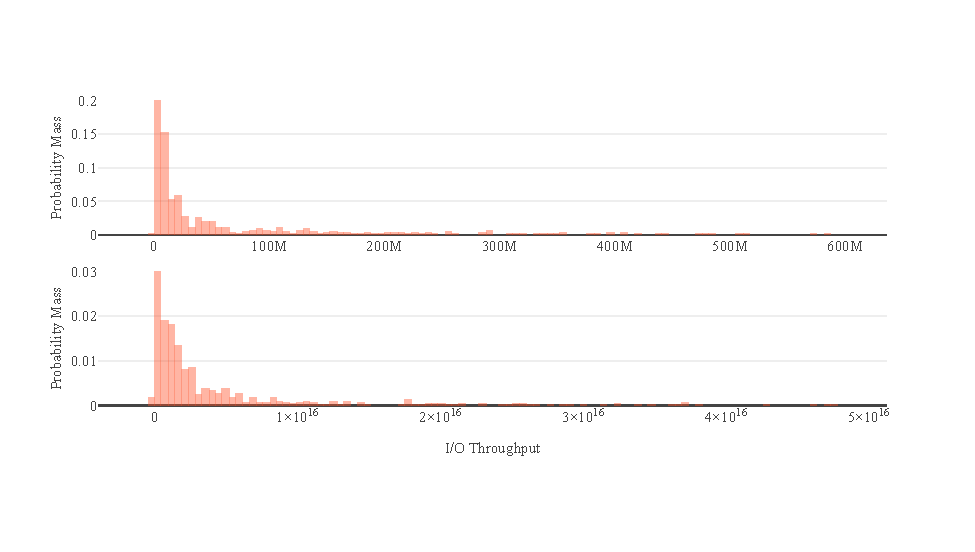
\includegraphics[width=\textwidth,trim={0 .5in 0 .4in}]{Figures/HPC/Raw_Throughput.pdf}
  \caption{Histograms of 100-bin reductions of the PMF of I/O
    throughput mean (top) and I/O throughput variance (bottom). In the
    mean plot, the first 1\% bin (truncated in plot) has a probability
    mass of .45. In the variance plot, the second 1\% bin has a
    probability mass of .58. It can be seen that the distributions of
    throughputs are primarily of lower magnitude with occasional
    extreme outliers.}
  \label{fig:raw_throughput}
\end{figure}

\subsection{Dimensional Analysis}

This analysis utilizes an extension to standard $k$-fold cross
validation that allows for a more thorough investigation of the
expected model performance in a variety of real-world
situations. Alongside randomized splits, two extra components are
considered: the amount of training data provided, and the dimension of
the input data. It is important to consider that algorithms that
perform well with less training input also require less
experimentation. Although, the amount of training data required may
change as a function of the dimension of the input and this needs to
be studied as well. The framework used here will be referred to as a
multidimensional analysis (MDA) of the IOzone data.

\subsubsection{Multidimensional Analysis}

This procedure combines random selection of training and testing
splits with changes in the input dimension and the ratio of training
size to testing size. Given an input data matrix with $n$ rows
(points) and $d$ columns (components), MDA proceeds as follows:
\begin{enumerate}
\item For all $k = 1$, $\ldots$, $d$ and for all nonempty subsets $F
  \subset \{1, 2, \ldots, d\}$, reduce the input data to points $(z,
  f_F(z))$ with $z \in \mathbb{R}^k$ and $f_F(z) = E\bigl[ \bigl\{
    f\bigl(x^{(i)}\bigr) \bigm| \bigl(x^{(i)}_F = z\bigr) \bigr\}
    \bigr]$, where $E[\cdot]$ denotes the mean and $x^{(i)}_F$ is the
  subvector of $x^{(i)}$ indexed by $F$.
\item For all $r$ in $\{5, 10, \ldots, 95\}$, generate $N$ random
  splits $(train, test)$ of the reduced data with $r$ percentage for
  training and $100 - r$ percentage for testing.
\item When generating each of $N$ random $(train, test)$ splits,
  ensure that all points from $test$ are in the convex hull of points
  in $train$ (to prevent extrapolation); also ensure that the points
  in $train$ are well spaced.
\end{enumerate}

In order to ensure that the testing points are in the convex hull of
the training points, the convex hull vertices of each set of (reduced
dimension) points are forcibly placed in the training set. In order to
ensure that training points are well spaced, a statistical method for
picking points from \citet{amos2014algorithm} is used:
\begin{enumerate}
\item Generate a sequence of all pairs of points
  $\bigl(z^{(i_1)},z^{(j_1)}\bigr), \bigl(z^{(i_2)},z^{(j_2)}\bigr),
  \ldots$ sorted by ascending pairwise Euclidean distance between
  points, so that $\bigl|\bigl|z^{(i_k)}-z^{(j_k)}\bigr|\bigr|_2 \leq
  \bigl|\bigl|z^{(i_{k+1})}-z^{(j_{k+1})}\bigr|\bigr|_2$.
\item Sequentially remove points from candidacy until only $|train|$
  remain by randomly selecting one point from the pair
  $\bigl(z^{(i_m)}, z^{(j_m)}\bigr)$ for $m = 1,\ldots$ if both
  $z^{(i_m)}$ and $z^{(j_m)}$ are still candidates for removal.
\end{enumerate}

Given the large number of constraints, level of reduction, and use of
randomness in the MDA procedure, occasionally $N$ unique
training/testing splits may not be created or may not exist. In these
cases, if there are fewer than $N$ possible splits, then
deterministically generated splits are used. Otherwise after $3N$
attempts, only the unique splits are kept for analysis. The MDA
procedure has been implemented in Python\#3 while most regression and
interpolation methods are Fortran wrapped with Python. All randomness
has been seeded for repeatability.

For any index subset $F$ (of size $k$) and selected value of $r$, MDA
will generate up to $N$ multivariate models $f_F(z)$ and predictions
$\hat{f}_F\big(z^{(i)}\big)$ for a point $z^{(i)} \in \mathbb{R}^k$.
There may be fewer than $N$ predictions made for any given
point. Extreme points of the convex hull for the selected index subset
will always be used for training, never for testing. Points that do
not have any close neighbors will often be used for training in order
to ensure well-spacing. Finally, as mentioned before, some index
subsets do not readily generate $N$ unique training and testing
splits. The summary results presented in this work use the median of
the ($N$ or fewer) values $\hat{f}_F(z)$ at each point as the model
estimate for error analysis.


\section{Na\"{\i}ve Variability Modeling Results}

A na\"{\i}ve multivariate prediction technique such as nearest
neighbor could experience relative errors in the range $\displaystyle
[0, \big(\max_x f(x) - \min_x f(x)\big) / \min_x f(x) ]$ when modeling
a nonnegative function $f(x)$ from data. The IOzone mean data response
values span three orders of magnitude (as can be seen in Table
\ref{tab:data_type}) while variance data response values span six
orders of magnitude. It is expected therefore, that all studied
multivariate models perform better than a na\"{\i}ve approach,
achieving relative errors strictly less than $10^3$ for throughput
mean and $10^6$ for throughput variance. Ideally, models will yield
relative errors significantly smaller than 1. The time required to
compute thousands of models involved in processing the IOzone data
through MDA was approximately five hours on a CentOS workstation with
an Intel i7-3770 CPU at 3.40GHz. In four dimensions for example, each
of the models could be constructed and evaluated over hundreds of
points in less than a few seconds.


\subsection{I/O Throughput Mean}

Almost all multivariate models analyzed make predictions with a
relative error less than 1 for most system configurations when
predicting the mean I/O throughput of a system given varying amounts
of training data. The overall best of the multivariate models,
Delaunay, consistently makes predictions with relative error less than
$.05$ (5\% error). In Figure \ref{fig:mean_tt_ratio} it can also be
seen that the Delaunay model consistently makes good predictions even
with as low as 5\% training data (43 of the 864 system configurations)
regardless of the dimension of the data.

\begin{figure}
  \centering
  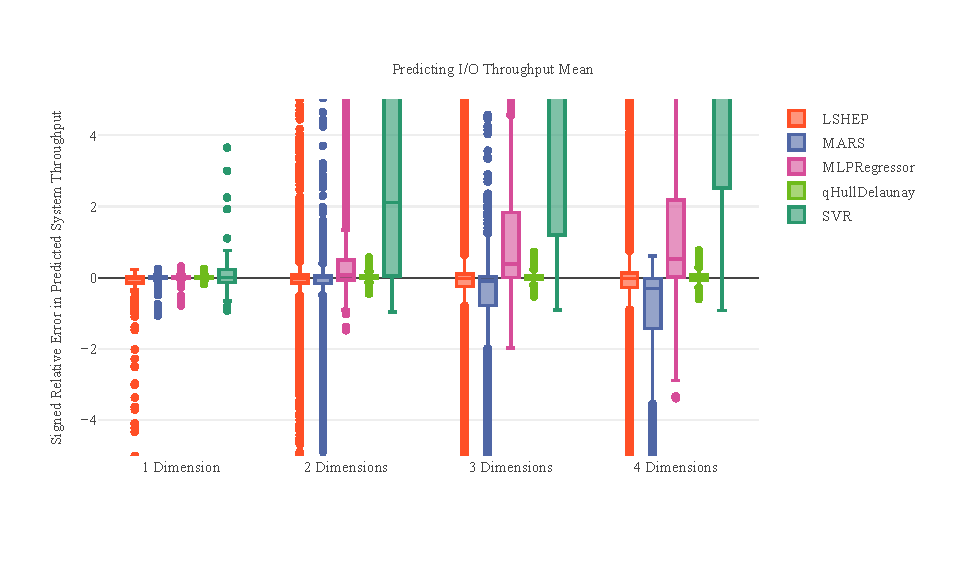
\includegraphics[width=\textwidth,trim={0 .5in 0 .3in}]{Figures/HPC/Mean_Dim.pdf}
  \caption{These box plots show the prediction error of mean with
    increasing dimension. The top box whisker for SVR is 40, 80, 90
    for dimensions 2, 3, and 4, respectively. Notice that each model
    consistently experiences greater magnitude error with increasing
    dimension. Results for all training percentages are aggregated.}
  \label{fig:mean_dim}
\end{figure}

\begin{figure}
  \centering
  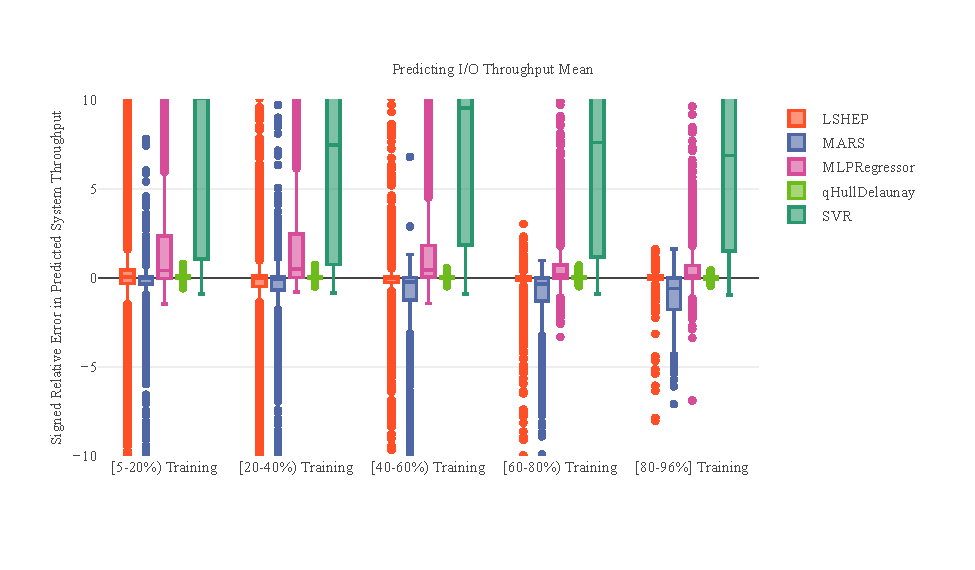
\includegraphics[width=\textwidth,trim={0 .5in 0 .3in}]{Figures/HPC/Mean_TT_Ratio.pdf}
  \caption{These box plots show the prediction error of mean with
    increasing amounts of training data provided to the models. Notice
    that MARS is the only model whose primary spread of performance
    increases with more training data. Recall that the response values
    being predicted span three orders of magnitude and hence relative
    errors should certainly remain within that range. For SVR the top
    box whisker goes from around 100 to 50 from left to right and is
    truncated in order to maintain focus on better models. Results for
    all dimensions are aggregated. Max training percentage is 96\% due
    to rounding training set size.}
  \label{fig:mean_tt_ratio}
\end{figure}

\begin{figure}
  \centering
  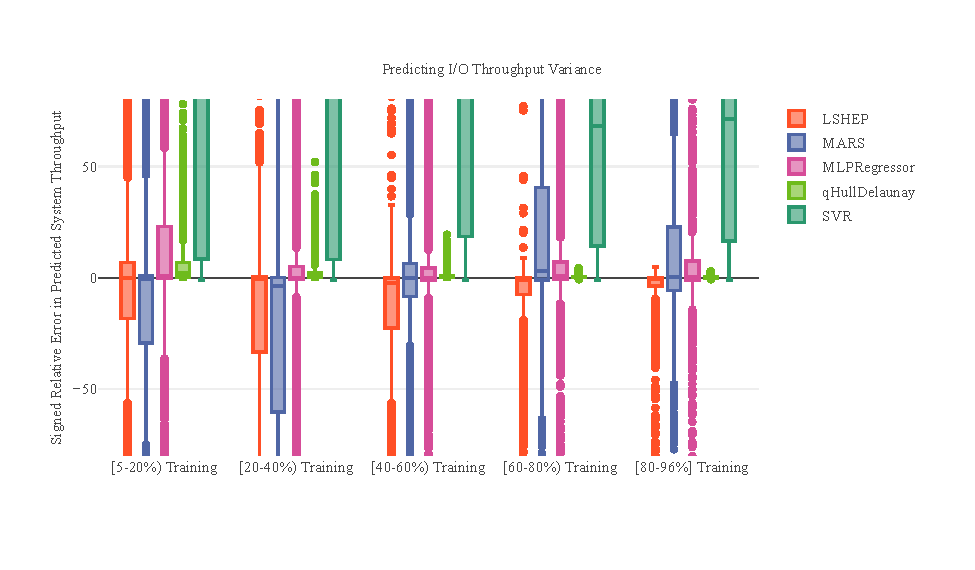
\includegraphics[width=\textwidth,trim={0 .5in 0 .3in}]{Figures/HPC/Var_TT_Ratio.pdf}
  \caption{These box plots show the prediction error of variance with
    increasing amounts of training data provided to the models. The
    response values being predicted span six orders of magnitude. For
    SVR the top box whisker goes from around 6000 to 400 (decreasing
    by factors of 2) from left to right and is truncated in order to
    maintain focus on better models. Results for all dimensions are
    aggregated. Max training percentage is 96\% due to rounding
    training set size.}
  \label{fig:var_tt_ratio}
\end{figure}
 

\subsection{I/O Throughput Variance}

The prediction results for variance resemble those for
predicting mean. Delaunay remains the best overall predictor
(aggregated across training percentages and dimensions) with median
relative error of .47 and LSHEP closely competes with Delaunay having
a median signed relative error of -.92. Outliers in prediction error
are much larger for all models. Delaunay produces relative errors as
large as 78 and other models achieve relative errors around
$10^3$. The relative errors for many models scaled proportional to the
increased orders of magnitude spanned by the variance response
compared with mean response. As can be seen in Figure
\ref{fig:var_tt_ratio}, all models are more sensitive to the amount of
training data provided than their counterparts for predicting mean.

\subsection{Increasing Dimension and Decreasing Training Data}

As can be seen in Figure \ref{fig:mean_dim}, all of the models suffer
increasing error rates in higher dimension. This is expected, because
the number of possible interactions to model grows
exponentially. However, LSHEP and Delaunay maintain the slowest
increase in relative error. The increase in error seen for Delaunay
suggests that it is capable of making predictions with a range of
relative errors that grows approximately linearly with increasing
dimension input. This trend suggests that Delaunay would remain a
viable technique for accurately modeling systems with 10's of
parameters given only small amounts of training data. All models, with
the exception of MARS, produce smaller errors given more training
data. Increasing the amount of training data most notably reduces the
number of prediction error outliers.

%     Discussion     
%====================
\section{Discussion of Na\"{\i}ve Approximations}

The results presented above demonstrate that a straightforward
application of multivariate modeling techniques can be used to
effectively predict HPC system performance. Some modeling effort on
the part of a systems engineer combined with a significant amount of
experimentation (days of CPU time for the IOzone data used here) can
yield a model capable of accurately tuning an HPC system to the
desired performance specification, although qualitatively correct
predictions can be achieved with much less (10\%, say) effort.

\subsection{Modeling the System}

The modeling techniques generated estimates of drastically different
quality when predicting I/O throughput mean and variance. A few
observations: SVR has the largest range of errors for all selections
of dimension and amounts of training data; MARS and LSHEP produce
similar magnitude errors while the former consistently underestimates
and the latter consistently overestimates; Delaunay has considerably
fewer outliers than all other methods. SVR likely produces the poorest
quality predictions because the underlying parametric representation
is global and oversimplified (a single polynomial), making it unable
to capture the complex local behaviors of system I/O. It is still
unclear, however, what causes the behaviors of LSHEP, MARS, and
Delaunay. An exploration of this topic is left to future work.

The Delaunay method appears to be the best predictor in the present
IOzone case study. Particularly a piecewise linear interpolant like
Delaunay appears well-suited for prediction when relatively small
amounts of data are available to mode la function. It is important to
note that the Delaunay computational complexity in the dimension of
the input is worse than other techniques.

Finally, the ability of the models to predict variance was
significantly worse than for the I/O mean. The larger scale in
variance responses alone do not account for the increase in relative
errors witnessed. This suggests that system variability has a greater
underlying functional complexity than the system mean and that latent
factors are reducing prediction performance.

\subsection{Extending the Analysis}

System I/O throughput mean and variance are simple and useful system
characteristics to model. The process presented in this chapter is
equally applicable to predicting other useful performance
characteristics of HPC systems such as: computational throughput,
power consumption, processor idle time, context switches, RAM usage,
or any other ordinal performance metric. For each of these there is
the potential to model system variability as well. This chapter uses
variance as a measure of variability, but the techniques are applied
to more precise measures of variability (the entire distribution
itself) in Chapter \ref{ch:strong}.

\vspace{-10pt}
\section{Takeaway From Na\"{\i}ve Approximation}
\label{sec:conclusion}

Multivariate models of HPC system performance can effectively predict
I/O throughput mean and variance. These multivariate techniques
significantly expand the scope and portability of statistical models
for predicting computer system performance over previous work. In the
IOzone case study presented, the Delaunay method produces the best
overall results making predictions for 821 system configurations with
less than 5\% error when trained on only 43 configurations. Analysis
also suggests that the error in the Delaunay method will remain
acceptable as the number of system parameters being modeled
increases. These multivariate techniques should be applied to HPC
systems with more than four tunable parameters in order to identify
optimal system configurations that may not be discoverable via
previous methods nor by manual performance tuning, which will be
explored in later chapters.


%% Introduce the theory on box splines. Introduce the algorithms that rely on box splines. Show the results of the code that produces box splines.
%% Demonstrate the application of these meshes (and box splines particularly) to approximation problems. Discuss results.
\chapter{Box Splines: Uses, Constructions, and Applications} \label{ch:boxes}
Chapter \ref{ch:naive} demonstrated that the modeling and
approximation techniques described in Chapter \ref{ch:algs} can be
used to model and predict numeric approximations of system
variability. The case study was only for four-dimensional data, and
the key weakness of the best predictor (Delaunay) is scaling with
dimension. This Chapter discusses a modeling approach that may achieve
better scaling with dimension, proposes a quasi-mesh construction, and
analyzes the performance of this proposed technique.


\section{Box Splines}
\label{sec_box_splines}

\begin{figure}
  \centering
  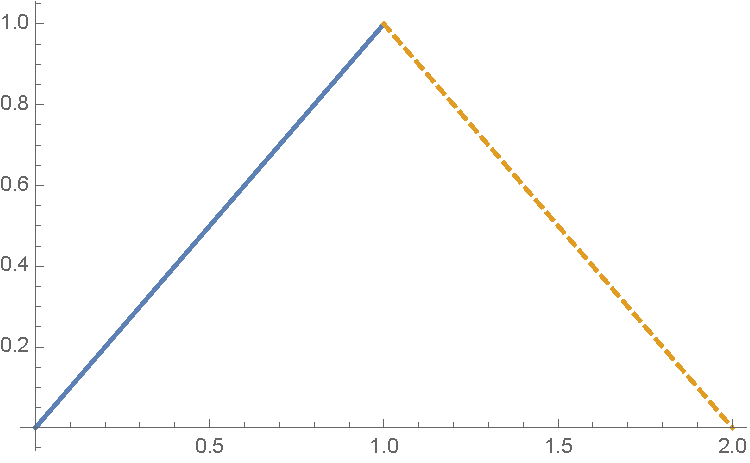
\includegraphics[width=0.45\textwidth]{Figures/ACM/1D-linear.pdf}
  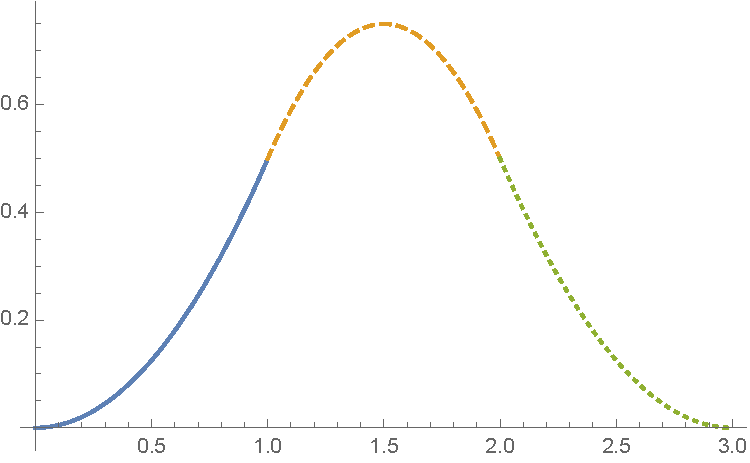
\includegraphics[width=0.45\textwidth]{Figures/ACM/1D-quadratic.pdf}
  \caption{1D linear (order 2) and quadratic (order 3) box splines with direction vector sets $\bigl( 1 \ 1 \bigr)$ and $\bigl( 1 \ 1 \ 1 \bigr)$ respectively. Notice that these direction vector sets form the B-Spline analogues, order 2 composed of two linear components and order 3 composed of 3 quadratic components (colored and styled in plot).}
  \label{fig_1D_boxes}
\end{figure}

\begin{figure}
  \centering
  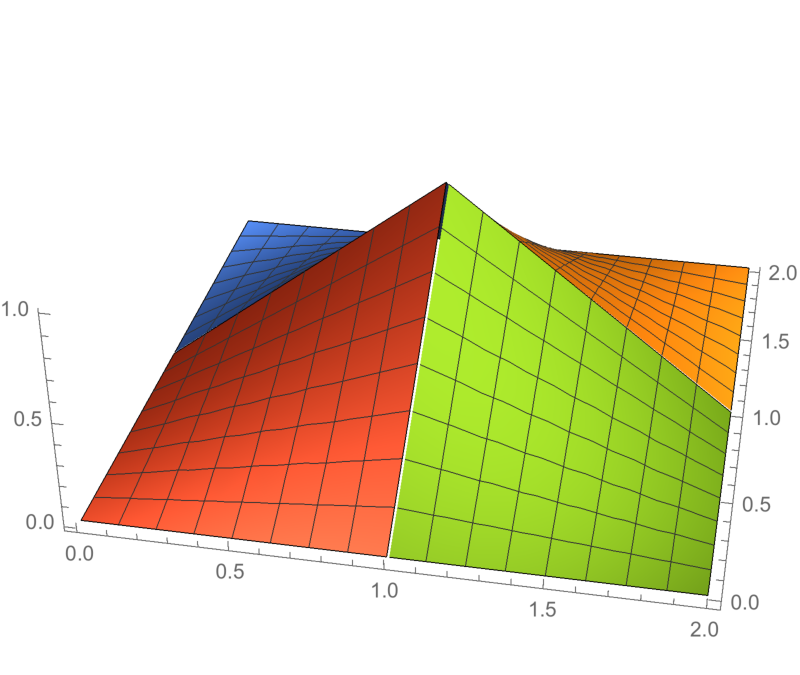
\includegraphics[width=0.45\textwidth]{Figures/ACM/2D-linear.pdf}
  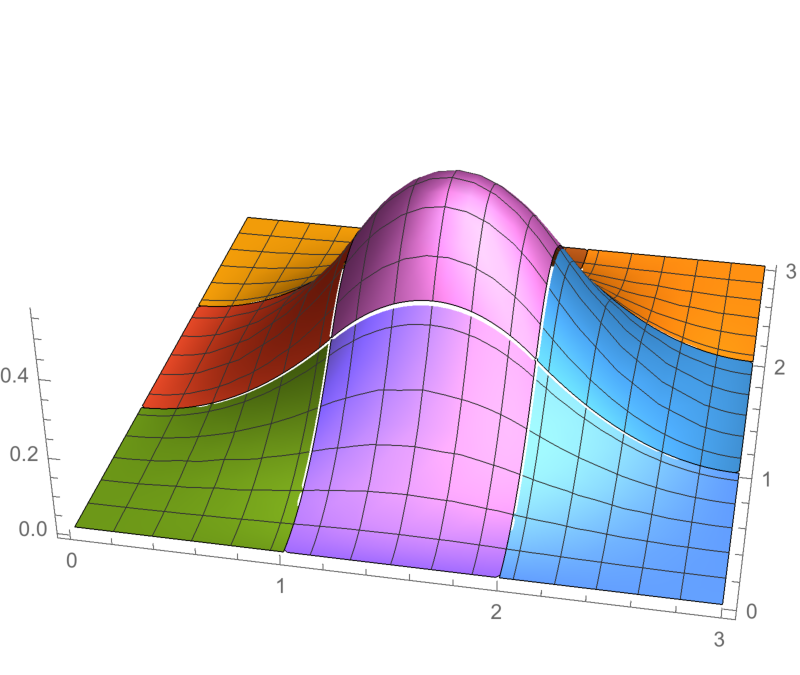
\includegraphics[width=0.45\textwidth]{Figures/ACM/2D-quadratic.pdf}
  \caption{2D linear (order 2) and quadratic (order 3) box splines with direction vector sets $\bigl( I \ I \bigr)$ and $\bigl( I \ I \ I \bigr)$ respectively, where $I$ is the identity matrix in two dimensions. Notice that these direction vector sets also produce boxes with $\text{order}^2$ subregions (colored in plot).}
  \label{fig_2D_boxes}
\end{figure}

A box spline in $\mathbb{R}^d$ is defined by its \textit{direction vector set} $A$, composed of $s$ $d$-vectors where $s \geq d$. Further, $A$ will be written as a $d \times s$ matrix. The first $m$ column vectors of $A$ are denoted by $A_m$, $m \leq s$. $A_d$ is required to be nonsingular. Consider the unit cube in $s$ dimensions $Q_s = [0,1)^s$. $A_s \bigl( Q_s \bigr)$ is now the image (in $d$ dimensions) of $Q_s$ under the linear map $A$. This image is the region of support for the box spline defined by $A_s$ in $d$ dimensions. The box spline function in $d$ dimensions for $A_d$ is defined as
\begin{equation}
B(x \mid A_d) = \begin{cases} 
(\det(A_d))^{-1}, & x \in A_d(Q_d), \\
0,                & \text{otherwise.}
\end{cases}
\label{eq_box_base}
\end{equation}
For $A_s$ when $s > d$ the box spline is computed as
\begin{equation}
B(x \mid A_s) = \int_0^1 B(x - t v_s \mid A_{s-1}) dt,
\label{eq_box_recursive}
\end{equation}
where $v_s$ is the $s$th direction vector of $A$.

The application of box splines presented in this chapter always utilizes the $d$-dimensional identity matrix as $A_d$. This simplifies the computation in Equation \ref{eq_box_base} to be the characteristic function for the unit cube. Composing $A$ strictly out of $k$ repetitions of the identity matrix forms the $k$th order B-spline with knots located at $0$, $1$, $\ldots$, $k-1$, $k$ along each axis (see Figure \ref{fig_1D_boxes}). Furthermore, while the number of subregions for the $k$th order $d$-dimensional box spline grows as $k^d$ (see Figure \ref{fig_2D_boxes}), the symmetry provided by direction vector sets composed of repeated identity matrices allows the computation of box splines to be simplified. The value of a box spline at any location is then the product of all axis-aligned 1-dimensional $k$th order box splines.

The box splines as presented are viable basis functions. Each box spline can be shifted and scaled without modifying the underlying computation (similar to wavelets), yet the underlying computation is simple and scales linearly with dimension. For a more thorough introduction and exploration of box splines in their more general form, readers are referred to \cite{de2013box}. 

\begin{figure}
  \centering
  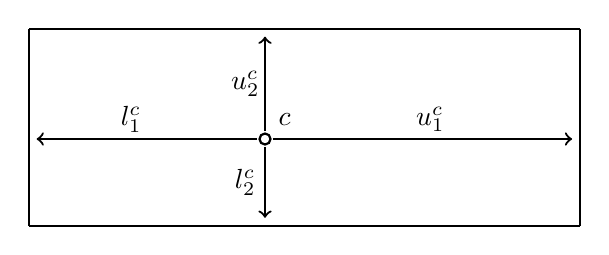
\begin{tikzpicture}[scale=1]
    \draw[thick] (3,1.1) circle (0.7mm);

    %% Draw arrows for each width
    \draw[thick,->] (3,1.2) -- (3,2.4);
    \draw[thick,->] (3,1.0) -- (3,0.1);
    \draw[thick,->] (3.1,1.1) -- (6.9,1.1);
    \draw[thick,->] (2.9,1.1) -- (0.1,1.1);

    %% Draw boundary of box
    \draw[thick,-] (0,0) -- (7,0);
    \draw[thick,-] (7,0) -- (7,2.5);
    \draw[thick,-] (7,2.5) -- (0,2.5);
    \draw[thick,-] (0,2.5) -- (0,0);

    %% Add text to the picture
    \node at (3.25,1.35) {$c$};
    \node at (1.3,1.35) {$l^c_1$};
    \node at (5.1,1.35) {$u^c_1$};
    \node at (2.75,0.55) {$l^c_2$};
    \node at (2.75,1.8) {$u^c_2$};
  \end{tikzpicture}
  \caption{An example box in two dimensions with anchor $c$, upper widths $u^c_1$, $u^c_2$, and lower widths $l^c_1$, $l^c_2$. Notice that $c$ is not required to be equidistant from opposing sides of the box, that is $u^c_i \not= l^c_i$ is allowed.}
  \label{fig_example_box}
\end{figure}

Throughout this section, the notation will be reused from Chapter \ref{ch:algs}. $X \subset \mathbb{R}^d$ is a finite set of points with known response values $f(x)$ for all $x \in X$. Also let $L,U \in \mathbb{R}^d$ define a bounding box for $X$ such that $L < x < U$ for all $x \in X$.

Define a box $b^c = (c,l^c,u^c)$ in $d$ dimensions with anchor $c \in \mathbb{R}^d$, lower width vector $l^c \in \mathbb{R}^d_+$, and upper width vector $u^c \in \mathbb{R}^d_+$ (where $u^c_i$ refers to the $i$th component of $u^c$). A visual example of a box in two dimensions can be seen in Figure \ref{fig_example_box}. Now, define a componentwise rescaling function $g: \mathbb{R}^d \rightarrow \mathbb{R}^d$ at point $x \in \mathbb{R}^d$ to be
\begin{equation}
  \bigl(g^c(x)\bigr)_r = {k \over 2} \left( 1 - {(x_r - c_r)_- \over l^c_r} + {(x_r - c_r)_+ \over u^c_r} \right),
\end{equation}
where $y_+=\max\{y,0\}$, $y_-=(-y)_+$, $k$ is the order of the box spline as described in Section \ref{sec_box_splines}. Finally, each box spline in a box mesh can be evaluated as $B^c(x) = B(g^c(x) \mid A)$ presuming the order of approximation implies $A$. Both box meshes described in the following sections use box spline basis functions of this form.

A notable property of boxes defined with the linear rescaling function $g^c$, is that $C^0$ and $C^1$ continuity of the underlying box spline are maintained. $C^0$ continuity is maintained through scaling. $C^1$ continuity is maintained for all box splines with $C^1$ continuity (order $\geq 3$) because the scaling discontinuity is located at $c$, where all box splines (of the presented form) have first derivative zero. All continuity beyond the first derivative is lost through the rescaling function $g^c$.

\section{Max Box Mesh}

The first of the three meshes produces a set of boxes around chosen control points and each box has maximal distance between the control point and the nearest side of the box. This centrality property is one mechanism for creating the largest reasonable regions of support for the underlying basis functions. The individual boxes are constructed via the following procedure given a set of control points $C \subseteq X$, $c^{(i)} \in C$,
\begin{enumerate}
  \item Initialize a box $b^{c^{(1)}} = \bigl(c^{(1)}, (c^{(1)} - L), (U - c^{(1)})\bigr)$. \label{step_init}
  \item Identify $c^{(i)}$ over $\bigl\{ j \bigm| j \ne 1$, $B^{c^{(1)}}\bigl( c^{(j)} \bigr) \ne 0 \bigr\}$ that minimizes $\bigl\|c^{(j)}-c^{(1)}\bigr\|_\infty$.  \label{step_closest}
  \item Change the the box $b^{c^{(1)}}$ along the first dimension $r$ such that $\bigl|\bigl|c^{(1)} - c^{(i)}\bigr|\bigr|_\infty = \bigl\vert c^{(1)} - c^{(i)}\bigr\vert_r $, to exclude $c^{(i)}$ from the support of $B^{c^{(1)}}$. \label{step_shrink}
  \item Repeat steps \ref{step_closest} and \ref{step_shrink} until no point in $C$ is in the support of $B^{c^{(1)}}$ (at most $2d$ times, once for each boundary of a box).
\end{enumerate}

The same process is used to construct boxes around all control points in $C$. In order to improve the generality of the approximation, a set of control points is initially chosen to be well-spaced using a statistical method from \citet{amos2014algorithm}:

\begin{enumerate}
\item Generate a sequence of all pairs of points sorted by ascending pairwise Euclidean distance between points $\bigl(x^{(i_1)},x^{(j_1)}\bigr)$, $\bigl(x^{(i_2)},x^{(j_2)}\bigr)$, $\ldots$ , so that $\bigl\|x^{(i_k)}-x^{(j_k)}\bigr\|_2 \leq \bigl\|x^{(i_{k+1})}-x^{(j_{k+1})}\bigr\|_2$.
\item Sequentially remove points from candidacy until only $|C|$ remain by randomly selecting a single point from each pair $\bigl(x^{(i_m)}, x^{(j_m)}\bigr)$ for $m = 1,\ldots$ if both $x^{(i_m)}$ and $x^{(j_m)}$ are still candidates for removal.
\end{enumerate}

Once the boxes for a max box mesh have been constructed, the parameters can be identified via a least squares fit. The max box mesh (denoted $MBM$) is used to generate a $|X| \times |C|$ matrix $M$ of box spline basis function evaluations at all points in $X$. The solution to the least squares problem $\min_P \bigl\| M \ P - f(X) \bigr\|_2$ is the parameterization of $MBM$. When $C = X$, $M$ is the $|X| \times |X|$ identity matrix, making the max box mesh approximation $\hat f$ an interpolant.

While setting the number of boxes equal to the number of points causes the max box mesh to be an interpolant, the generality of the max box mesh approximation can often be improved by bootstrapping the selection of control points. Given a user-selected batch size $s \leq |X|$, start with $s$ well-spaced control points. Next, measure the approximation error at $x \notin C$ and if the error is too large (determined by user), pick $s$ points at which the magnitude of approximation error is largest, add those points to $C$, and recompute the max box mesh. The user is left to decide the batch size $s$ and the error tolerance based on validation performance and computability. This work uses a batch size of one.

\begin{definition}
The hyperplane $x_r = c_r + u^c_r$ is the upper boundary of box $b^c$ along dimension $r$, and similarly $x_r = c_r - l^c_r$ is the lower boundary of box $b^c$. When the anchor point $y$, for some box $b^y$, lies in the hyperplane (and facet of box $b^c$) defining either boundary along dimension $r$ of $b^c$ it is said that $b^y$ \textit{bounds} $b^c$ in dimension $r$ and is denoted $\bigl( b^c \bigm\vert_r b^y \bigr)$.
\end{definition}

Throughout all experiments and all repeated trials conducted for this study, all tested interpolation points were covered by at least one box in the $MBM$. However, it is possible for the $MBM$ to not form a covering of $[L,U]$ when there are cyclic boundaries. Consider the following example in three dimensions:
\begin{align*}
  C         &= \bigl\{(0,0,0), (1,0,2/3), (1,1,4/3)\bigr\}, \\
  b^{c^{(1)}} &= \bigl( (0,0,0),  \ (*,*,*),  \ (1,*,4/3) \bigr), \\
  b^{c^{(2)}} &= \bigl( (1,0,2/3),\ (1,*,*),  \ (*,1,*)   \bigr), \\
  b^{c^{(3)}} &= \bigl( (1,1,4/3),\ (*,1,4/3),\ (*,*,*)   \bigr).
\end{align*}
Asterisks are used to represent boxes that are not bounded by other boxes along some dimensions. The point $(2,2,-3)$ is not in any of the max boxes defined above. In this case, there is a cycle in box boundaries that looks like $\bigl( b^{c^{(1)}} \bigm\vert_1 b^{c^{(2)}} \bigm\vert_2 b^{c^{(3)}} \bigm\vert_3 b^{c^{(1)}} \bigr)$. This example demonstrates that it is geometrically possible for the max box mesh to fail to cover a space, however experiments demonstrate that it is empirically unlikely.

The max box mesh remains a viable strategy for computed approximations. Given a maximum of $c$ control points in $d$ dimensions with $n$ points, the computational complexities are: $\mathcal{O}(c^2 d)$ for computing boxes, $\mathcal{O}(c d^2 + d^3)$ for a least squares fit, and $\mathcal{O}(n / s)$ for bootstrapping (which is multiplicative over the fitting complexities). Evaluating the max box mesh requires $\mathcal{O}(c d)$ computations.

\section{Iterative Box Mesh}

The iterative box mesh ($IBM$) comprises box-shaped regions that each contain exactly one control point in their interior just as in the $MBM$. However, the mesh is a covering for $[L,U]$ by construction and places boxes in a way that reduces apparent error. The boxes are constructed via the following procedure given a finite set of points $X \subset \mathbb{R}^d$, where $C \subseteq X$ is the (initially empty) set of control points.
\begin{enumerate}
\item Add the box that covers $[L,U]$ anchored at the most central point $x^{(k)} \in X$, add $x^{(k)}$ to $C$, and least squares fit the $IBM$ model to all $x \in X$.
\item Add a new box $[L,U]$ anchored at $x^{(i)} \notin C$ such that $\bigl| IBM(x^{(i)}) - f(x^{(i)}) \bigr| = \max_{x \in X \backslash C} \bigl| IBM(x) - f(x) \bigr|$, reshaping all boxes $b^{x^{(j)}}$ that contain $x^{(i)}$ by bounding the first dimension $r$ such that $\bigl| x^{(j)}_r - x^{(i)}_r \bigr| = \bigl\| x^{(j)} - x^{(i)} \bigr\|_\infty$ (also reshaping the box $b^{x^{(i)}}$ symmetrically), add $x^{(i)}$ to $C$, and then least squares fit the $IBM$ model to all $x \in X$. \label{step_add_box}
\item Repeat Step \ref{step_add_box} until model approximation error is below tolerance $t$.
\end{enumerate}

Just as for the $MBM$, the parameters can be identified via a least squares fit. The iterative box mesh is used to generate a $|X| \times |C|$ matrix $M$ of box spline function evaluations at all points in $X$. Now the box spline coefficients are the solution to the least squares problem $\min_P \bigl|\bigl| M\ P - f(X) \bigr|\bigr|_2$. Also as for the $MBM$, $C = X$ causes $M$ to equal the $|X| \times |X|$ identity, making the iterative box mesh approximation $\hat f$ an interpolant.

As opposed to the max box mesh, the bootstrapping procedure is built into the iterative box mesh. The user is left to decide the most appropriate error tolerance, however a decision mechanism and analysis is presented in Section \ref{sec_performance_analysis}. As mentioned earlier, the iterative box mesh is a covering for $[L,U]$ by construction and this can be proved by an inductive argument.

An $IBM$ least squares fit $\hat f(z) = \sum_{j}P_j B^{c^{(i_j)}}(z)$ can generate approximations at new points $z \in Z \subset \mathbb{R}^d$ by evaluating $\hat f(z)$. The computational complexity for generating the mesh is $\mathcal{O}(c^2 n d)$ where $c$ is the number of control points determined by the minimum error threshold and $n = |X|$. The computational complexity of evaluating the mesh at a single point is $\mathcal{O}(c d)$.

\section{Voronoi Mesh}


\begin{figure}
  \centering
  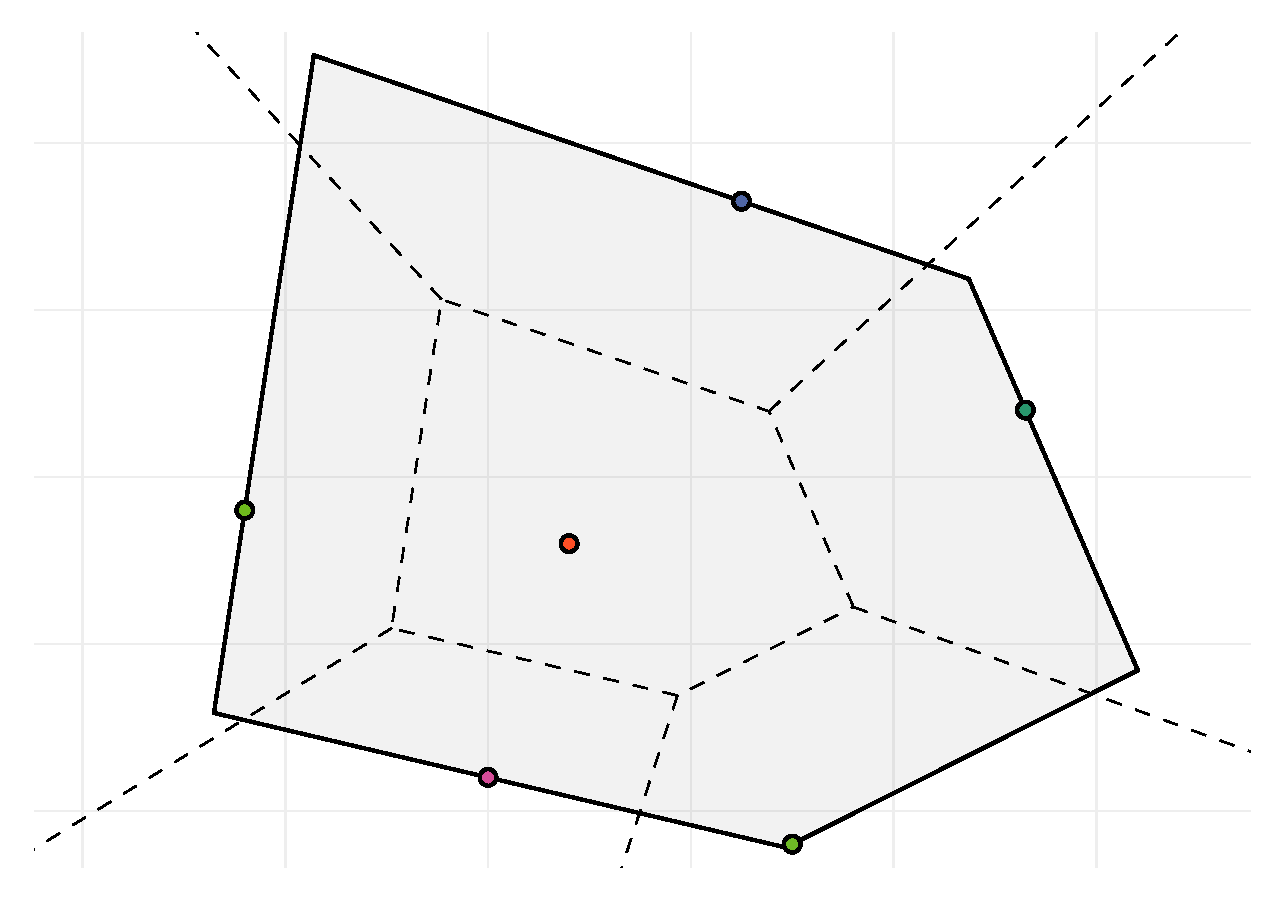
\includegraphics[width=0.6\textwidth,]{Figures/NA/VM_Construction.pdf}
  \caption{Above is a depiction of the Voronoi cell
    boundaries (dashed lines) about a set of interpolation points
    (dots) in two dimensions. In this example, the Voronoi mesh basis
    function about the center most point has nonzero weight in the
    shaded region and transitions from a value of one at the point to
    zero at the boundary of the twice expanded Voronoi cell (solid
    line).
  \vspace{-.1cm}}
  \label{fig:voronoi-basis}
\end{figure}

The final of the three meshes utilizes 2-norm distances to define boundaries rather than max norm distances. It also does not rely on box splines as the underlying basis function. A well-studied technique for classification and approximation is the nearest neighbor algorithm \cite{cover1967nearest}. Nearest neighbor inherently utilizes the convex region $v^{x^{(i)}}$ (Voronoi cell \cite{dirichlet1850reduction}) consisting of all points closer to $x^{(i)}$ than any other point $x^{(j)}$. The Voronoi mesh smooths the nearest neighbor approximation by utilizing the Voronoi cells to define support via a generic basis function $V: \mathbb{R}^d \rightarrow \mathbb{R}_+$ given by

$$ V^{x^{(i)}}(y) = \left(1 - \frac{\bigl\|y - x^{(i)}\bigr\|_2}{2 \ d(y \mid x^{(i)})} \right)_+, $$
where $x^{(i)}$ is the center of the Voronoi cell, $y \in \mathbb{R}^d$ is an interpolation point, and $d(y \mid x^{(i)})$ is the distance between $x^{(i)}$ and the boundary of the Voronoi cell $v^{x^{(i)}}$ in the direction $y - x^{(i)}$. $V^{x^{(i)}}\bigl(x^{(j)}\bigr) = \delta_{ij}$ and $V^{x^{(i)}}$ has local support. While $V^{x^{(i)}}(x^{(i)}) = 1$, the $2$ in the denominator causes all basis functions to go linearly to $0$ at the boundary of the twice-expanded Voronoi cell. Note that this basis function is $C^0$ because the boundaries of the Voronoi cell are $C^0$. In the case that there is no boundary along the vector $w$, the basis function value is always $1$.

While the cost of computing the exact Voronoi cells for any given set of points grows exponentially \cite{dutour2009complexity}, the calculation of $d$ is linear with respect to the number of control points and dimensions. Given any center $x^{(i)} \in \mathbb{R}^d$, set of control points $C \subseteq X$, and interpolation point $y \in \mathbb{R}^d$, $d\bigl(y \mid x^{(i)}\bigr)$ is the solution to
\begin{equation}
  \max_{c \in C\backslash\{x^{(i)}\}} \frac{\bigl\|y - x^{(i)}\bigr\|_2}{2} \ \frac{y \cdot \bigl(c - x^{(i)}\bigr) - x^{(i)} \cdot \bigl(c - x^{(i)}\bigr)}{c \cdot \bigl(c - x^{(i)}\bigr) - x^{(i)} \cdot \bigl(c - x^{(i)}\bigr)}.
\end{equation}

The parameters of the $VM$ can now be computed exactly as for the $MBM$ and $IBM$. The Voronoi mesh is used to generate a $|X| \times |C|$ matrix $M$ of basis function evaluations at all points in $X$. Now the $VM$ coefficients are the solution to the least squares problem $\min_P \bigl\| M \ P - f(X) \bigr\|_2$. When $X = C$, $M$ is the identity making the mesh an interpolant. Bootstrapping can be performed with an identical procedure to that for the $IBM$.
\begin{enumerate}
\item Pick the most central point $x^{(k)} \in X$ to be the first control point in $C$ and fit the $VM$ model to all $x \in X$.
\item Identify a control point $x^{(i)} \notin C$ such that $\bigl| VM(x^{(i)}) - f(x^{(i)}) \bigr| = \max_{x \in X \backslash C} \bigl| VM(x) - f(x) \bigr|$, add $x^{(i)}$ to $C$, and then fit the $VM$ model to all $x \in X$. \label{step_add_control}
\item Repeat Step \ref{step_add_control} until approximation error is below tolerance $t$.
\end{enumerate}

Any $VM$ is na\"{\i}vely a covering for $[L,U]$, since any possible interpolation point will have a nearest neighbor control point. The computational complexity of evaluating a parameterized Voronoi mesh with $c$ control points is $\mathcal{O}(c^2 d)$. Bootstrapping the generation of a Voronoi mesh requires $\mathcal{O}(c^2 n d)$ computations for a maximum number of basis functions $c$ determined by the error threshold.



% Art is a subjective form of personal expression and computers are just robots that are going to take over the world. \textit{*deep breath*} In order to communicate my frustration with the technological and information revolution, I'm going to write the rest of this paper in poetry.

% Star light, star bright \ldots

% \subsection{Boxed Natural Neighbor}
% \begin{itemize}
% \item How the mesh is generated
% \item How interpolation is done
% \end{itemize}

\section{Data and Analysis}

Some data sets will be used to evaluate the interpolation and regression meshes proposed above. This chapter utilizes three data sets of varying dimension and application. In the following subsections the sources and targets of each data set are described, as well as challenges and limitations related to interpolating and approximating these data sets. The distributions of response values being modeled can be seen in Figure \ref{fig_response_hists}. The preprocessing and approximation processes are described in Section \ref{sec_performance_analysis}.

\begin{figure}
  \centering
  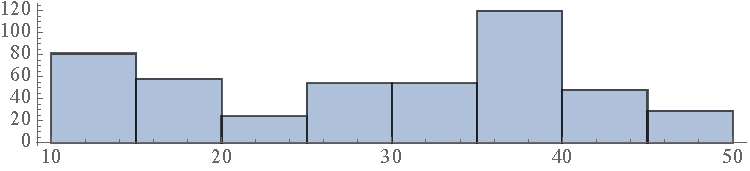
\includegraphics[width=.8\textwidth]{Figures/ACM/p-hist.pdf}
  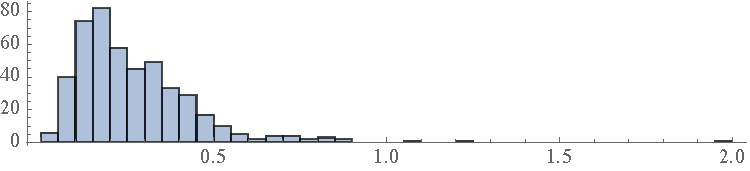
\includegraphics[width=.8\textwidth]{Figures/ACM/f-hist.pdf}
  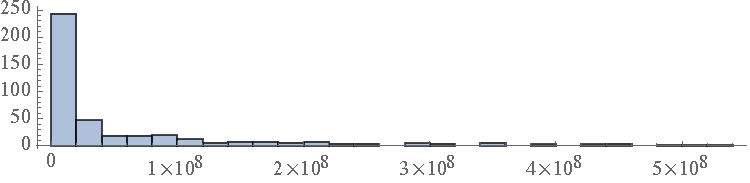
\includegraphics[width=.8\textwidth]{Figures/ACM/h-hist.pdf}
  \caption{Histograms of Parkinsons (total UPDRS), forest fire (area), and HPC I/O (mean throughput) response values respectively. Notice that both the forest fire and HPC I/O data sets are heavily skewed.
  \vspace{-.5cm}}
  \label{fig_response_hists}
\end{figure}

\subsection{High Performance Computing I/O ($n = 532, d = 4$)}
The first of three data sets is a four-dimensional data set produced by executing the IOzone benchmark from \cite{iozone} on a homogeneous cluster of computers. The system performance data was collected by executing IOzone 40 times for each of a select set of system configurations. A single IOzone execution reports the max I/O file-read throughput seen. The 40 executions for each system configuration are converted to their mean, which is capable of being modeled by each of the multivariate approximation techniques presented earlier in this chapter. The four dimensions being modeled to predict throughput mean are file size, record size, thread count, and CPU frequency.

\begin{figure*}[htb]
  \centering
  \begin{tikzpicture}
    \node (img)  {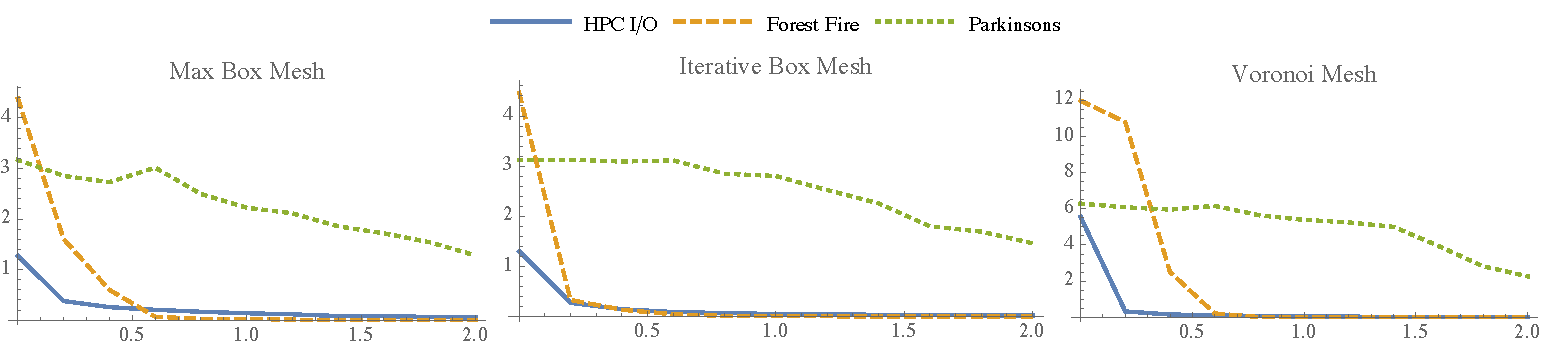
\includegraphics[width=0.95\textwidth,height=4cm]{Figures/ACM/eval-times.pdf}};
    \node[below=of img, node distance=0cm, yshift=1cm] {Relative Error Tolerance while Bootstrapping};
    \node[left=of img, node distance=0cm, rotate=90, anchor=center,yshift=-0.7cm] {Fit Time};
  \end{tikzpicture}
  \caption{Time required to generate model fits for each technique with varying relative error tolerance during bootstrapping.
    \vspace{-.3cm}}
  \label{fig_eval_times}
\end{figure*}

\subsection{Forest Fire ($n = 517, d = 12$)}
The forest fire data set \cite{cortez2007data} describes the area of Montesinho park burned on specific days and months of the year in terms of the environmental conditions. The twelve dimensions being used to model burn area are the $x$ and $y$ spatial coordinates of burns in the park, month and day of year, the FFMC, DMC, DC, and ISI indices (see source for details), the temperature in Celsius, relative humidity, wind speed, and outdoor rain. The original analysis of this data set demonstrated it to be difficult to model, likely due to the skew in response values.

\subsection{Parkinson's Telemonitoring ($n = 468, d = 16$)}
The final data set for evaluation \cite{tsanas2010accurate} is derived from a speech monitoring study with the intent to automatically estimate Parkinson's disease symptom development in Parkinson's patients. The function to be predicted is a time-consuming clinical evaluation measure referred to as the UPDRS score. The total UPDRS score given by a clinical evaluation is estimated through 16 real numbers generated from biomedical voice measures of in-home sound recordings.

\subsection{Performance Analysis}
\label{sec_performance_analysis}

The performance of the approximation techniques varies considerably across the three evaluation data sets. Relative errors for the most na\"{\i}ve approximators such as nearest neighbor can range from zero to $\displaystyle \big(\max_x f(x) - \min_x f(x)\big) / \min_x f(x)$ when modeling a positive function $f(x)$ from data. Each of the approximation techniques presented remain within these bounds and all errors are presented in signed relative form $(\hat f(x) - f(x)) / f(x)$. Before the models are constructed all data values (components $x^{(i)}_r$ of $x^{(i)} \in X$) are shifted and scaled to be in the unit cube $[0,1]^d$, while the response values are taken in their original form. All models are evaluated with $10$ random $80/20$ splits of the data.

\begin{table}
  \centering
  \begin{tabular}{c|c|c|c}
    \hline
    \textbf{Data Set} & \textbf{Technique} & \textbf{Tolerance} & \textbf{Average Error}\\
    \hline
    HPC I/O & MBM & 1.2 & 0.597\\
    Forest Fire & MBM & 1.8 & 3.517\\
    Parkinson's & MBM & 0.6 & 0.114\\
    \hline
    HPC I/O & IBM & 0.4 & 0.419\\
    Forest Fire & IBM & 1.8 & 3.615\\
    Parkinson's & IBM & 1.8 & 0.121\\
    \hline
    HPC I/O & VM & 0.2 & 0.382\\
    Forest Fire & VM & 1.0 & 4.783\\
    Parkinson's & VM & 2.0 & 1.824\\
    \hline
  \end{tabular}
  \caption{The optimal error tolerance bootstrapping parameters for each technique and each data set as well as the average absolute relative errors achieved by that tolerance. Notice that large relative error tolerances occasionally yield even lower evaluation errors, demonstrating the benefits of approximation over interpolation for noisy data sets.
  \vspace{-.5cm}}
  \label{tab_optimal_tolerance}
\end{table}

Each of the approximation techniques presented incorporates bootstrapping based on an allowable error tolerance $t$. An analysis of the effects of bootstrapping error tolerances on validation accuracy can be seen in Figure \ref{fig_all_performance}. The approximation meshes perform best on the forest fire and Parkinson's data sets when the error tolerance used for fitting is large (smoothing rather than interpolating), while near-interpolation generally produces the most accurate models for HPC I/O. Another performance result of note is that the $MBM$ and $IBM$ have very similar basis functions with largely different outputs.

\begin{figure*}
  \begin{tikzpicture}
    \node (img)  {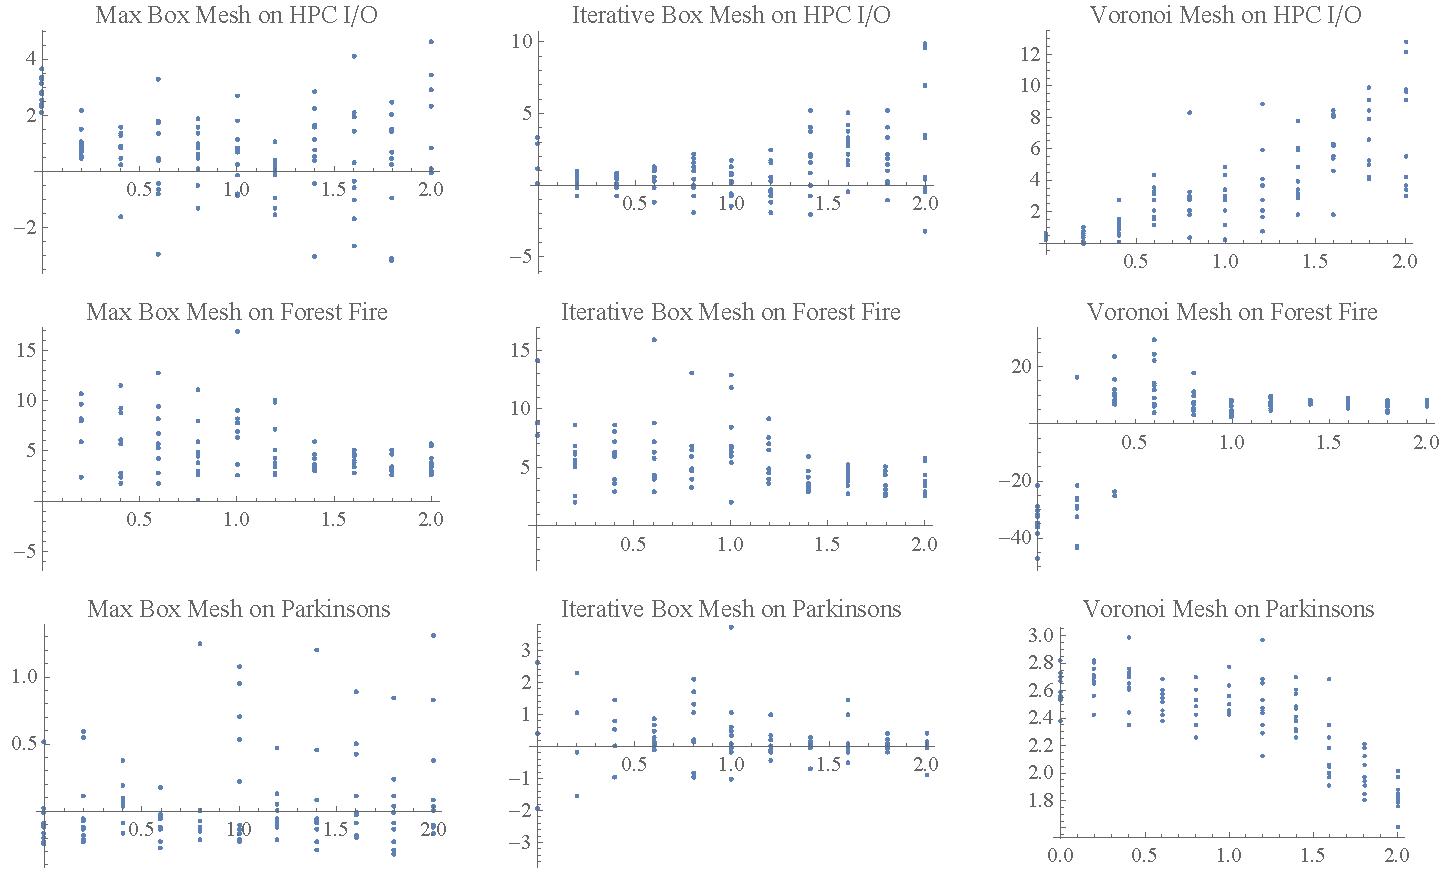
\includegraphics[width=0.95\textwidth,height=9.5cm]{Figures/ACM/all-performance.pdf}};
    \node[below=of img, node distance=0cm, yshift=1cm] {Relative Error Tolerance while Bootstrapping};
    \node[left=of img, node distance=0cm, rotate=90, anchor=center,yshift=-0.7cm] {Signed Relative Error};
  \end{tikzpicture}
  \caption{The performance of all three techniques with varied relative error tolerance for the bootstrapping parameter. The columns are for Max Box Mesh, Iterative Box Mesh, and Voronoi Mesh, respectively. The rows are for HPC I/O, Forest Fire, and Parkinson's respectively. Notice the techniques' behavior on the Parkinson's and Forest Fire data sets, performance increases with larger error tolerance.}
  \label{fig_all_performance}
\end{figure*}

\begin{figure*}
  \begin{tikzpicture}
    \node (img)  {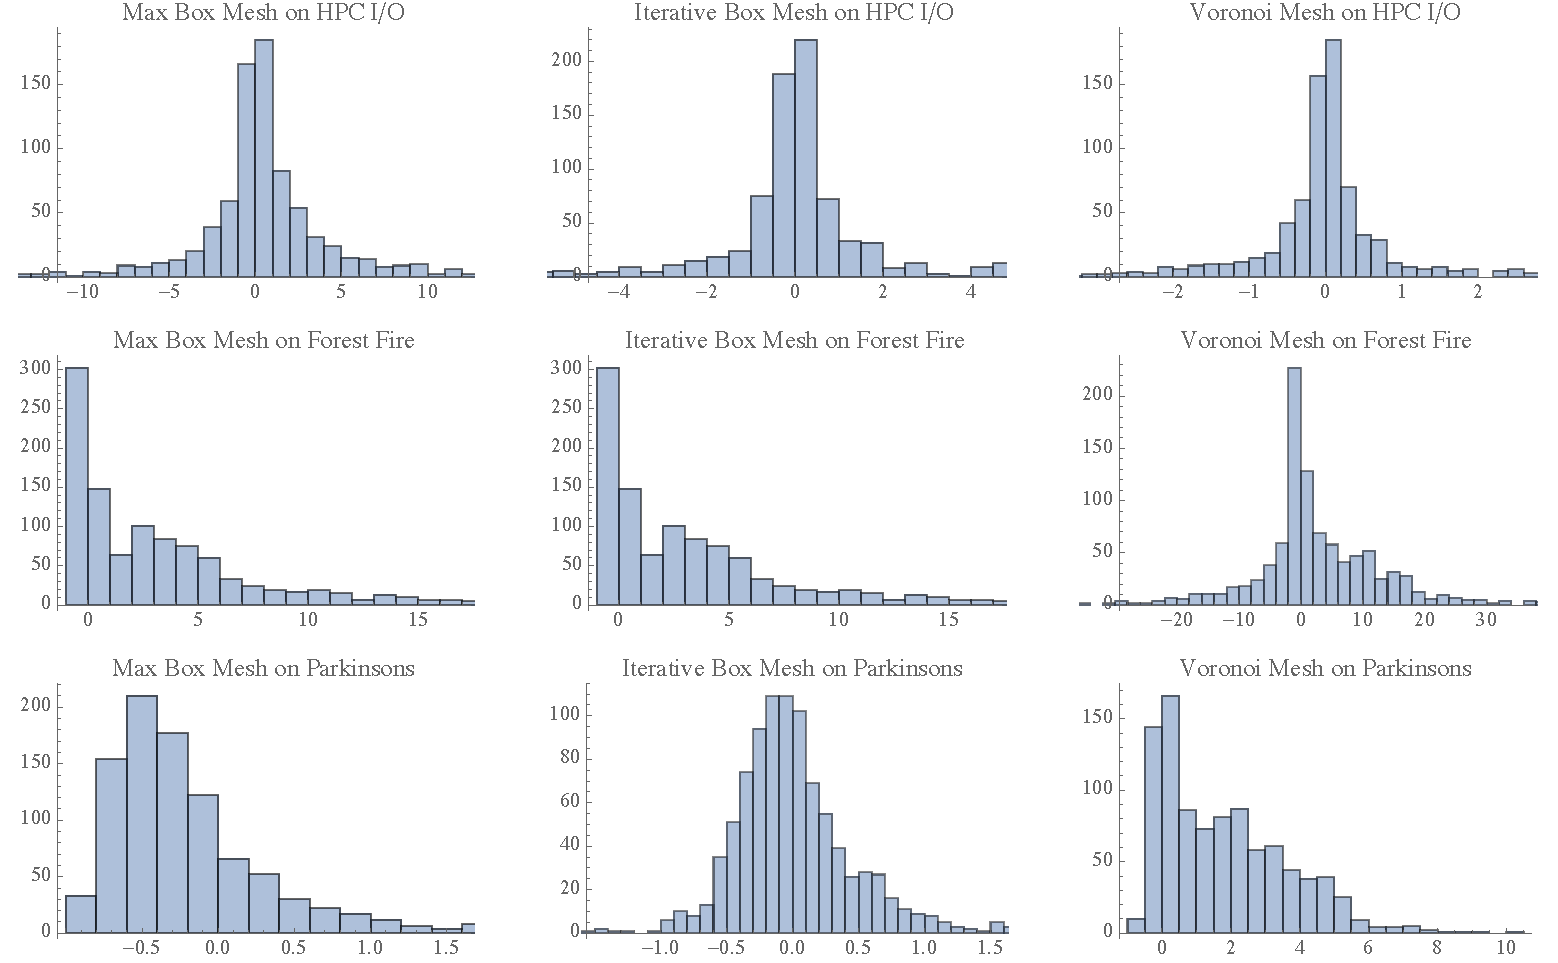
\includegraphics[width=0.95\textwidth,height=9.5cm]{Figures/ACM/perf-sample.pdf}};
    \node[below=of img, node distance=0cm, yshift=1cm] {Signed Relative Error in Prediction};
    \node[left=of img, node distance=0cm, rotate=90, anchor=center,yshift=-0.7cm] {Count};
  \end{tikzpicture}
  \caption{A sample of relative errors for all three techniques with optimal selections of error tolerance. The columns are for Max Box Mesh, Iterative Box Mesh, and Voronoi Mesh, respectively. The rows are for HPC I/O, Forest Fire, and Parkinson's respectively.
    \vspace{-.3cm}}
  \label{fig_perf_sample}
\end{figure*}

The selection of bootstrapping error tolerance also effects the computation time required to fit each of the models to data. Figure \ref{fig_eval_times} presents the time required to construct approximations for each model and each data set with varying $t$. The rapid reduction in computation time required for the forest fire and HPC I/O data sets suggests that large reductions in error can be achieved with relatively few basis functions. The Parkinson's data set however presents a more noisy response, with increasing number of basis functions reducing error much less quickly.

The distributions of errors experienced by each approximation technique when the optimal bootstrapping relative error tolerance is selected can be seen in Figure \ref{fig_perf_sample}. HPC I/O exhibits the most normal approximation errors, which suggests that the models are converging on the random noise of the response for the data set. The worst relative approximation errors are produced by the Voronoi mesh on the forest fire data set. The small magnitude true response values contribute to the larger relative errors. Regardless, the $VM$ errors are unacceptably large.

\section{Discussion of Mesh Approximations}

The bootstrapping procedure presented for each quasi-mesh approximation is very computationally expensive and does not provide much improvement over the interpolatory approach. Analysis suggests that the appropriate relative error tolerance needs to be discovered empirically for each application of a modeling technique. Further analytic studies could arrive at methods for determining optimal error tolerances at runtime, however increases in runtime complexity may not be afforded in many applications. 

The box-shaped basis functions and the construction algorithms used for the $MBM$ and $IBM$ could become a source of error when $d$ (the dimension of the data $X$) is comparable to $n$ (the number of known points). The blending regions in which multiple basis functions overlap are always axis aligned and in applications such as image analysis, any single dimension may be unsuitable for approximating the true underlying function. The Voronoi mesh attempts to address this problem by utilizing boundaries between points in multiple dimensions simultaneously. However, it is empirically unclear whether the true benefits of the $VM$ are seen in applications where $d \ll n$.

Each of the case studies presented have fewer than $1000$ points. The complexity of the presented approximation techniques are suitable for large dimension, but the increased complexity associated with brute-force bootstrapping prohibits their use on larger data sets. The Voronoi mesh in particular has a large complexity with respect to $n$ which could be significantly improved by dropping bootstrapping, as is done in Chapter \ref{ch:strong}. While each technique requires less than ten seconds on average to produce a fit in the presented case studies, the fit time required quickly grows into minutes around $1000$ points. These results demonstrate the limits of expensive bootstrapping. However, the viability of each mesh encourages the further applications explored in later chapters.

\section{Implications of Quasi-Mesh Results}

The Max Box Mesh, Iterative Box Mesh, and Voronoi Mesh each provide novel strategies for effectively approximating multivariate phenomonon. The underlying constructions are theoretically straightforward. The computational complexities of each make them particularly suitable for applications in many dimensions, while the bootstrapping error tolerance parameter allows a balance between smoothing and interpolation to be explored empirically with each application. However, the expense of bootstrapping prohibits its use on larger data sets.



%% Introduce a measurement for error when predicting distribution outputs, then show what happens when system behavior is predicted as a distribution.
\chapter{Stronger Approximations of Variability} \label{ch:strong}

Performance and its variability can be summarized by a variety of statistics. Mean, range, standard deviation, variance, and interquartile range are a few summary statistics that describe performance and variability. However, the most precise characterization of any performance measure is the cumulative distribution function (CDF), or its derivative the probability density function (PDF). Previous techniques for predicting system performance have strictly modeled real-valued summary statistics because there exists a large base of mathematical techniques capable of approximating functions of the form $f: \mathbb{R}^d \rightarrow \mathbb{R}$. However, there is little systems work approximating functions $f: \mathbb{R}^d \rightarrow \{g \mid g: \mathbb{R} \rightarrow \mathbb{R}\}$.

%% ===================================================================
\section{Measuring Error}
\label{sec:error}

\begin{figure}[htb]
  \centering
  \begin{tikzpicture}
    \node (img)  {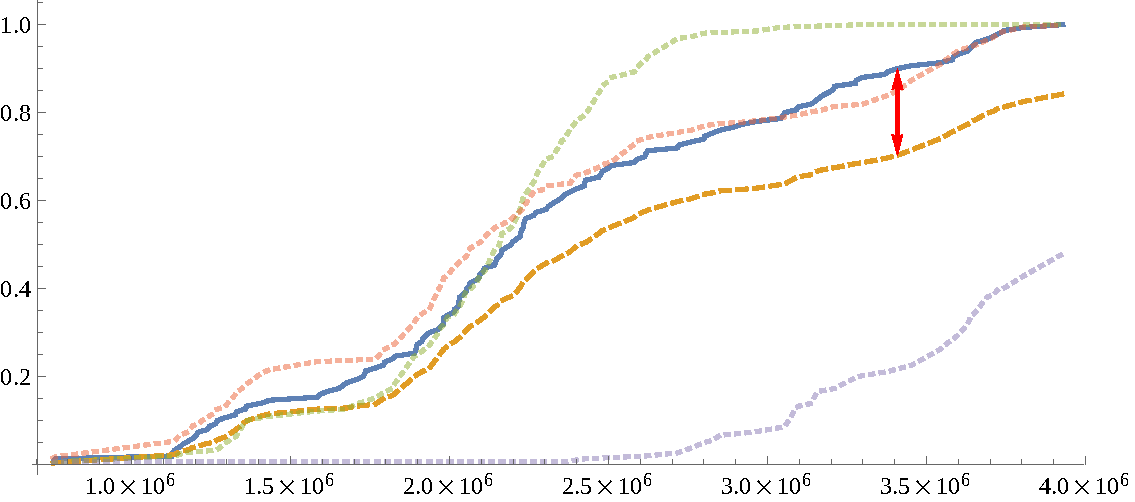
\includegraphics[width=0.75\textwidth,]{Figures/NA/Fig1.pdf}};
    \node[below=of img, node distance=1cm, yshift=1cm] {I/O Throughput};
    \node[left=of img, node distance=0cm, rotate=90, anchor=center,yshift=-0.7cm] {CDF Value};
  \end{tikzpicture}
  \vspace{-0.3cm}
  \caption{In this HPC I/O example, the general methodology for
    predicting a CDF and evaluating error can be seen. The Delaunay
    method chose three source distributions (dotted lines) and
    assigned weights \{.3, .4, .3\} (top to bottom at arrow). The
    weighted sum of the three known CDFs produces the predicted CDF
    (dashed line). The KS Statistic (arrow) computed between the true
    CDF (solid line) and predicted CDF (dashed line) is 0.2 for this
    example. The KS test null hypothesis is rejected at $p$-value
    0.01, however it is not rejected at $p$-value 0.001.}
  \label{fig:prediction-example}
\end{figure}

When the range of an approximation is the real numbers, error is
reported with summary statistics including: min absolute error, max
absolute error, and absolute error quartiles. When the range of an
approximation is the space of cumulative distribution functions, the
Kolmogorov-Smirnov statistic (max-norm difference between the
functions) is used.

A hurdle when modeling function-valued outputs such as cumulative
distribution functions (CDFs) or probability density functions (PDFs)
is that certain properties must be maintained. It is necessary that a
PDF $f: \mathbb{R} \rightarrow \mathbb{R}$ have the properties $f(x)
\geq 0$ and $\int_{-\infty}^{\infty}f(x)dx = 1$. However, for a CDF
$F: \mathbb{R} \rightarrow \mathbb{R}$ the properties are
$F(x) \in [0,1]$ and $F(x)$ is absolutely continuous and
nondecreasing. This work utilizes the fact that a convex combination
of CDFs (or PDFs) results in a valid CDF (or PDF). Given $G(x) =
\sum_{i}w_i F_i(x)$, $\sum_{i} w_i = 1$, $w_i \geq 0$, and each $F_i$
is a valid CDF, $G$ must also be a valid CDF. A demonstration of how
this is applied can be seen in Figure \ref{fig:prediction-example}.

The performance of approximation techniques that predict probability
functions can be analyzed through a variety of summary
statistics. This work uses the max absolute difference, also known as
the Kolmogorov-Smirnov (KS) statistic \cite{lilliefors1967kolmogorov}
for its compatibility with the KS test.

The two-sample KS test is a useful nonparametric test for comparing
two CDFs while only assuming stationarity, finite mean, and finite
variance. The null hypothesis (that two CDFs come from the same
underlying distribution) is rejected at level $p \in [0,1]$ when
 $$ KS > \sqrt{-\frac{1}{2}\ln\biggl(\frac{p}{2}\biggr)} \sqrt{\frac{1}{n_1} + \frac{1}{n_2}}, $$
with distribution sample sizes $n_1,n_2 \in \mathcal{N}$. For all
applications of the KS test presented in this work $n_1 = n_2$. An
example of the round-trip prediction methodology from known and
predicted distributions to the calculation of error can be seen in
Figure \ref{fig:prediction-example}.

%% ===================================================================

\subsection{Feature Weighting}
\label{sec:feature_weighting}

It is well-known that an important procedure in any application of predictive methodologies is identifying those features of the data that are most relevant to making accurate predictions \cite{guyon2003introduction}. Selection strategies such as the floating searches studied in \cite{pudil1994floating} or others compared in \cite{ferri1994comparative} can be too expensive for large approximation problems. Rather, this work poses feature selection as a continuous optimization problem. Let $X$ be an $n \times d$ matrix of $n$ known system configurations with $d$ parameters each normalized to be in $[0,1]$. Define an error function that computes the error of a predictive model trained on $X\hbox{ diag }w$, $w \in \mathbb{R}^d$,  by performing ten random splits with 80\% of the rows of $X\hbox{ diag }w$ for training and 20\% for testing. A minimum of this error function could be considered an optimal weighting of the features of $X$. Minimization is performed using a zero order method in the absence of a readily computable gradient.


%% ===================================================================
\section{Variability Data}
\label{sec:data}

\begin{table}
  \centering
  \begin{tabular}{c|c}
    \hline
    \textbf{System Parameter} & \textbf{Values}\\
    \hline
    File Size (KB) & 4, 16, 64, 256, 1024, 4096, 8192, 16384\\
    \hline
    Record Size (KB) & \multilinecell{4, 8, 16, 32, 64, 128, 256, 512,\\ 1024, 2048, 4096, 8192, 16384}\\
    \hline
    Thread Count & 1, 8, 16, 24, 32, 40, 48, 56, 64\\
    \hline
    Frequency (GHz) & 1.2, 1.6, 2, 2.3, 2.8, 3.2, 3.5\\
    \hline
    Test Type & \multilinecell{Readers, Rereaders, Random Readers, \\ Initial Writers, Rewriters, Random Writers}\\
    \hline
  \end{tabular}
  \caption{A description of system parameters considered for IOzone. Record size must be $\leq$ file size during execution.}
  \label{tab:data_description}
\end{table}

\begin{figure}
  \centering
  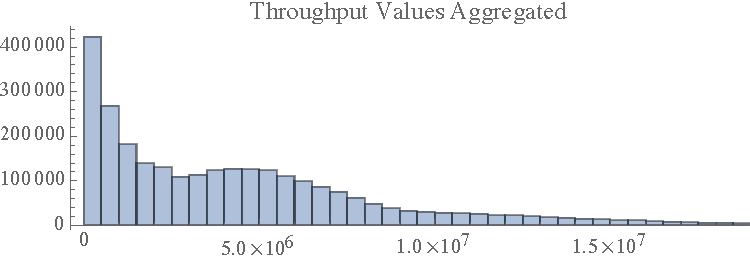
\includegraphics[width=.8\textwidth]{Figures/IEEE/plot-histogram-throughput.pdf}
  \caption{Histogram of the raw throughput values recorded during all IOzone tests across all system configurations. The distribution is skewed right, with few tests having significantly higher throughput than most others.}
  \label{fig:throughput_histogram}
\end{figure}

This chapter utilizes a variability modeling case study with a five-dimensional dataset produced by executing the IOzone benchmark \cite{iozone} on a homogeneous cluster of computers. Each node contains two Intel Xeon E5-2637 CPUs offering a total of 16 CPU cores with 16GB of DRAM. While the CPU frequency varies depending on the test configuration, the I/O from IOzone is performed by an ext4 filesystem sitting above an Intel SSDSC2BA20 SSD drive. At the time of data collection, Linux kernel Version 4.13.0 was used. The system performance data was collected over two weeks by executing IOzone 150 times for each of a select set of approximately 18K system configurations, for a total of approximately 2.7M executions of IOzone. A single IOzone execution reports the max I/O throughput in kilobytes per second seen for the selected test type. The summary of the data components in $x^{(i)}$ for the experiments for this chapter can be seen in Table \ref{tab:data_description}. Distributions of raw throughput values being modeled can be seen in Figure \ref{fig:throughput_histogram}.

Some mild preprocessing was necessary to prepare the data for modeling and analysis. All features were shifted by their minimum value and scaled by their range, mapping each feature independently into $[0,1]$. This normalization ensures each feature is treated equally by the interpolation techniques and should be performed on all data before building models and making predictions regardless of application. All 150 repeated trials for a system configuration were grouped with that configuration. The only nonordinal feature in this data is the test type. All test types were treated as different applications and were separated for modeling and analysis, i.e., predictions for the ``readers'' test type were made using only known configurations for the ``readers'' test type.

%% ===================================================================

\begin{figure}
  \centering
  \begin{tikzpicture}
    \node (img)  {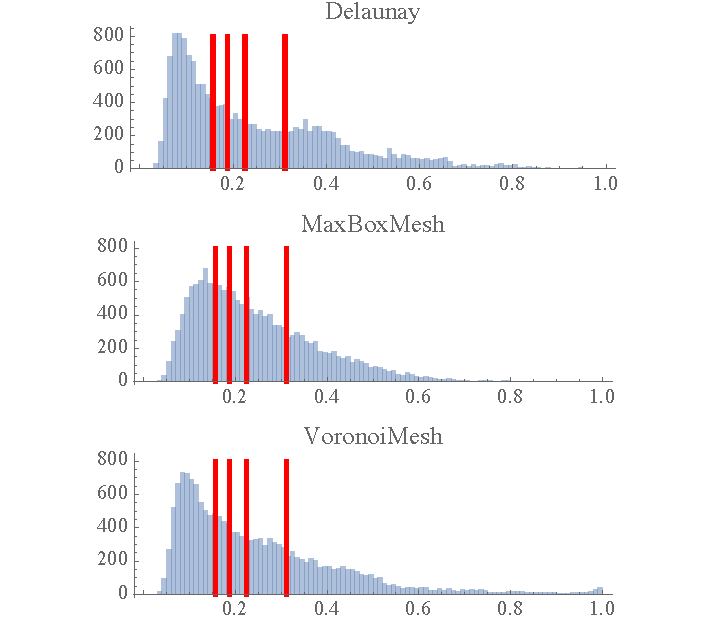
\includegraphics[width=0.8\textwidth,trim={1.5cm 0 0 0}]{Figures/IEEE/plot-histogram-80_20-KS.pdf}};
    \node[below=of img, node distance=1cm, yshift=1cm] {KS Statistic for Predicted vs. Actual};
    \node[left=of img, node distance=0cm, rotate=90, anchor=center,yshift=-0.7cm] {Count of Predictions with Given KS Statistic};
  \end{tikzpicture}
  \caption{Histograms of the prediction error for each modeling algorithm from ten random splits when trained with 80\% of the data aggregated over all different test types. The distributions show the KS statistics for the predicted throughput distribution versus the actual throughput distribution. The four vertical red lines represent commonly used $p$-values \{0.05, 0.01, 0.001, 1.0e-6\} respectively. All predictions to the right of a red line represent CDF predictions that are significantly different (by respective $p$-value) from the actual distribution according to the KS test.}
  \label{fig:ks_histogram_80_20}
\end{figure}

\section{Distribution Prediction Results}

All three interpolation techniques are used to predict the distribution of I/O throughput values at previously unseen system configurations. In order to improve robustness of the error analysis, ten random selections of 80\% of the IOzone data are used to train each model and the remaining 20\% provide approximation error for each model. The recorded errors are grouped by unique system configuration and then averaged within each group. The samples are identical for each interpolation technique, ensuring consistency in the training and testing sets.

The aggregation of errors across all IOzone tests given 80\% of the data as training can be seen in Figure \ref{fig:ks_histogram_80_20}. Agglomerate errors for each technique resemble a Gamma distribution. The percentages of significant prediction errors with varying $p$-values are on display in Table \ref{tab:p_value_failure_rate}. The primary $p$-value used for analyses in this work is 0.001, chosen because close to 2K predictions are made for each test type. Also, applications executed in cloud and HPC systems that could benefit from statistical modeling will be executed at least thousands of times. In line with this knowledge, it is important to ensure that only a small fraction of interpretable results could occur solely under the influence of random chance. When considering the $p=0.001$ results for each technique, a little under half of the predicted CDFs are significantly different from the measured (and presumed) correct CDFs. A rejection rate of 45\% would seem a poor result, however in this situation the complexity of the problem warrants a slightly different interpretation. These predictions are a very \textit{precise} characterization of performance variability, in fact the cumulative distribution function of a random variable is the strongest possible characterization of variability that can be predicted. Globally, only a little under half of the predictions fail to capture \textit{all} of the characteristics of performance variability at new system configurations. It is also demonstrated later in this Section that this result can likely be improved.

\begin{table}
  \centering
  \begin{tabular}{c|c|c}
    \hline
    \textbf{Algorithm} & \textbf{$P$-Value} & \textbf{\% N.H. Rejections} \\
    \hline
    \multilinecell{Delaunay\\Max Box Mesh\\Voronoi Mesh} & .05 & \multilinecell{58.4\\69.3\\61.9}\\
    \hline
    \multilinecell{Delaunay\\Max Box Mesh\\Voronoi Mesh} & .01 & \multilinecell{51.1\\58.4\\53.4}\\
    \hline
    \multilinecell{Delaunay\\Max Box Mesh\\Voronoi Mesh} & .001 & \multilinecell{44.1\\46.9\\45.1}\\
    \hline
    \multilinecell{Delaunay\\Max Box Mesh\\Voronoi Mesh} & 1.0e-6 & \multilinecell{31.4\\26.6\\28.7}\\
    \hline
  \end{tabular}
  \caption{Percent of null hypothesis rejections rate by the KS-test when provided different selections of $p$-values. These accompany the percent of null hypothesis rejection results from Figure \ref{fig:ks_histogram_80_20}.}
  \label{tab:p_value_failure_rate}
\end{table}


While interpreting null hypothesis rejection rates for these interpolation techniques, it is important to consider how the rejection rate reduces with increasing amounts of training data. Figure \ref{fig:ks_failure_by_training} displays the change in $p=0.001$ null hypothesis rejection rate with increasing density of training data up to the maximum density allowed by this set. Delaunay interpolation provides the best results with the least training data by about 5\%, but these low density rejection rates are unacceptably high (90\%). Figure \ref{fig:ks_failure_by_training} clearly shows that this data set and/or the system variables used in the models of performance variability is inadequate to capture the full variability map from system parameters to performance CDF. Which or both obtains is not clear. A few well chosen data points can significantly improve the interpolants, and thus a careful study of the rejection instances is warranted, besides enlarging the set of system variables being modeled.

It may be misleading to consider the global performance of each prediction technique across all test types, as some test types are more difficult than others to predict and have more apparent latent variables. In Figure \ref{fig:ks_failure_by_training_and_test}, the relative difficulty of each IOzone test type can be compared. The I/O test types analyzing reads are typically approximated with lower error than those test types analyzing writes. Regardless of test type, in the aggregate results the KS statistics hover consistently around 0.15, demonstrating an impressively low KS statistic for predictions. In order to address the opacity of aggregate analysis, another case study and an application of the methodology from Section \ref{sec:feature_weighting} is presented in Table \ref{tab:optimized_p_value_failure_rate}.

\begin{figure}
  \centering
  \begin{tikzpicture}
    \node (img)  {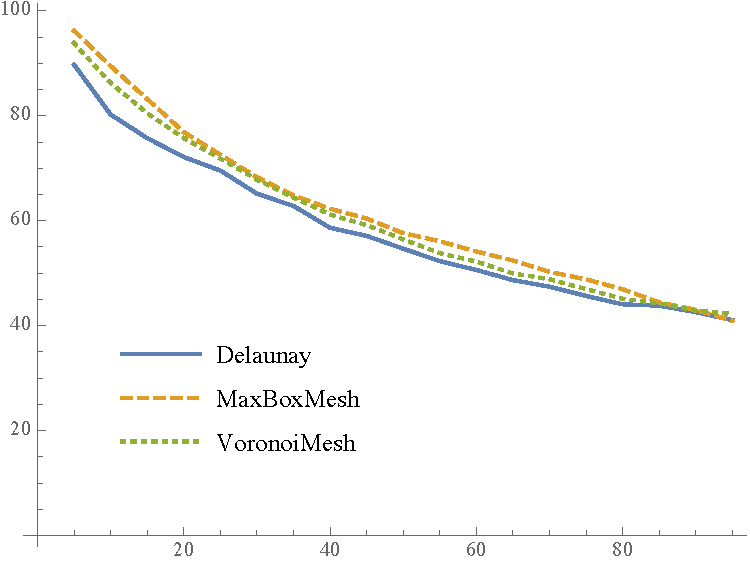
\includegraphics[width=0.8\textwidth,]{Figures/IEEE/plot-KS-Failure-by-Training.pdf}};
    \node[below=of img, node distance=1cm, yshift=1cm] {Percentage of Training Data};
    \node[left=of img, node distance=0cm, rotate=90, anchor=center,yshift=-0.7cm] {\% Null Hypothesis Rejections};
  \end{tikzpicture}
  \caption{The performance of each algorithm on the KS test ($p=0.001$) with increasing amounts of training data averaged over all IOzone test types and ten random splits of the data. The training percentages range from 5\% to 95\% in increments of 5\%. Delaunay is the best performer until 95\% of data is used for training, at which Max Box mesh becomes the best performer by a fraction of a percent.}
  \label{fig:ks_failure_by_training}
\end{figure}

The results presented in Table \ref{tab:optimized_p_value_failure_rate} are achieved by permitting each approximation technique 300 iterations of simulated annealing. In each iteration, the impact of potential weights on the average KS statistic were considered. All weights were kept in the range [0,2], and were applied to the normalized features for frequency, file size, record size, and number of threads. All three approximation techniques had similar optimal weights achieved by simulated annealing of approximately $(.001, 2, 1.7, 1.5)$ for frequency, file size, record size, and number of threads, respectively. Recall that each interpolation technique uses small distances to denote large influences on predictions, meaning that frequency was the most important feature when predicting variability for the ``readers'' test type, followed not-so-closely by number of threads, then record size.

The ``readers'' test type results demonstrate that the underlying prediction techniques work and are capable of seeing rejection rates below 5\% when tuned for a given application. It is important to emphasize that the roughly 95\% of predictions for which the null hypothesis was not rejected are predicting the \textit{precise} distribution of I/O throughput that will be witnessed at a previously unseen system configuration. To the authors' knowledge, there is no existing methodology that is generically applicable to any system performance measure, agnostic of system architecture, and capable of making such powerful predictions.

\begin{table}
  \centering
  \begin{tabular}{c|c|c|c}
    \hline
    \textbf{Algorithm} & \textbf{$P$-Value} & \multilinecell{\textbf{Unweighted}\\\textbf{\% N.H. Rejection}} & \multilinecell{\textbf{Weighted}\\\textbf{\% N.H. Rejection}}\\
    \hline
    \multilinecell{Delaunay\\Max Box Mesh\\Voronoi Mesh} & .05 & \multilinecell{24.9\\21.3\\18.7} & \multilinecell{30.2\\21.2\\11.3}\\
    \hline
    \multilinecell{Delaunay\\Max Box Mesh\\Voronoi Mesh} & .01 & \multilinecell{21.6\\16.4\\14.9} & \multilinecell{27.4\\16.4\\7.0}\\
    \hline
    \multilinecell{Delaunay\\Max Box Mesh\\Voronoi Mesh} & .001 & \multilinecell{19.7\\13.1\\12.3} & \multilinecell{25.4\\13.1\\4.6}\\
    \hline
    \multilinecell{Delaunay\\Max Box Mesh\\Voronoi Mesh} & 1.0e-6 & \multilinecell{17.9\\11.3\\8.5} & \multilinecell{23.4\\11.3\\2.3}\\
    \hline
  \end{tabular}
  \caption{The null hypothesis rejection rates for various $p$-values with the KS-test. These results are strictly for the ``readers'' IOzone test type and show unweighted results as well as the results with weights tuned for minimum error (KS statistic) by 300 iterations of simulated annealing. Notice that the weights identified for the Delaunay model cause data dependent tuning, reducing performance. MaxBoxMesh performance is improved by a negligible amount. VoronoiMesh performance is notably improved.}
  \label{tab:optimized_p_value_failure_rate}
\end{table}

%% \begin{itemize}
%% \item Case studies of good and bad predictions of distributions made, present 3 (best, median, worst)
%% \item Table / Figure showing error for each of the tests (hardest test to predict)
%% \item Presentation of the top most difficult configurations to predict for each test (and the bad performance at those points)
%% %% \item Comparison to predictions made using the "test" numerical column
%% \end{itemize}

\section{Discussion of Distribution Prediction}
\label{sec:discussion}

The results of the IOzone case study indicate that predicting the CDF of I/O throughput at previously unseen system configurations is a challenging problem. The KS statistic captures the worst part of any prediction and hence provides a conservatively large estimate of approximation error. The average absolute errors in the predicted CDFs are always lower than the KS statistics. However, the KS statistic was chosen because of the important statistical theory surrounding it as an error measure. Considering this circumstance, a nonnegligible volume of predictions provide impressively low levels of error. Powerful predictive tools such as those presented in this work allow for more in-depth analysis of system performance variability. For example, system configurations that are most difficult to predict in these tests are likely ``outlier'' configurations that do not resemble those configurations that share many similar parameters. Analysis of these configurations may provide valuable insight into effective application specific operation of computer systems.

As mentioned at the beginning of this chapter, no prior work has attempted to model an arbitrary performance measure for a system to such a high degree of precision. All previous statistical modeling attempts capture a few ($<3$) ordinal performance measures. Generating models that have such high degrees of accuracy allows system engineers to identify previously unused configurations that present desired characteristics. Service level agreements (SLAs) in cloud computing environments are cause for capital competition that is affected heavily by system performance \cite{patel2009service}. Users prefer SLAs that allow the most computing power per monetary unit, incentivizing service providers to guarantee the greatest possible performance. Overscheduling and irregular usage patterns force cloud service providers to occasionally overload machines, in which case precise models of system performance can be used to statistically minimize the probability of SLA violation. Similar targeted performance tuning techniques can be applied to HPC system configuration to maximize application throughput or minimize system power consumption.

A final application domain affected by this methodology is computer security. Collocated users on cloud systems have received attention recently \cite{ali2015security}. If a malicious collocated user is capable of achieving specific insight into the configuration of the system, or the activity of other collocated users by executing performance evaluation programs (i.e., IOzone), a new attack vector may present itself. Malicious users could be capable of identifying common performance distributions of vulnerable system configurations and vulnerable active user jobs. This knowledge may allow targeted exploits to be executed. Light inspection of raw IOzone I/O throughputs provides substantial evidence that distinct performance distributions coincide closely with specific system configuration parameters. Conversely, a service provider may defend against such attacks by deliberately obfuscating the performance of the machine. Models such as those presented in this chapter could identify optimal staggering and time-delay whose introduction into the system would prevent malicious users from identifying system configurations and active jobs.


\begin{figure}
  \centering
  \begin{tikzpicture}
    \node (img)  {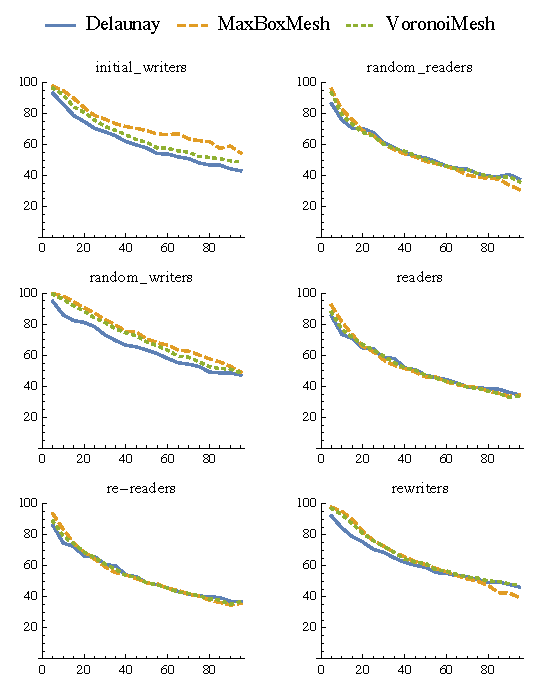
\includegraphics[width=0.8\textwidth,]{Figures/IEEE/plot-KS-failure-by-training-and-test.pdf}};
    \node[below=of img, node distance=1cm, yshift=1cm] {Percentage of Training Data};
    \node[left=of img, node distance=0cm, rotate=90, anchor=center,yshift=-0.7cm] {\% Null Hypothesis Rejections};
  \end{tikzpicture}
  \caption{The percentage of null hypothesis rejections for predictions made by each algorithm on the KS test ($p=0.001$) over different IOzone test types with increasing amounts of training data. Each percentage of null hypothesis rejections is an average over ten random splits of the data. The training percentages range from 5\% to 95\% in increments of 5\%. The read test types tend to allow lower rejection rates than the write test types.}
  \label{fig:ks_failure_by_training_and_test}
\end{figure}


Results presented in Table \ref{tab:optimized_p_value_failure_rate} are particularly interesting, demonstrating that Delaunay appears most vulnerable to data dependent tuning, Max Box mesh is largely insensitive to such tuning, and Voronoi mesh benefits (for this data set) from the tuning.

There are many avenues for extending this modeling methodology. One extension is to add categorical variables to the models. Presently the rejection rate of distribution predictions can only be reduced with large volumes of performance data, however the judicious choice (via experimental design, e.g.) of new data points may be able to effectively reduce the amount of training data required. Finally, more case studies need to be done to test the robustness of the present modeling techniques to changes in domain and performance measure.

\section{The Power of Distribution Prediction}

The methodology presented is capable of providing new insights, extending existing analyses, and improving the management of computational performance variability. Delaunay, Max Box mesh, and Voronoi mesh interpolation are viable techniques for constructing approximations of performance cumulative distribution functions. A case study on I/O throughput demonstrated that the models are capable of effectively predicting CDFs for most unseen system configurations for any of the available I/O test types. The present methodology represents a notable increase in the ability to statistically model arbitrary system performance measures involving the interaction of many ordinal system parameters.


%% Construct error theory that works for all observed applications to this point.
\chapter{An Error Bound on Piecewise Linear Interpolation} \label{ch:error}
%% Apply approximation algorithms to a final set of problems. Discuss results.

This chapter presents theoretical results bounding the error of
(piecewise) linear interpolation. The error analysis relies on linear
interpolation for three reasons: (1) second order results can be
obtained utilizing a Lipschitz constant on the gradient of a function,
rather than standard Lipschitz bounds; (2) the results directly apply
to Delaunay interpolation; and (3) multiple other interpolants in this
paper compute predictions as convex combinations of observed function
values, which may allow for straightforward extensions of this error
bound.

\begin{plainlemma}
  \label{lemma:1}
  Let $S \subset \mathbb{R}^d$ be open and convex, $f: S \rightarrow
  \mathbb{R}$, and let $\nabla f(x)$ be $\gamma$-Lipschitz continuous
  in the $2$-norm. Then for all $x,y \in S$
  $$\big|f(y) - f(x) - \langle \nabla f(x), y - x \rangle \big| \leq \frac{\gamma \|y - x\|_2^2}{2}.$$
\end{plainlemma}

\begin{proofdot}
  Consider the function $g(t) = f \big((1-t) x + t y \big)$, $0 \leq t
  \leq 1$, whose derivative $g'(t) = \big\langle \nabla f \big((1-t) x
  + t y \big), y - x \big\rangle$ is the directional derivative of $f$
  in the direction $(y - x).$
  \begin{align*}
    \big|f(y) - f(x) - \langle &\nabla f(x), y - x \rangle \big|
        = \big|g(1) - g(0) - g'(0) \big| \\
       &= \bigg| \int_0^1 g'(t) - g'(0)\ dt \bigg| \leq \int_0^1 \big|g'(t) - g'(0)\big|\ dt \\
       &= \int_0^1 \bigg| \big \langle \nabla f\big((1-t)x + ty\big) - \nabla f(x), y - x \big \rangle \bigg|\ dt \\
       &\leq \int_0^1 \big \| \nabla f\big((1-t)x + ty\big) - \nabla f(x) \big \|_2\ \| y - x \|_2\ dt \\
       &\leq \int_0^1 \big ( \gamma\ \|y-x\|_2 \big) \ \big( \|y-x\|_2 \big) t\ dt = \frac{\gamma \|y - x\|_2^2}{2}.
  \end{align*}
  \qed
\end{proofdot}

\hfill

\begin{plainlemma}
  \label{lemma:2}
  Let $x, y, v_i \in \mathbb{R}^d$, $c_i \in \mathbb{R}$, and
  $|\langle y - x, v_i \rangle| \leq c_i$ for $i = 1$, $\ldots$, $d.$
  If $M = (v_1$, $\ldots$, $v_d)$ is nonsingular, then
  $$\|y - x\|_2^2 \leq \frac{1}{\sigma_d^2} \sum_{i=1}^d c_i^2,$$
  where $\sigma_d$ is the smallest singular value of $M.$
\end{plainlemma}

\begin{proofdot}
  Using the facts that $M$ and $M^t$ have the same singular values,
  and $\|M^tw\|_2 \geq \sigma_d \|w\|_2$, gives
  \begin{align*}
    \|y - x\|_2^2 &\leq \frac{\|M^t (y - x)\|_2^2}{\sigma_d^2} \\
                  &=    \frac{1}{\sigma_d^2} \sum_{i=1}^d \langle y - x, v_i \rangle^2 \\
                  &\leq \frac{1}{\sigma_d^2} \sum_{i=1}^d c_i^2.
  \end{align*}
  \qed
\end{proofdot}

%% \newpage

\begin{plainlemma}
  \label{lemma:3}
  Given $f$, $\gamma$, $S$ as in {\it Lemma \ref{lemma:1}}, let $X =
  \{x_0$, $x_1$, $\ldots$, $x_d\}$ $\subset S$ be the vertices of a
  $d$-simplex, and let $\hat f(x) = \langle c, x - x_0 \rangle +
  f(x_0)$, $c \in \mathbb{R}^d$ be the linear function interpolating
  $f$ on $X.$ Let $\sigma_d$ be the smallest singular value of the
  matrix $M = (x_1 - x_0$, $\ldots$, $x_d - x_0)$, and $k =
  \max\limits_{1\ \leq\ j\ \leq\ d} \|x_j - x_0\|_2.$ Then
  $$\big\|\nabla f(x_0) - c\big\|_2 \leq \frac{\sqrt{d} \, \gamma k^2}{2 \sigma_d}.$$
\end{plainlemma}

\begin{proofdot}
  \def\g{\gamma_g}
  Consider $g(t)=f(x(t)) - \hat f(x(t))$ along
  the line segment $x(t)=(1-t)x_0 + tx_j$, $0\le t\le1$, from $x_0$ to
  $x_j$.  Observe that $g(0)=f(x_0) - \hat f(x_0) = 0$, $g(1)=f(x_j) -
  \hat f(x_j) = 0$, and $g'(t)$ is $\g$-Lipschitz continuous with $\g
  = \gamma \|x_j-x_0\|_2^2$. The following is visualized in 
  Figure \ref{fig:lemma3}.

  Suppose $g'(0) > \g/2$. Then $|g'(0)-g'(t)| \le \g t \implies g'(0)
  - \g t \le g'(t)$, and the line $w=g'(0)-\g t$ intersects the
  $t$-axis at $\tilde t=g'(0)/\g > 1/2$. $\tilde t<1$ necessarily,
  since by Rolle's Theorem there exists $0<z<1$ such that $g'(z)=0$
  and so $g'(0) - \g z \le g'(z) = 0$. Now by integrating
  $$\frac{g'(0)^2}{2\g} = \frac{g'(0)\tilde t}{2} = \int_0^{\tilde t}
  (g'(0)-\g t)dt \le \int_0^{\tilde t} g'(t)dt = g(\tilde t),$$ and
  using $g'(0) > \g / 2$
  \begin{align*}
    \frac{-g'(0)^2}{2\g} < g'(0) - \frac{g'(0)^2}{2\g} - \g/2 =
    \frac{(1-\tilde t)(g'(0)-\g)}{2} &= \int_{\tilde t}^1 (g'(0)-\g
    t)dt \\ &\le \int_{\tilde t}^1 g'(t)dt = -g(\tilde t),
  \end{align*}
  \noindent a contradiction for the value of $g(\tilde t)$. A similar
  contradiction arises for $g'(0)<-\g/2$. Therefore $|g'(0)| \le
  \g/2$. In terms of $f$,
  $$\bigl|\langle \nabla f(x_0)-c,x_j-x_0\rangle\bigr| = |g'(0)| \le
  \gamma \|x_j-x_0\|_2^2/2 \le \gamma k^2 / 2,$$ which holds for all
  $1\le j\le d$.  Finally, using {\it Lemma \ref{lemma:2}},
  $$\|\nabla f(x_0)-c\|_2^2 \le \frac{d}{\sigma_d^2}(\gamma k^2/2)^2
  \implies \|\nabla f(x_0)-c\|_2 \le \frac{\sqrt{d} \, \gamma
    k^2}{2\sigma_d}.$$ \qed
\end{proofdot}

\begin{figure}
  \centering
  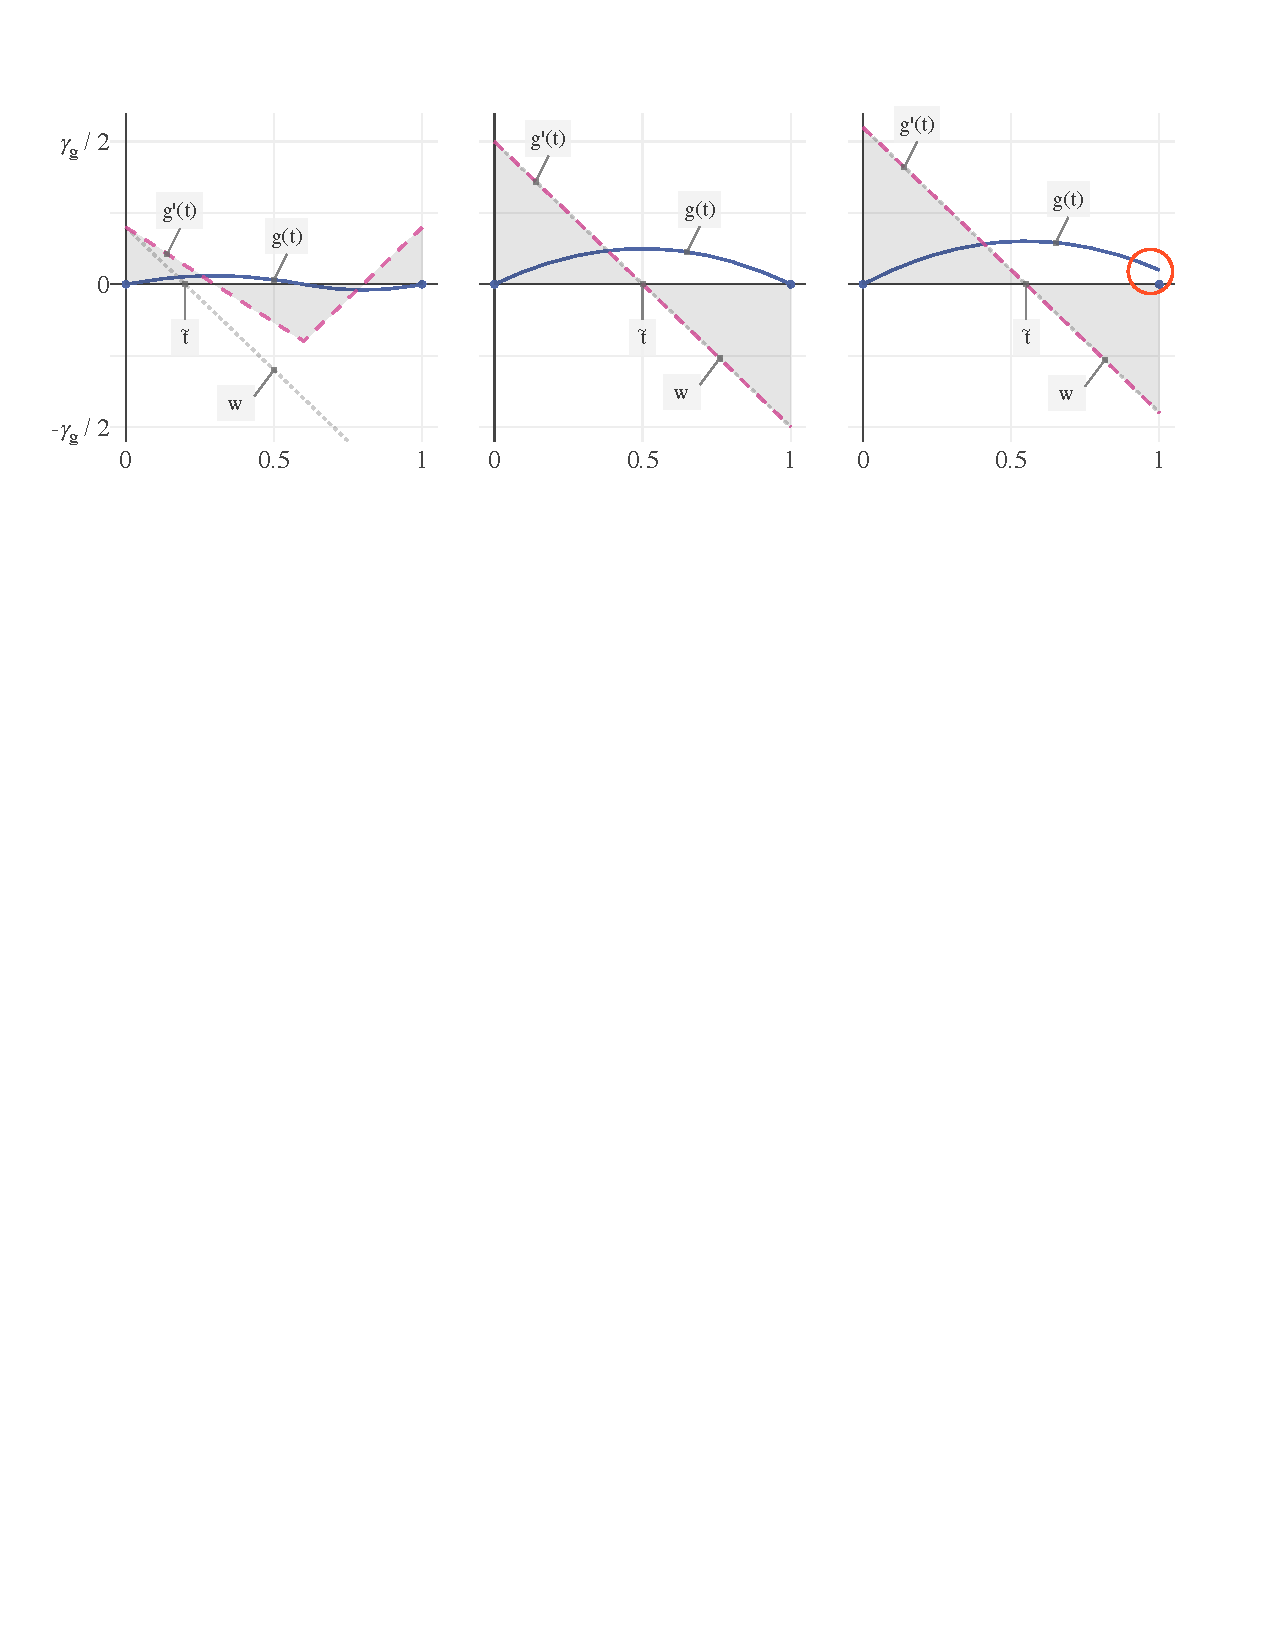
\includegraphics[width=0.9\textwidth,]{Figures/NA/example_lemma_3.pdf}
  \def\g{\gamma_g}
  \caption{Three different scenarios visualizing {\it
      Lemma \ref{lemma:3}}, where $g(t)$ is the difference between a
    piecewise linear interpolant and the approximated function along a
    normalized line segment between interpolation points, $g'(t)$ is
    $\g$-Lipschitz continuous, and $w$ and $\tilde t$ are defined in
    the proof. Leftmost is a randomly chosen permissible shape of $g$
    and $g'$. The middle is the only possible shape of $g$ and $g'$
    given $g'(0) = \g / 2$, establishing the case of equality in the
    lemma. Rightmost is the resulting contradiction when $g'(0) > \g /
    2$, notice it is impossible to ensure $g'(t)$ is $\g$-Lipschitz
    continuous and satisfy $g(1) = 0$ (highlighted with red circle on
    the right).
  \vspace{-.1cm}}
  \label{fig:lemma3}
\end{figure}


\begin{onetheorem}
  Under the assumptions of {\it Lemma \ref{lemma:1}} and {\it Lemma
    \ref{lemma:3}}, for $z \in S$,
  $$ \big|f(z) - \hat f(z)\big| \leq \frac{\gamma \|z - x_0\|_2^2}{2} + \frac{\sqrt{d} \, \gamma k^2}{2 \sigma_d} \|z - x_0\|_2.$$
\end{onetheorem}

\begin{proofdot}
  Let $v = \nabla f(x_0) - c$, where $\|v\|_2 \leq \sqrt{d}\, \gamma k^2 / (2 \sigma_d)$ by {\it Lemma \ref{lemma:3}}. Now
  \begin{align*}
    \big|f(z) - \hat f(z)\big|
       &= \big|f(z) - f(x_0) - \langle c, z - x_0 \rangle \big| \\ 
       &= \big|f(z) - f(x_0) - \langle \nabla f(x_0) - v, z - x_0 \rangle \big| \\
       &= \big|f(z) - f(x_0) - \langle \nabla f(x_0) , z - x_0 \rangle + \langle v , z - x_0 \rangle \big| \\
       &\leq \big|f(z) - f(x_0) - \langle \nabla f(x_0) , z - x_0 \rangle \big| + \big| \langle v , z - x_0 \rangle \big| \\
       &\leq \big|f(z) - f(x_0) - \langle \nabla f(x_0) , z - x_0 \rangle \big| + \|v\|_2 \|z - x_0\|_2 \\
       &\leq \big|f(z) - f(x_0) - \langle \nabla f(x_0), z - x_0 \rangle \big| + \big(\sqrt{d}\,\gamma k^2 / (2 \sigma_d)\big) \|z - x_0\|_2 \\
       &\leq \frac{\gamma \|z - x_0\|_2^2}{2} + \frac{\sqrt{d}\,\gamma k^2}{2 \sigma_d} \|z - x_0\|_2,
  \end{align*}
  where the last inequality follows from {\it Lemma \ref{lemma:1}}.
  %
  \qed
\end{proofdot}


In summary, the approximation error of a linear (simplicial)
interpolant tends quadratically towards zero when approaching observed
data only when the diameter of the simplex is also reduced at a
proportional rate. Only linear convergence to the true function
is achieved in practice without the
incorporation of additional observations, by moving closer to
  interpolation points. Notice that the approximation error is
largely determined by the spacing of observed data. Predictions made
by simplices whose vertices are not well-spaced (i.e., have large
diameter, or are nearly contained in a hyperplane) have higher error.

That the theoretical error bound is sharp can be observed with the
test function $q(x) = \|x\|_2^2,$ $x \in \mathbb{R}^d,$ and the
simplex defined by vertices $X = \{0, e_1, \ldots, e_d\},$ where $e_i$
is the $i$-th standard basis vector in $\mathbb{R}^d,$ $e = (1$,
$\ldots$, $1) \in \mathbb{R}^d,$ and $0$ denotes the zero vector in
any dimension.  The constants relevant to the error bound are
$$ \gamma = 2, \qquad \sigma_d = 1, \qquad k = 1, \qquad x_0 = 0,
\qquad \hat q(x) = \langle e, x - 0\rangle + q(0). $$
\noindent Noting that $q(0) = 0,$ the approximation error at $z =
-(1/2)e$ is
$$ \big|q(z) - \hat q(z)\big| = \big|\|z\|_2^2 - \langle e,z
\rangle\big| = \big| d/4 + d/2 \big| = 3d/4, $$
\noindent while the error bound from the theorem gives

\vspace{-2mm}
\begin{align*}
  \big|q(z) - \hat q(z)\big|
  &\leq \frac{\gamma \|z - x_0\|_2^2}{2} + \frac{\sqrt{d}\,\gamma k}
      {2 \sigma_d} \|z - x_0\|_2 \\
  &{}=  \|z\|_2^2 + \sqrt{d} \|z\|_2 \\
  &{}=  d/4 + d/2 = 3d/4.
\end{align*}
\vspace{-2mm}

\noindent Acknowledging that the error bound is sharp, it may be of
interest to observe the error of piecewise linear approximation
techniques on an analytic test function.

\begin{figure}
  \centering
  \begin{tikzpicture}
    \node (img)  {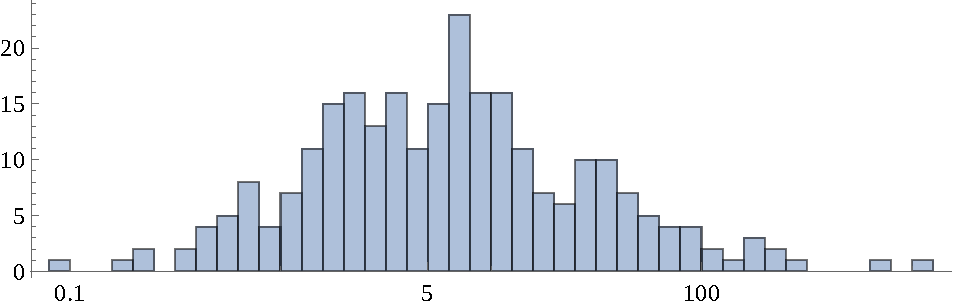
\includegraphics[width=0.9\textwidth,]{Figures/NA/Fig2.pdf}};
    \node[below=of img, node distance=1cm, yshift=1cm] {Number of Data Points};
    \node[left=of img, node distance=0cm, rotate=90, anchor=center,yshift=-0.7cm] {Absolute Error};
  \end{tikzpicture}
  \caption{Delaunay and MLP approximations are constructed from Fekete
    points over the unit cube evaluating the test function $f(x) =
    \cos(\|x\|_2)$ for $x \in \mathbb{R}^2$. The figure shows the
    first/third quartiles at the box bottom/top, the second quartile
    (median) at the white bar, median 95\% confidence interval (cones,
    barely visible in figure), and whiskers at 3/2 of the adjacent
    interquartile ranges, for the absolute prediction error for each
    model at $1000$ random evaluation points. The left plot observes a
    perfect interpolation problem with exact evaluations of $f.$ The
    right plot observes a regression problem with uniform random noise
    giving values in $[.9 f(x),\ 1.1f(x)]$ for each $x.$ Both axes are
    log scaled.}
  \label{fig:convergence-2d}
\end{figure}

%% ===================================================================
\vspace{-2mm}
\section{Demonstration on an Analytic Test Function}
\label{sec:analytic}

The theoretical results constructed in Section \ref{sec:theory} for
(piecewise) linear interpolation are promising and apply directly to
Delaunay interpolation, however they are difficult to interpret in
context with approximation algorithms that do not have similar known
uniform error bounds. For that reason, an analytic function is used to
measure the error of a piecewise linear interpolant (Delaunay) and a
piecewise linear regressor (the MLP) when provided an increasing
amount of data with varying levels of random noise. Only
Delaunay and the MLP are considered in this demonstration because
all other mentioned techniques are not strictly piecewise linear
approximations.

The test function chosen here for analysis resembles the
\textit{oscillatory} function used by \cite{barthelmann2000high}.
However, a slight modification is made to remove the simple dot
product structure (which is favorable for the MLP). Let $f(x)
=\cos(\|x\|_2)$ for $x \in \mathbb{R}^d$ where $d$ is either $2$
(Fig. \ref{fig:convergence-2d}) or $20$
(Fig. \ref{fig:convergence-20d}). This function has a bounded change
in gradient $2$-norm and hence meets the necessary Lipschitz condition
for the error bound. Data points and approximation points for this
test will be within the unit cube $[0,1]^d$.

The error of a linear interpolant constructed from well spaced points
is dominated by the distance to the nearest data point. In order to
uniformly decrease the distance to the nearest data point across the
unit cube, exponentially more data points must be available for
approximation. For this experiment $N = 2(4^i),$ $i = 1,$ $\ldots,$
$6,$ chosen points are kept well spaced by computing approximate
Fekete points. The following experiment was also run with a
  Latin hypercube design \cite{park1994optimal}, which produced almost
  identical results that are not reported here. Fekete points have
a history in potential theory \cite{kovari_pommerenke_1968} and are
most generally defined as those points that maximize the absolute
value of a Vandermonde determinant. Here, the QR method outlined in
\cite{bos2010computing} is used to identify approximate Fekete points
from a Vandermonde matrix. A multivariate polynomial basis of size
$2N$ is constructed containing all polynomials of degree $\leq n$ for
the largest $n$ such that ${d+n \choose n} \leq 2N$ and $2N - {d+n
  \choose n}$ arbitrarily selected polynomials of degree $n + 1.$ The
Vandermonde matrix for these $2N$ polynomials is used to select $N$
approximate Fekete points.

Finally an additional aspect is added to this test problem by
incorporating random uniform noise into the evaluations of $f.$ For
each test two experiments are executed, one with exact function
evaluations (an interpolation problem) and one with a
constant signal-to-noise ratio (SNR) of 10:1 (a regression
  problem).

\begin{figure}
  \centering
  \begin{tikzpicture}
    \node (img)  {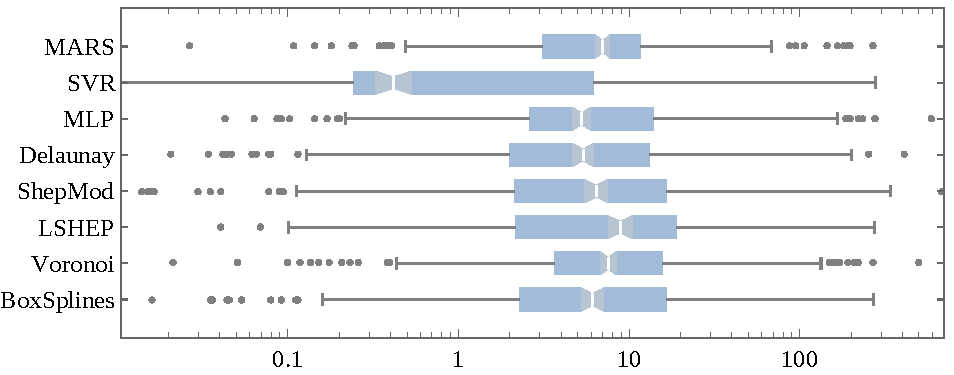
\includegraphics[width=0.9\textwidth,]{Figures/NA/Fig3.pdf}};
    \node[below=of img, node distance=1cm, yshift=1cm] {Number of Data Points};
    \node[left=of img, node distance=0cm, rotate=90, anchor=center,yshift=-0.7cm] {Absolute Error};
  \end{tikzpicture}
  \caption{Delaunay and MLP approximations are constructed from Fekete
    points over the unit cube evaluating the test function $f(x) =
    \cos(\|x\|_2)$ for $x \in \mathbb{R}^{20}$. The details are the
    same as for Fig. \ref{fig:convergence-2d}.}
  \label{fig:convergence-20d}
\end{figure}


The bound from the theorem suggests that by increasing the number of
well-spaced data points, approximation error can be reliably
decreased. The $d = 2$ test seen on the left half of Figure
\ref{fig:convergence-2d} shows a consistent decrease in error for
Delaunay and also shows the eventual accuracy plateau obtained by a
parametric regression form (the MLP, at roughly 500 points). On the
right hand side of Figure \ref{fig:convergence-2d} the random noise
clearly prohibits Delaunay from converging to $f$, while the MLP is
able to improve its approximation with more data points on average.
The convergence result for a very low-dimensional problem like this is
expected.  However, intuition fails for higher dimensional problems.

Figure \ref{fig:convergence-20d} shows the test function with $d = 20$
presents a significantly more challenging approximation problem than
its counterpart in low dimension. The same increase in number of data
points from 32 to 8192 causes no apparent improvement in approximation
for either the noise-free or the noisy problems. Perhaps unexpectedly,
the interpolation technique performs better than the regression
technique on the noisy data (right) in Figure
\ref{fig:convergence-20d}, and worse than the regression technique on
the noise-free data (left). This result emphasizes the relevance of
interpolation for problems in high dimension. It also reveals that the
outcome of MLP regressions can get worse when adding more data points.

\begin{figure}
  \centering
  \begin{tikzpicture}
    \node (img)  {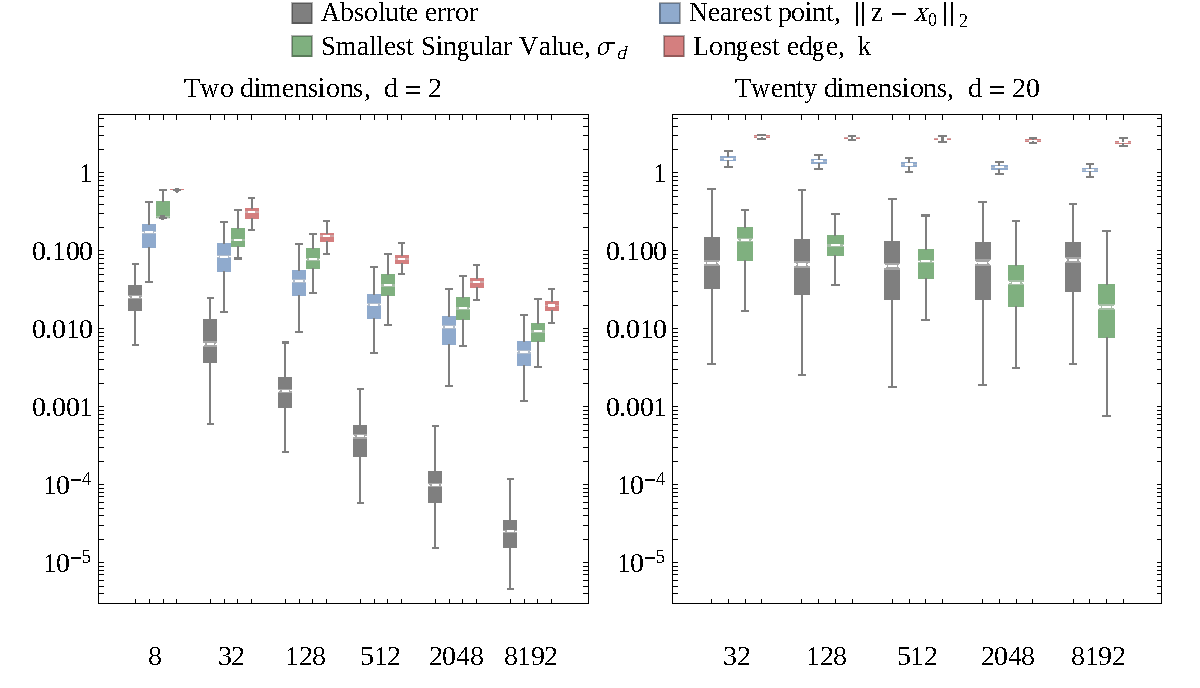
\includegraphics[width=0.9\textwidth,]{Figures/NA/theorem-convergence.pdf}};
    \node[below=of img, node distance=1cm, yshift=1cm] {Number of Data Points};
    \node[left=of img, node distance=0cm, rotate=90, anchor=center,yshift=-0.7cm] {Error, Distance, and Smallest SV };
  \end{tikzpicture}
  \caption{The distribution of absolute error, distance to
    the nearest data point, smallest singular value (SV) and the
    longest edge of the simplex containing each approximation point in
    the tests from Fig. \ref{fig:convergence-2d} and
    Fig. \ref{fig:convergence-20d} for Delaunay. In two dimensions it
    can be seen that $\|z - x_0\|_2$, $\sigma_d$, and $k$ all shrink
    at the same rate for well-spaced approximation points, resulting
    in a faster rate of decrease for approximation error. Notice that
    in higher dimension the data remains sparse even with thousands of
    data points, and the decay in data spacing is more prominant. The
    relatively small reduction in $k$ along with the decrease in
    $\sigma_d$ explain the minimal reduction in error seen by Delaunay
    in Fig. \ref{fig:convergence-20d}.}
  \label{fig:data-spacing}
\end{figure}

The results achieved for both $d = 2$ and $d = 20$ align with the
theoretical error bound as can be seen in Figure
\ref{fig:data-spacing}. In low dimension, thousands of data points
meaningfully reduce the sparsity of the approximation problem.
However, in higher dimension it takes many more points to achieve a
reduction in data sparsity while simultaneously being more difficult
to produce well-conditioned simplices. This evidences the
inherent challenge of data sparsity in high dimension approximation
problems. The analytic results presented are not caused by the chosen
test function, but rather the exponential increase in complexity that
accompanies increased dimension.

In summary, the regime of signal-to-noise ratios that result in
competitively accurate interpolants is greater for moderate to high
dimensional problems due to increased sparsity. Acknowledging the
viability of interpolation for problems of moderate dimension, the
next section will consider real-world problems of similar proportion
(thousands of examples in tens of dimensions).


%% ===================================================================
\vspace{-2mm}
\section{Data and Empirical Analysis}
\label{sec:error_data}

This section extends the comparison of interpolation and regression
algorithms to a sample of real-world problems. Five different data
sets of varying dimension and application are utilized to construct
approximations and compare the accuracy of different techniques.

In the following five subsections the sources and targets of each test
data set are described, as well as challenges and limitations related
to approximating these data. The distribution of response values being
modeled is presented followed by the distribution of approximation
errors for each algorithm. The plots for all five data sets have the
same format.

All five data sets are rescaled such that the domain of approximation
is the unit hypercube. The range of the first four data sets is the
real numbers, while the range of the fifth data set is the space of
cumulative distribution functions. All approximation techniques are
applied to the first four data sets, while only those interpolants
whose approximations are convex combinations of observed data are
applied to the final data set.

All approximations are constructed using $k$-fold cross validation as
described in \cite{kohavi1995study} with $k=10$. This approach
randomly partitions data into $k$ (nearly) equal sized sets. Each
algorithm is then evaluated by constructing an approximation over each
unique union of $k-1$ elements of the partition, making predictions
for points in the remaining element. As a result, each observed data
point is used in the construction of $k-1$ different approximations
and is approximated exactly once. The $k$-fold cross validation method
is data-efficient and provides an unbiased estimate of the expected
prediction error \cite{kohavi1995study}, however it should be noted
that neither this method nor others can provide a universally unbiased
estimator for the variance of prediction error \cite{bengio2004no}.

In addition to the figures displaying approximation results for each
data set, scatter plots of predicted versus actual values
  and tables of accompanying numerical results including
  timings and quartiles of prediction error are located in the
Appendix (Section \ref{sec:appendix}). All of the test data sets
capture underlying functions that are almost certainly stochastic. As
described in Section \ref{sec:introduction}, regression techniques
appear most appropriate for these problems. However, typically data
grows exponentially more sparse with increasing dimension. Given that
sparse data regressors tend towards interpolation and, as demonstrated
in Section \ref{sec:analytic}, interpolants produce similar (if not
identical) results, it is presumed that interpolants are equally
viable approximation techniques on these problems.

%% -------------------------------------------------------------------
\subsection{Forest Fire ($n = 504$, $d = 12$)}

\begin{figure}
  \centering
  \begin{tikzpicture}
    \node (img)  {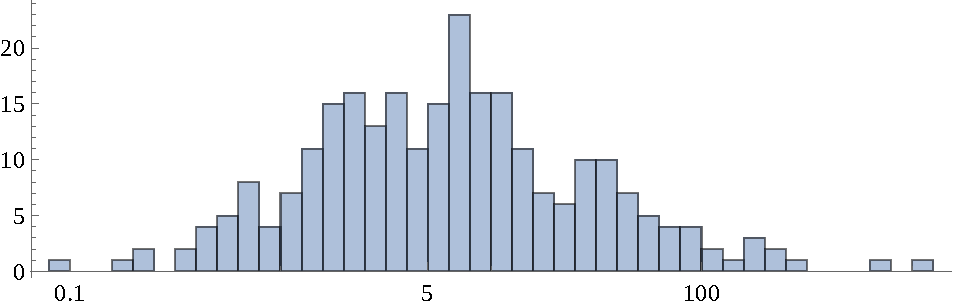
\includegraphics[width=0.75\textwidth,]{Figures/NA/Fig4.pdf}};
    \node[below=of img, node distance=1cm, yshift=1cm] {Forest Fire Area Burned};
    \node[left=of img, node distance=0cm, rotate=90, anchor=center,yshift=-0.7cm] {Count};
  \end{tikzpicture}
  \caption{Histogram of forest fire area burned under recorded weather
    conditions. The data is presented on a $\ln$ scale because
    most values are small with exponentially fewer fires on record
    that burn large areas.}
  \label{fig:hist-forest-fire}

  \vspace{.3cm}

  \begin{tikzpicture}
    \node (img)  {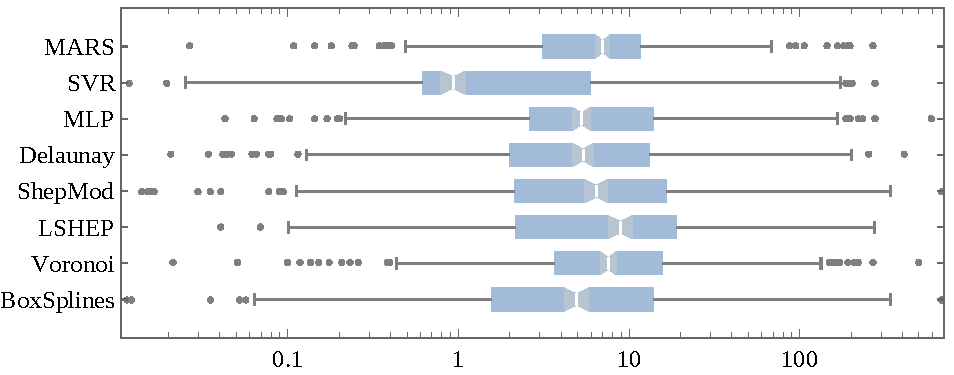
\includegraphics[width=0.8\textwidth,]{Figures/NA/Fig5.pdf}};
    \node[below=of img, node distance=1cm, yshift=1cm] {Area Burned Error};
  \end{tikzpicture}
  \caption{All models are applied to approximate the amount of area
    that would be burned given environment conditions. $10$-fold cross
    validation as described in the beginning of Section \ref{sec:error_data}
    is used to evaluated each algorithm. This results in exactly one
    prediction from each algorithm for each data point. These boxes
    depict the median (middle bar), median $95\%$ confidence interval
    (cones), quartiles (box edges), fences at $3/2$ interquartile
    range (whiskers), and outliers (dots) of absolute prediction error
    for each model. Similar to Figure \ref{fig:hist-forest-fire}, the
    errors are presented on a $\ln$ scale. The numerical data
    corresponding to this figure is provided in Table
    \ref{table:error-forest-fire} in the Appendix.}
  \label{fig:error-forest-fire}
\end{figure}


The forest fire data set \cite{cortez2007data} describes the area of
Montesinho park burned over months of the year along with
environmental conditions. The twelve dimensions being used to model
burn area are the $x$ and $y$ spatial coordinates of burns in the
park, month of year (mapped to $x$, $y$ coordinates on a unit circle),
the FFMC, DMC, DC, and ISI indices (see source for details), the
temperature, relative humidity, wind speed, and outdoor rain. The
original analysis of this data set demonstrated it to be difficult to
model, likely due to the skew in response values.

As suggested by Figure \ref{fig:error-forest-fire}, the SVR has the
lowest absolute prediction errors for $80\%$ of the data, with MLP and
Delaunay being the nearest overall competitors. The effectiveness of
SVR on this data suggests the underlying function can be defined by
relatively few parameters, as well as the importance of capturing the
low-burn-area data points.
%% -------------------------------------------------------------------



%% -------------------------------------------------------------------
\subsection{Parkinson's Telemonitoring ($n = 5875$, $d = 19$)}

\begin{figure}
  \centering
  \begin{tikzpicture}
    \node (img)  {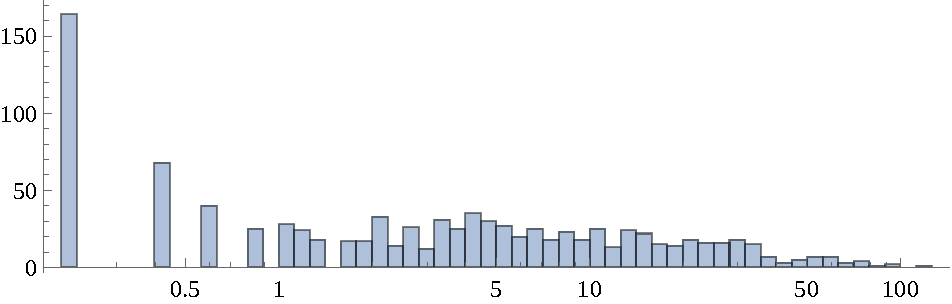
\includegraphics[width=0.75\textwidth,]{Figures/NA/Fig6.pdf}};
    \node[below=of img, node distance=1cm, yshift=1cm] {Parkinson's Total UPDRS Score};
    \node[left=of img, node distance=0cm, rotate=90, anchor=center,yshift=-0.7cm] {Count};
  \end{tikzpicture}
  \caption{Histogram of the Parkinson's patient total UPDRS clinical
    scores that will be approximated by each algorithm.}
  \label{fig:hist-parkinsons}

  \vspace{.3cm}

  \begin{tikzpicture}
    \node (img)  {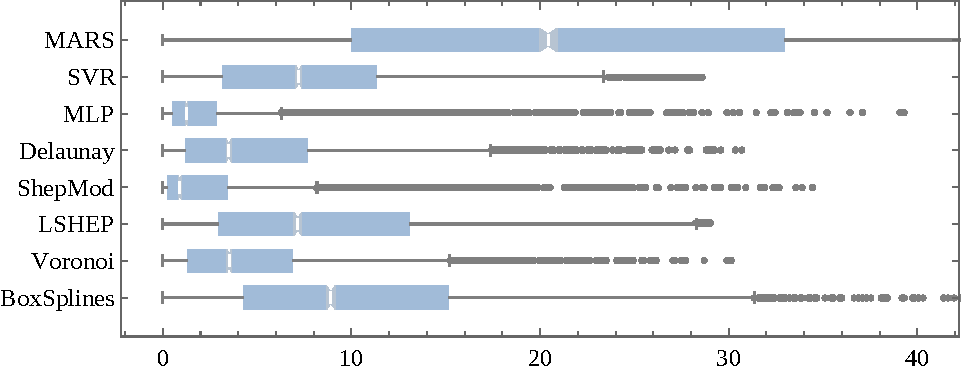
\includegraphics[width=0.8\textwidth,]{Figures/NA/Fig7.pdf}};
    \node[below=of img, node distance=1cm, yshift=1cm] {Total UPDRS Score Error};
  \end{tikzpicture}
  \caption{All models are applied to approximate the total UPDRS score
    given audio features from patients' home life, using $10$-fold
    cross validation. These boxes depict the median (middle bar),
    median $95\%$ confidence interval (cones), quartiles (box edges),
    fences at $3/2$ interquartile range (whiskers), and outliers
    (dots) of absolute prediction error for each model. The numerical
    data corresponding to this figure is provided in Table
    \ref{table:error-parkinsons} in the Appendix.}
  \label{fig:error-parkinsons}
\end{figure}

The second data set for evaluation \cite{tsanas2010accurate} is
derived from a speech monitoring study with the intent to
automatically estimate Parkinson's disease symptom development in
Parkinson's patients. The function to be approximated is a
time-consuming clinical evaluation measure referred to as the UPDRS
score. The total UPDRS score given by a clinical evaluation is
estimated through 19 real numbers generated from biomedical voice
measures of in-home sound recordings.

Figure \ref{fig:error-parkinsons} shows the ShepMod algorithm has the
lowest minimum, first quartile, and median of absolute errors for this
problem, while providing the best prediction $66\%$ of the time. The
MLP has the lowest third quartile and provides the best prediction for
$32\%$ of approximations. The dominance of ShepMod may be due in part
to regular-interval total UPDRS scores provided by clinicians,
favoring a nearest-neighbor strategy of prediction.
%% -------------------------------------------------------------------



%% -------------------------------------------------------------------
\subsection{Australian Daily Rainfall Volume ($n = 2609$, $d = 23$)}

\begin{figure}
  \centering
  \begin{tikzpicture}
    \node (img)  {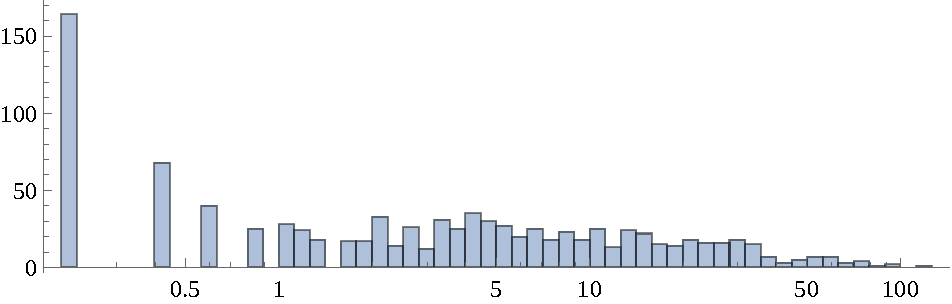
\includegraphics[width=0.75\textwidth,]{Figures/NA/Fig8.pdf}};
    \node[below=of img, node distance=1cm, yshift=1cm] {Daily Rainfall in Sydney};
    \node[left=of img, node distance=0cm, rotate=90, anchor=center,yshift=-0.7cm] {Count};
  \end{tikzpicture}
  \caption{Histogram of daily rainfall in Sydney, Australia, presented
    on a $\ln$ scale because the frequency of larger amounts of
    rainfall is significantly less. There is a peak in occurrence of
    the value $0$, which has a notable effect on the resulting model
    performance.}
  \label{fig:hist-weather}

  \vspace{.3cm}

  \begin{tikzpicture}
    \node (img)  {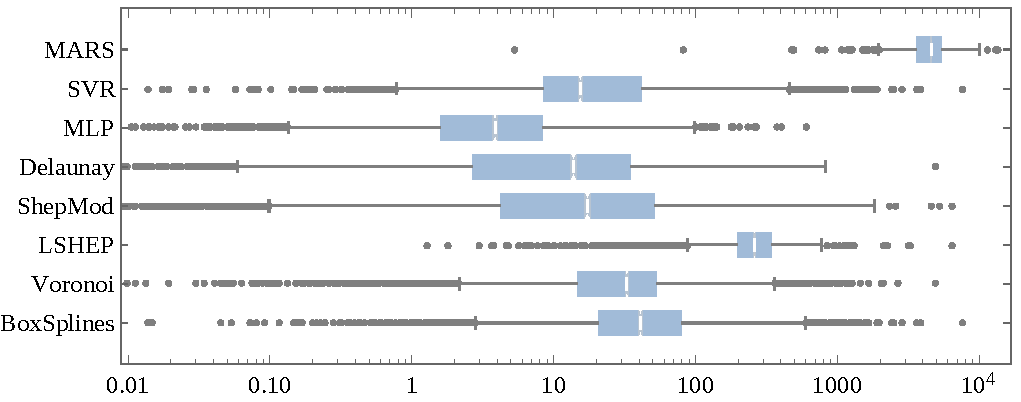
\includegraphics[width=0.8\textwidth,]{Figures/NA/Fig9.pdf}};
    \node[below=of img, node distance=1cm, yshift=1cm] {Sydney Rainfall Tomorrow Error};
  \end{tikzpicture}
  \caption{All models are applied to approximate the amount of
    rainfall expected on the next calendar day given various sources
    of local meteorological data, using $10$-fold cross validation.
    These boxes depict the median (middle bar), median $95\%$
    confidence interval (cones), quartiles (box edges), fences at
    $3/2$ interquartile range (whiskers), and outliers (dots) of
    absolute prediction error for each model. The errors are presented
    on a $\ln$ scale, mimicking the presentation in Figure
    \ref{fig:hist-weather}. The numerical data corresponding to this
    figure is provided in Table \ref{table:error-weather} in the
    Appendix.}
  \label{fig:error-weather}
\end{figure}

The third data set for the total daily rainfall in Sydney, Australia
\cite{williams2009rattle} provides a slightly higher dimensional
challenge for the interpolants and regressors. This data is composed
of many meteorological readings from the region in a day including:
min and max temperatures, sunshine, wind speed directions (converted
to coordinates on a circle), wind speeds, and humidities throughout
the day, day of the year (converted to coordinates on a circle), and
the model must predict the amount of rainfall tomorrow.

While Figure \ref{fig:hist-weather} makes MARS look far better than
other techniques, it only provides the best prediction for $11\%$ of
points. The MLP has the lowest absolute error for $56\%$ of points and
LSHEP is best for $28\%$. MARS likely achieves such a low first
quartile due to the high occurrence of the value zero in the data.
%% -------------------------------------------------------------------



%% -------------------------------------------------------------------
\subsection{Credit Card Transaction Amount ($n = 5562$, $d = 28$)}

\begin{figure}
  \centering
  \begin{tikzpicture}
    \node (img)  {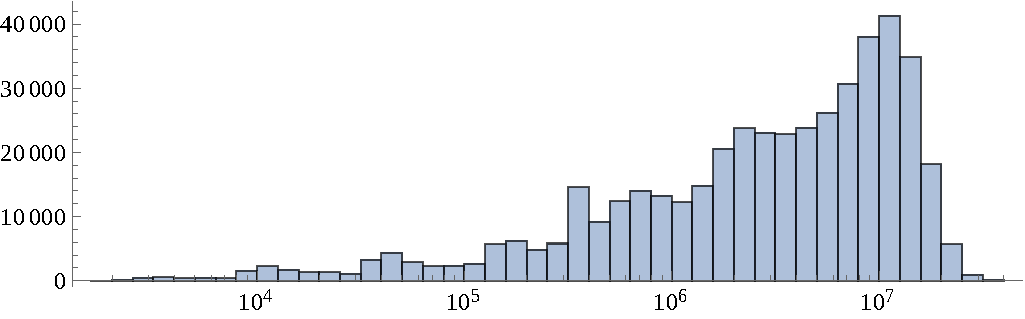
\includegraphics[width=0.75\textwidth,]{Figures/NA/Fig10.pdf}};
    \node[below=of img, node distance=1cm, yshift=1cm] {Credit Card Transaction Amount};
    \node[left=of img, node distance=0cm, rotate=90, anchor=center,yshift=-0.7cm] {Count};
  \end{tikzpicture}
  \caption{Histogram of credit card transaction amounts, presented on
    a $\ln$ scale. The data contains a notable frequency peak around
    $\$1$ transactions. Fewer large purchases are made, but some large
    purchases are in excess of five orders of magnitude greater than
    the smallest purchases.}
  \label{fig:hist-credit-card}

  \vspace{.3cm}

  \begin{tikzpicture}
    \node (img)  {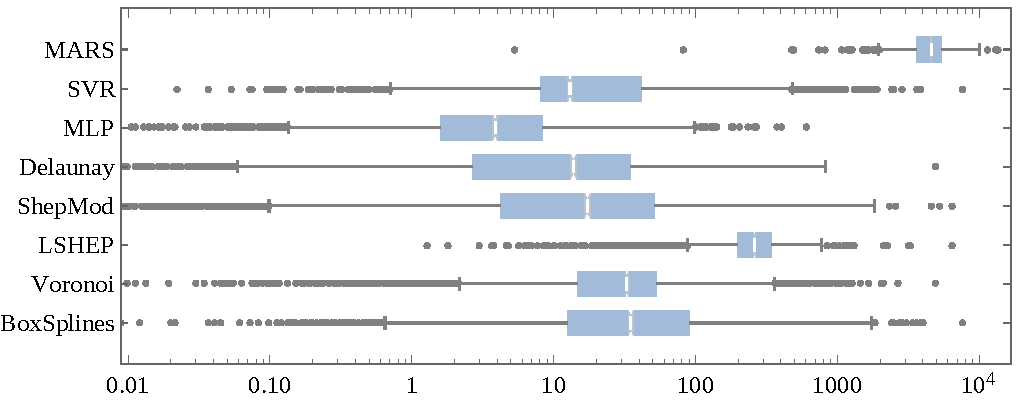
\includegraphics[width=0.8\textwidth,]{Figures/NA/Fig11.pdf}};
    \node[below=of img, node distance=1cm, yshift=1cm] {Transaction Amount Error};
  \end{tikzpicture}
  \caption{All models are applied to approximate the expected
    transaction amount given transformed (and obfuscated) vendor and
    customer-descriptive features, using $10$-fold cross validation.
    These boxes depict the median (middle bar), median $95\%$
    confidence interval (cones), quartiles (box edges), fences at
    $3/2$ interquartile range (whiskers), and outliers (dots) of
    absolute prediction error for each model. The absolute errors in
    transaction amount predictions are presented on a $\ln$ scale,
    just as in Figure \ref{fig:hist-credit-card}. The numerical data
    corresponding to this figure is provided in Table
    \ref{table:error-credit-card} in the Appendix.}
  \label{fig:error-credit-card}
\end{figure}

The fourth test data set, and the final with a real-valued range, is a
collection of credit card transactions
\cite{pozzolo2015calibrating}. The provided data carries no direct
real-world meaning, being the output of a principle component analysis
on the original hidden source data. This obfuscation is done to
protect the information of the credit card users. This data has the
largest dimension of all considered, at 28. A model for this data
predicts the transaction amount given the vector of principle
component information.

As can be seen in Figure \ref{fig:error-credit-card}, the MLP
outperforms all other algorithms at the first, second, third, and
fourth quartiles. The MLP produces the lowest absolute error
prediction for $80\%$ of transactions, Delaunay bests the remaining
$20\%$. It is likely that with less data, Delaunay would be the best
performer.
%% -------------------------------------------------------------------


%% -------------------------------------------------------------------
\subsection{High Performance Computing I/O ($n = 3016$, $d = 4$)}

\begin{figure}
  \centering
  \begin{tikzpicture}
    \node (img)  {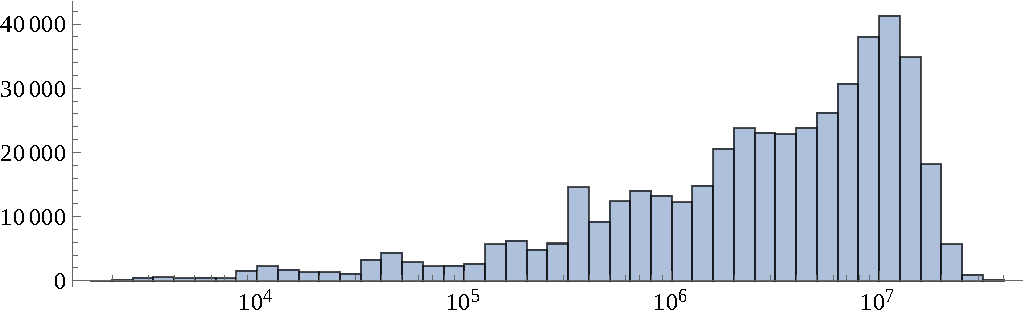
\includegraphics[width=0.75\textwidth,]{Figures/NA/Fig12.pdf}};
    \node[below=of img, node distance=1cm, yshift=1cm] {I/O Read Throughput};
    \node[left=of img, node distance=0cm, rotate=90, anchor=center,yshift=-0.7cm] {Count};
  \end{tikzpicture}
  \caption{Histogram of the raw throughput values recorded during all
    IOzone tests across all system configurations. The distribution is
    skewed right, with few tests having significantly higher
    throughput than most others. The data is presented on a $\ln$
    scale.}
  \label{fig:hist-throughput}
\end{figure}

\begin{figure}
  \centering
  \begin{tikzpicture}
    \node (img)  {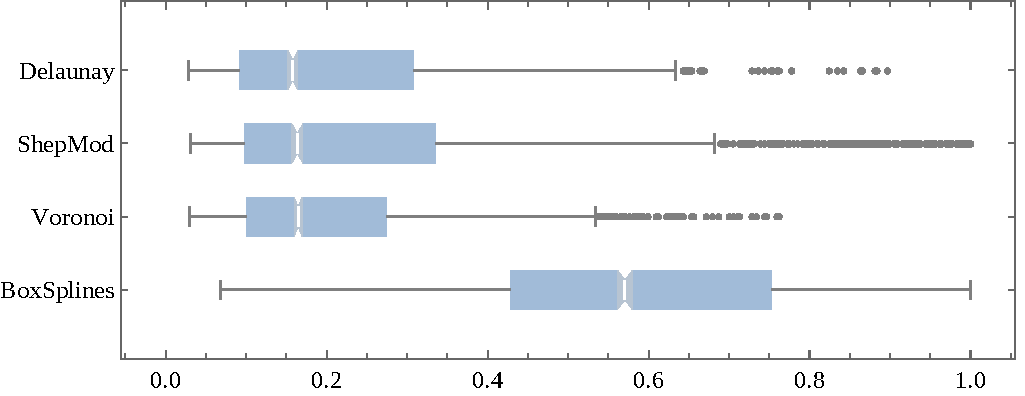
\includegraphics[width=0.8\textwidth,]{Figures/NA/Fig13.pdf}};
    \node[below=of img, node distance=1cm, yshift=1cm] {Read Throughput KS Statistic};
  \end{tikzpicture}
  \caption{The models directly capable of predicting distributions are
    applied to predicting the expected CDF of I/O throughput at a
    previously unseen system configuration, using $10$-fold cross
    validation. The KS statistic (max norm) between the observed
    distribution at each system configuration and the predicted
    distribution is recorded and presented above. Note that the above
    figure is \textit{not} log-scaled like Figure
    \ref{fig:hist-throughput}. The numerical data corresponding to
    this figure is provided in Table \ref{table:error-throughput} in
    the Appendix.}
  \label{fig:error-throughput}
\end{figure}

The final of five data sets is derived from \cite{cameron2019moana},
which provides four-dimensional distribution data by executing the
IOzone benchmark \cite{iozone} on a computer system and varying the
system's file size, record size, thread count, and CPU frequency. At
each configuration, IOzone samples the I/O file-read throughput (in
bytes per second) 150 times. Empirical distribution function points
are computed from each set of 150 executions, which are interpolated
with a piecewise cubic Hermite interpolating polynomial
\cite{fritsch1980monotone} to approximate the CDF. All interpolation
algorithms with the exception of LSHEP are used to approximate these
CDFs from system configurations.

Delaunay achieves the lowest KS statistic (max norm difference) for
$62\%$ of approximations, while Voronoi is best for the remaining
$38\%$. Figure \ref{fig:error-throughput} shows that while Delaunay
may have more best predictions, the behavior of Voronoi may be
preferable.
%% -------------------------------------------------------------------


%% -------------------------------------------------------------------
\begin{figure}
  \centering
  \begin{tikzpicture}
    \node (img)  {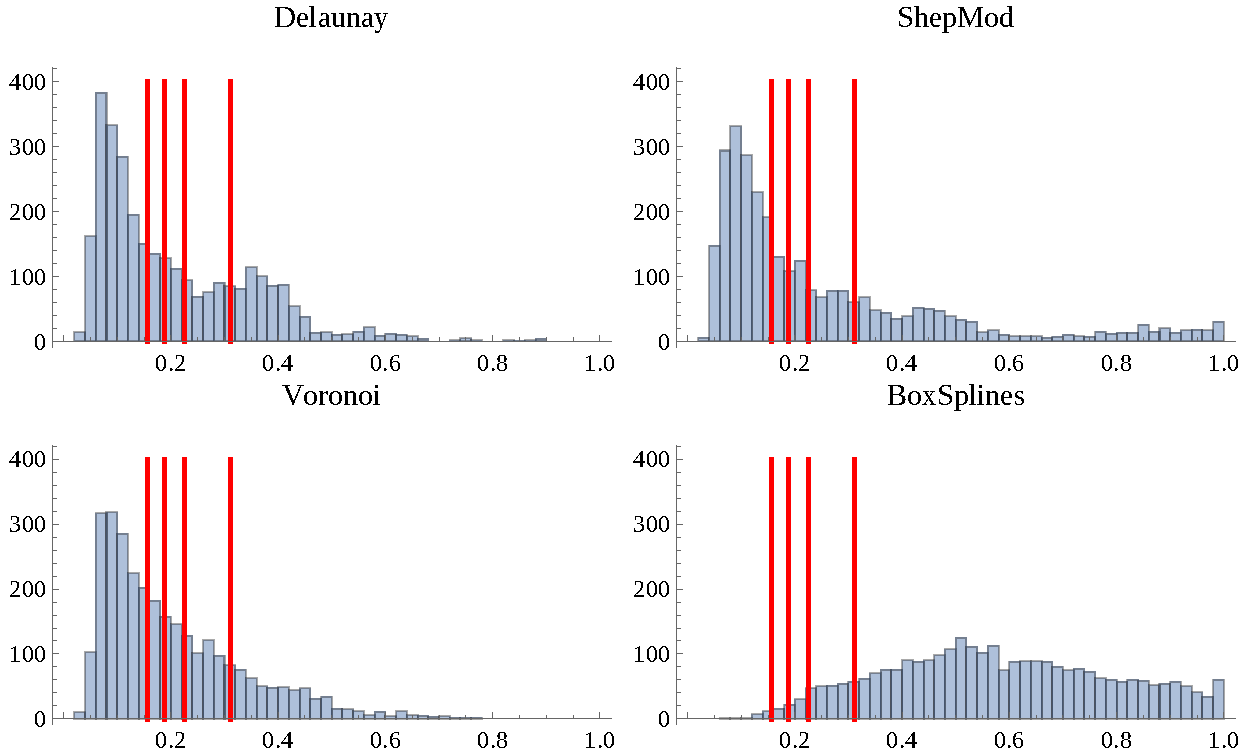
\includegraphics[width=0.8\textwidth]{Figures/NA/Fig14.pdf}};
    \node[below=of img, node distance=1cm, yshift=1cm] {KS Statistic for Predicted vs. Actual};
    \node[left=of img, node distance=0cm, rotate=90, anchor=center,yshift=-0.7cm] {Count of KS Statistic};
  \end{tikzpicture}
  \caption{Histograms of the prediction error for each interpolant
    that produces predictions as convex combinations of observed data,
    using $10$-fold cross validation. The histograms show the KS
    statistics for the predicted throughput distribution versus the
    actual throughput distribution. The four vertical lines represent
    cutoff KS statistics given $150$ samples for commonly used
    $p$-values 0.05, 0.01, 0.001, $10^{-6}$, respectively. All
    predictions to the right of a vertical line represent CDF
    predictions that are significantly different (by respective
    $p$-value) from the actual distribution according to the KS
    test. The numerical counterpart to this figure is presented in
    Table \ref{table:null-hypothesis-results}.}
  \label{fig:throughput-prediction}
\end{figure}

\begin{table}
  \renewcommand{\arraystretch}{1.3}
  \centering
  \begin{tabular}{c|c|c|c|c}
               & $p = .05$         & $p = .01$         & $p = .001$        & $p = 10^{-6}$\\
    \hline
    Delaunay   & $\mathbf{50.3}\%$ & $\mathit{43.5}\%$ & $\mathit{36.2}\%$ & $\mathit{24.7}\%$\\
    ShepMod    & $\mathit{51.4}\%$ & $44.8\%$          & $38.1\%$          & $27.7\%$\\
    Voronoi    & $52.6\%$          & $\mathbf{43.4}\%$ & $\mathbf{34.4}\%$ & $\mathbf{19.1}\%$\\
    BoxSplines & $99.4\%$          & $98.5\%$          & $96.6\%$          & $89.3\%$\\
  \end{tabular}
  \caption{Numerical counterpart of the histogram data presented in
    Figure \ref{fig:throughput-prediction}. The columns display the
    percent of null hypothesis rejections by the KS-test when provided
    different selections of $p$-values for each algorithm. The
    algorithm with the lowest rejection rate at each $p$ is boldface,
    while the second lowest is italicized.}
  \label{table:null-hypothesis-results}
\end{table}


%% ===================================================================

Figure \ref{fig:throughput-prediction} expands on the KS statistic
results presented in Figure \ref{fig:error-throughput}. Agglomerate
errors for each algorithm resemble a Gamma distribution. The
percentages of significant prediction errors with varying $p$-values
are on display in Table \ref{table:null-hypothesis-results}. When
considering the $p=0.001$ results for each technique, a little over
one third of the predicted CDFs are significantly different from the
measured (and presumed) correct CDFs. However, it should be noted that
with 150 samples, the error of an empirical distribution function
(EDF) can reasonably be upwards of $.1$, which serves as a rough
estimate for the lower limit of achievable error. Globally, only a
third of Voronoi predictions fail to capture \textit{all} of the
characteristics of the CDFs at new system configurations.

\section{Discussion of Empirical Results}
\label{sec:discussion}

                                                                      
\begin{table}
  \centering
  \begin{tabular}{c|r@{.}l|r@{.}l|r@{.}l}
    Algorithm & \multicolumn{2}{c|}{Avg. \% Best} & \multicolumn{2}{c|}{\multilinecell{Avg. Fit or \\ Prep. Time (s)}} & \multicolumn{2}{c}{Avg. App. Time (s)}\\
    \hline
    MARS        & \quad\quad$4$&$5$          & \quad\quad$20$&$0$s        & \qquad\quad $0$&$001$s\\
    SVR         & $\mathit{19}$&$\mathit{5}$ & $\mathbf{0}$&$\mathbf{5}$s & $\mathbf{0}$&$\mathbf{0001}$s\\
    MLP         & $\mathbf{43}$&$\mathbf{1}$ & $200$&$0$s                 & $0$&$001$s\\
    Delaunay    & $5$&$2$                    & $1$&$0$s                   & $1$&$0$s\\
    ShepMod     & $18$&$0$                   & $\textit{0}$&$\textit{7}$s & $\mathbf{0}$&$\mathbf{0001}$s\\
    LSHEP       & $8$&$4$                    & $2$&$0$s                   & $\mathbf{0}$&$\mathbf{0001}$s\\
    Voronoi     & $0$&$5$                    & $1$&$0$s                   & $0$&$04$s\\
    BoxSplines  & $3$&$5$                    & $0$&$8$s                   & $\mathit{0}$&$\mathit{0005}$s\\
  \end{tabular}
  \caption{This average of Appendix Tables
    \ref{table:best-forest-fire}, \ref{table:best-parkinsons},
    \ref{table:best-weather}, and \ref{table:best-credit-card}
    provides a gross summary of overall results. The columns display
    (weighted equally by data set, \textit{not} points) the average
    frequency with which any algorithm provided the lowest absolute
    error approximation, the average time to fit/prepare, and the
    average time required to approximate one point. The times have
    been rounded to one significant digit, as reasonably large
    fluctuations may be observed due to implementation hardware.
    Interpolants provide the lowest error approximation for nearly one
    third of all data, while regressors occupy the other two
    thirds. This result is obtained without any customized tuning or
    preprocessing to maximize the performance of any given
    algorithm. In practice, tuning and preprocessing may have large
    effects on approximation performance.}
  \label{table:avg-performance}
\end{table}

Table \ref{table:avg-performance} summarizes results across the four
test data sets with real-valued ranges. The interpolants discussed in
this paper produce the \textit{best} approximations roughly one third
of the time, and produce competitive approximations for almost all
data sets. These test problems are almost certainly
\textit{stochastic} in nature, but the high dimension leads to greater
data sparsity and model construction cost, making interpolation more
competitive.

The major advantages to interpolation lie in the near absence of
\textit{fit} time. Delaunay, LSHEP, and ShepMod all require pairwise
distance calculations, for numerical robustness (Delaunay) and to
determine the radii of influence for data points (LSHEP and
ShepMod). At least hundreds, and sometimes hundreds of thousands of
predictions can be made by the interpolants before the most widely
used regressor (MLP) finishes fitting these relatively small data
sets.  However, the computational complexities of all interpolants
presented are greater than linear in either dimension or number of
points, whereas the regressors' nonlinear complexity in dimension
generally comes from the model fitting optimization.

The new theoretical results presented at the beginning of this chapter
directly apply to Delaunay interpolation, however the performance of
Delaunay does not appear significantly better than other algorithms on
these data sets.  This observation may be due to the stochastic nature
of the data, but it also speaks to the power of the approximations
generated by the different interpolation methods.  The strong
performance of other interpolants suggests that theoretical results
similar to those presented in this work can be achieved for the other
interpolants under reasonable assumptions.

Finally, most of the interpolants presented in this work benefit from
the ability to model \textit{any} function over real $d$-tuples with a
range that is closed under convex combinations. In general, error can
be quantified by any measure (particularly of interest may be
$L^2$, $L^\infty$, etc.). The results of the distribution prediction
case study indicate that interpolants can effectively predict
CDFs. The error analysis for that work relies on the KS statistic,
which captures the worst part of any prediction and hence provides a
conservatively large estimate of approximation error. The average
absolute errors in the predicted CDFs are always lower than the KS
statistics. However, the KS statistic was chosen as a metric because
of the important surrounding statistical theory. A nonnegligible
volume of predictions provide impressively low levels of average
absolute error in that final case study.


\section{Takeaway from Empirical Results}
\label{sec:error_conclusion}

The major contributions of this work are: 1) new uniform theoretical
error bounds for piecewise linear interpolation in arbitrary dimension;
2) an empirical evaluation across
real-world problems that demonstrates interpolants produce
competitively accurate models of multivariate phenomenon when compared
with common regressors for sparse, moderately high dimensional
problems (Section \ref{sec:error_data}); and 3) a demonstration that some
interpolants generalize to interpolation in function spaces, 
preserving monotonicity (with CDFs, e.g.), neither
of which common regressors can do.

The various interpolants discussed in this paper have been
demonstrated to effectively approximate multivariate phenomena up to
$30$ dimensions. The underlying constructions are theoretically
straightforward, interpretable, and yield reasonably accurate
predictions. Most of the interpolants' computational complexities make
them particularly suitable for applications in even higher
dimension. The major benefits of interpolation are seen when only a
small number of approximations ($\leq 1000$) are made from data and
when there are relatively few data points for the dimension (for
empirical results presented, $\log_d n \leq 5$). These findings
encourage broader application of interpolants to multivariate
approximation in science.





%% Propose new method to improve predictions for distributions.
\chapter{Improving Variability Estimates with Monotone $C^2$ Splines} \label{ch:splines}

Many domains of science rely on smooth approximations to real-valued functions over a closed interval. These smooth approximations are regularly used in automotive and aerospace engineering, architecture, mathematics and especially statistics \cite{knott2012interpolating}. While polynomial interpolants or regressors apply broadly, piecewise polynomial functions (splines) are often a good choice because they can approximate globally complex functions while minimizing local complexity of the approximation. It is often the case that the true underlying function or phenomenon being modeled has known properties e.g., convexity, positivity, various levels of continuity, or monotonicity. Given a reasonably large amount of data, it can be impossible to maintain these properties with a single polynomial function.

In general, the maintenance of function properties through interpolation / regression is usually referred to as \textit{shape preserving} \cite{fritsch1980monotone,gregory1985shape}. The specific shapes this work will focus on are monotonicity and multiple levels of continuity for a function. These properties are chiefly important to the approximation of cumulative distribution functions and subsequently the effective generation of random numbers from a specified distribution. 

In statistics especially, the construction of a monotone interpolating spline that is continuous in second derivative is meaningfully useful \cite{ramsay1988monotone}. A function with these properties could approximate random variables to a high level of accuracy with relatively few intervals (with even more accuracy given greater continuity). A continuously twice differentiable approximation to a cumulative distribution function would also produce a corresponding probability density function that is continuously differentiable, which is a property many commonly occurring parametric distributions maintain.


\section{Related Work}

The current state-of-the-art monotone interpolating spline with a mathematical software implementation is piecewise cubic, continuously differentiable, and was first proposed in \citet{fritsch1980monotone} then expanded upon in \citet{carlson1985monotone}. Let $\pi: a = x_1 < x_2 < \cdots < x_n = b$ be a partition of the interval $[a,b]$. Let $\{f(x_i) : i = 1,2,\ldots,n\}$ be a given set of data values at the partition points for a monotone function $f$, meaning $f(x_i) \leq f(x_{i+1})$ for $i = 1, \ldots, n-1$ or $f(x_i) \geq f(x_{i+1})$ for $i = 1, \ldots, n-1$. Let $\hat f$ be a piecewise cubic spline defined in each sub-interval $I_i = [x_i, x_{i+1}]$ by

\begin{align*}
h_i =& \ x_{i+1} - x_{i} \\
u(t) =& \ 3t^2 - 2t^3 \\
p(t) =& \ t^3 - t^2 \\
\hat f(x) =& \ f(x_i)\ u\big((x_{i+1} - x) / h_i\big) + f(x_{i+1})\ u\big((x - x_i) / h_i\big) \\
& - \hat f^{\ \prime}(x_i)\ p\big((x_{i+1}-x)/h_i\big) + \hat f^{\ \prime}(x_{i+1})\ p\big((x-x_i)/h_i \big).
\end{align*}

Notice that it is up to the user to choose values for $\hat f^{\ \prime}$and a viable monotonic cubic spline can be produced by choosing $\hat f^{\ \prime}(x_i) = 0$, $i = 1, \ldots, n$. However, such a spline has too many \textit{wiggles} for most applications. Fritsch and Carlson proceed to show that simple conditions on the derivative values can guarantee monotonicity, and that these conditions can be enforced in a way that ensures modifications on one interval will not break the monotonicity of cubic polynomials over any neighboring intervals. Consider the terms $\alpha = \frac{\hat f^{\ \prime}(x_i) (x_{i+1}-x_i)}{f(x_{i+1}) - f(x_i)}$ and $\beta = \frac{\hat f^{\ \prime}(x_{i+1}) (x_{i+1}-x_i)}{f(x_{i+1}) - f(x_i)}$, now monotonicity of a cubic polynomial over a sub-interval can be maintained by ensuring that $\alpha$ and $\beta$ reside in any of the following regions.

\begin{figure}[htb]
  \centering
  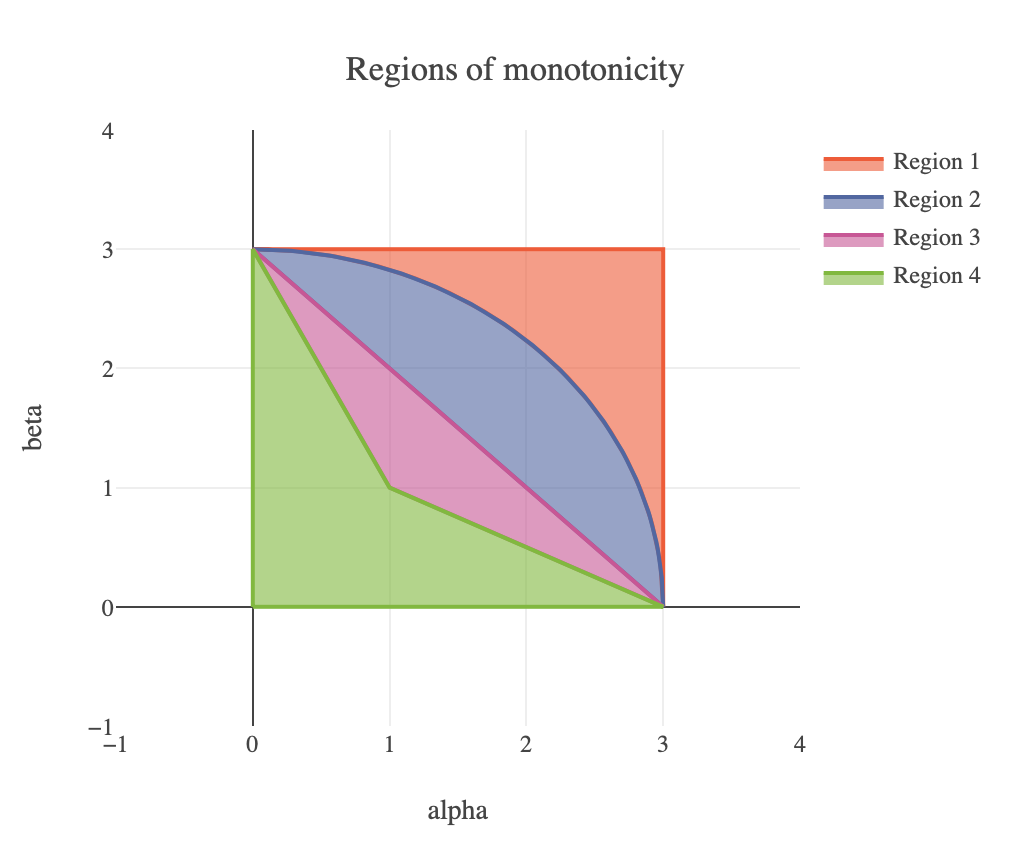
\includegraphics[scale=0.5]{Figures/splines/feasible_region.png}
  \caption{These are the feasible regions of monotonicity for cubic splines.}
  \label{fig:feasible_region}
\end{figure}

The actual region of monotonicity for a cubic polynomial is larger, but projection of $(\alpha, \beta)$ into one of these regions ensures that monotonicity will be achieved and not violated for neighboring regions. The user must decide which region is most suitable to project $(\alpha, \beta)$ onto, Fritsch and Carlson recommend using region 2.

This theoretical work has been extended in \cite{ulrich1994positivity,hess1994positive} to monotone quintic polynomials, but no mathematical software has been produced accordingly. That is where this proposed work comes in.


\section{Achieved Progress}

To expand my own understanding of the current state-of-the-art method for constructing a monotone spline interpolant, I \href{https://github.com/tchlux/VarSys/blob/master/Disseration/cubic.py}{fully implemented} the algorithm described in \cite{fritsch1980monotone} in Python. This code can be used to generate monotone cubic spline fits to data and allows for the user specification of a method((the means by which monotonicity is enforced)) and derivatives at any of the knots or endpoints. Clearly this code is not optimized for numerical robustness, nor speed, but it serves as a portable demonstration and educational tool.

Here we can see the recommended method of projection for moving cubic polynomials into the region of monotonicity.

\begin{figure}[htb]
  \centering
  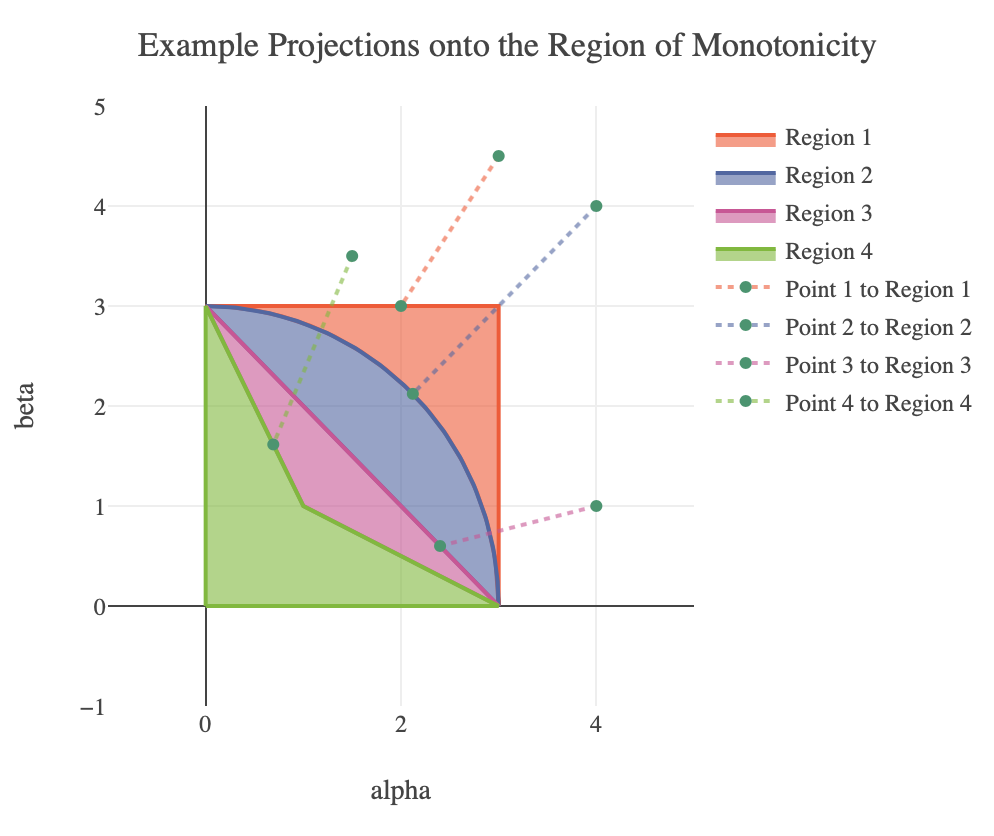
\includegraphics[scale=0.5]{Figures/splines/demo_projection.png}
  \caption{A demonstration of projection onto the feasible region for cubic splines.}
  \label{fig:demo_projection}
\end{figure}

The resulting interpolating spline is $C^1$ and has a \textit{smooth} appearance, here is a demonstration when using Region 2.

\begin{figure}[htb]
  \centering
  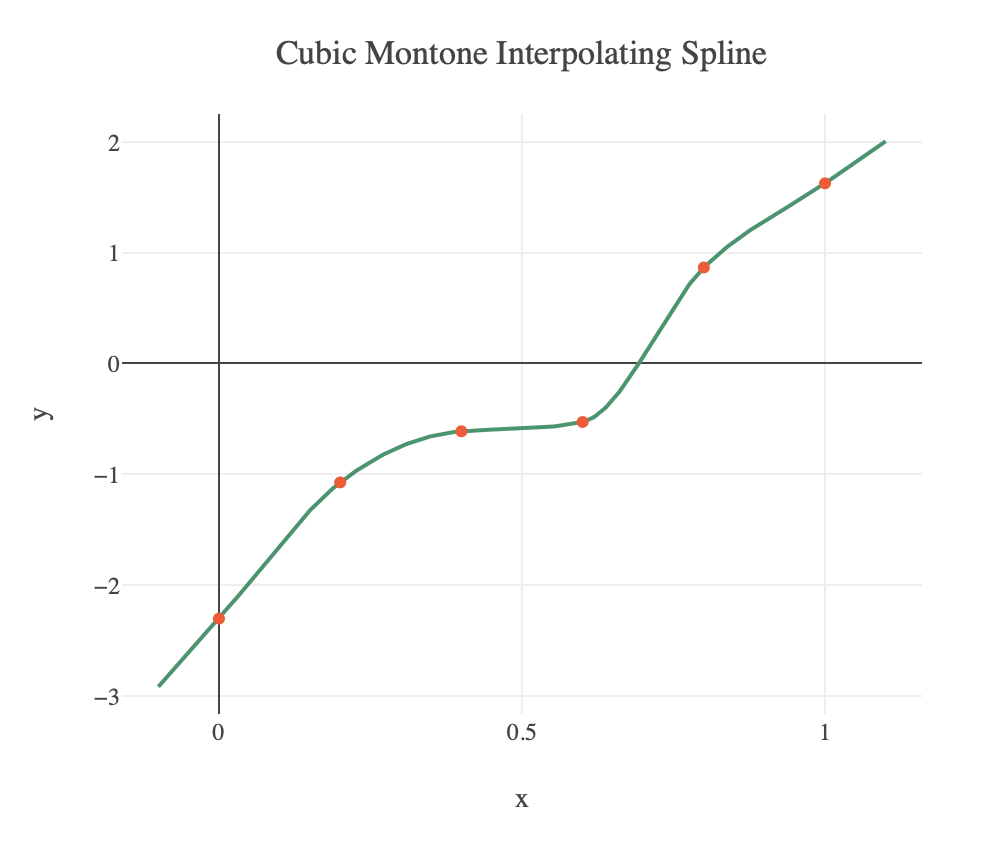
\includegraphics[scale=0.5]{Figures/splines/demo_fit.png}
  \caption{A demonstration fit with a cubic spline.}
  \label{fig:demo_fit}
\end{figure}

And the derivative of the above spline is continuous.

\begin{figure}[htb]
  \centering
  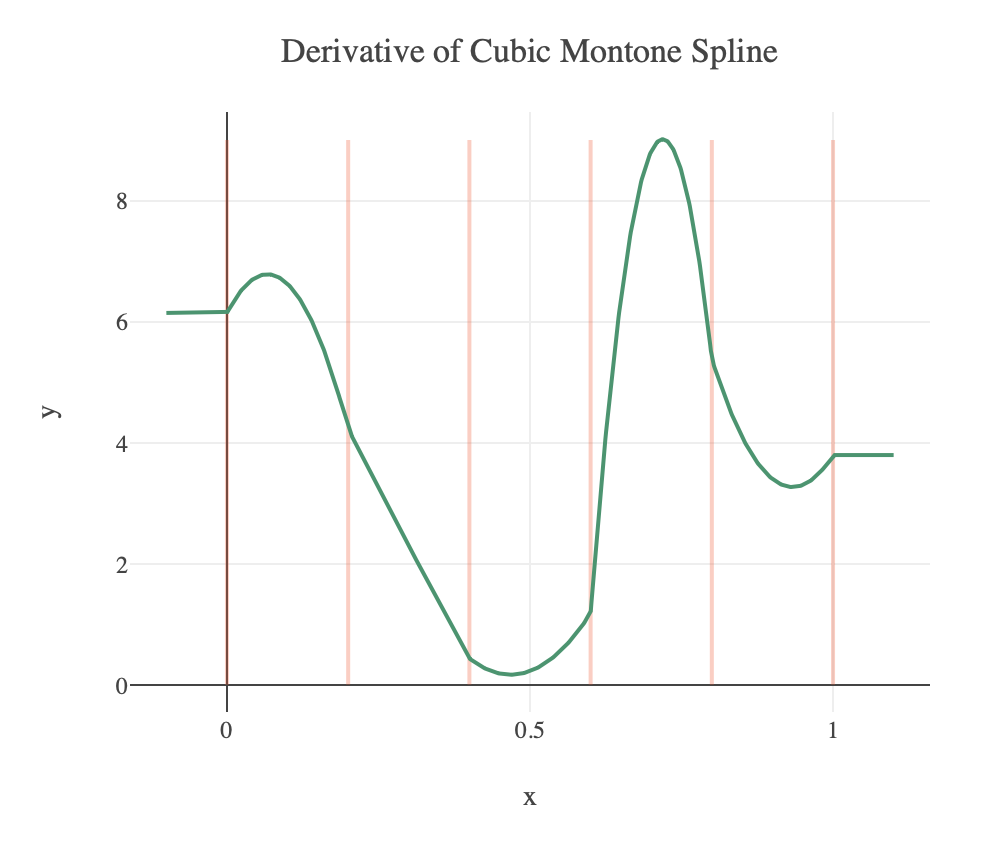
\includegraphics[scale=0.5]{./Figures/splines/demo_fit_deriv.png}
  \caption{The derivative of Figure \ref{fig:demo_projection}.}
  \label{fig:demo_fit_deriv}
\end{figure}

\section{Research Goal}

{\centering \textbf{Produce numerically robust software that computes monotone quintic interpolating splines given data.}}

\section{Timeline}

The projected research timeline is shown in Table \ref{tab:timeline}. It is expected that a significant number of \textit{unpredictable changes} will occur as the code develops and the research progresses. I will update all committee members when appropriate.

\begin{table}
  \centering
  \renewcommand{\arraystretch}{1.2}
  \begin{tabular}{l l}
    \textbf{Date} & \textbf{Milestone} \\ \hline
    \textit{June 2019} & Implementation of monotone quintic polynomial \textit{interpolant}. \\
    \textit{August 2019} & Implementation of monotone quintic polynomial \textit{spline}. \\
    \textit{October 2019} & First draft of TOMS paper on algorithm. \\
    \textit{December 2019} & Research Defense of work. \\
    \textit{March 2020} & Submission of TOMS paper and code. \\
    \textit{April 2020} & Final Defense of Ph.D.
  \end{tabular}
  \caption{This table depicts my expected timeline going forward. For details on when I achieved previous milestones, please contact me and I can provide the list. I refrained from including it here for brevity.}
  \label{tab:timeline}
\end{table}

\section{Final Remarks}

This project has the potential to be very widely utilized. As described earlier, many statistical applications could greatly benefit from having a $C^2$ approximation to CDFs, because the resulting PDF will be both aesthetically pleasing and more accurate for continuous distributions.




%% Bibliography.
\bibliography{prelim}
\bibliographystyle{plainnat}


% This formats the chapter name to appendix to properly define the headers:
\appendix

% Add your appendices here. You must leave the appendices enclosed in the appendices environment in order for the table of contents to be correct.
\begin{appendices}
  \chapter{Error Bound Appendices} \label{app:error}

  The tables that follow show the precise experimental results for all
  data sets presented in Section \ref{sec:data}. The tests were all run
  serially on an otherwise idle machine with a CentOS 6.10 operating
  system and an Intel i7-3770 CPU operating at 3.4 GHz. The detailed
  performance results in the tables that follow are very much dependent
  on the problem and the algorithm implementation (e.g., some codes are
  TOMS software, some industry distributions, and others are from
  conference paper venues). Different typeface is used to show best
  performers, however not much significance should be attached to
  ranking algorithms based on small time (millisecond) differences. The
  results serve as a demonstration of conceptual validity.

  \begin{table}[H]
    \centering
    \begin{tabular}{c|r@{.}l|r@{.}l|r@{.}l|r@{.}l|r@{.}l}
      \hline
      Algorithm & \multicolumn{2}{c|}{Min} & \multicolumn{2}{c|}{$25^{th}$} & \multicolumn{2}{c|}{$50^{th}$} & \multicolumn{2}{c|}{$75^{th}$} & \multicolumn{2}{c}{Max}\\
      \hline
      MARS & $0$&$00984$ & $3$&$11$ & $7$&$01$ & $\mathit{11}$&$\mathit{7}$ & $1090$&$0$\\
      SVR & $\mathit{0}$&$\mathit{00402}$ & $\mathbf{0}$&$\mathbf{243}$ & $\mathbf{0}$&$\mathbf{416}$ & $\mathbf{6}$&$\mathbf{19}$ & $1090$&$0$\\
      MLP & $0$&$0426$ & $2$&$63$ & $\mathit{5}$&$\mathit{27}$ & $14$&$0$ & $1090$&$0$\\
      Delaunay & $\mathbf{0}$&$\mathbf{00}$ & $1$&$98$ & $5$&$37$ & $13$&$1$ & $\mathit{1080}$&$\mathit{0}$\\
      ShepMod & $\mathbf{0}$&$\mathbf{00}$ & $\mathit{1}$&$\mathit{93}$ & $6$&$27$ & $16$&$0$ & $1090$&$0$\\
      LSHEP & $0$&$0400$ & $2$&$17$ & $8$&$87$ & $19$&$1$ & $\mathbf{1070}$&$\mathbf{0}$\\
      Voronoi & $0$&$00982$ & $3$&$65$ & $7$&$56$ & $15$&$6$ & $1090$&$0$\\
      BoxSpline & $\mathbf{0}$&$\mathbf{00}$ & $2$&$27$ & $5$&$91$ & $16$&$4$ & $1090$&$0$\\
      \hline
    \end{tabular}
    \caption{This numerical data accompanies the visual provided in
      Figure \ref{fig:error-forest-fire}. The columns of absolute error
      percentiles correspond to the minimum, first quartile, median,
      third quartile, and maximum absolute errors respectively. The
      minimum of each column is boldface, while the second lowest value
      is italicized. All values are rounded to three significant
      digits.}
    \label{table:error-forest-fire}
  \end{table}

  \begin{table}[H]
    \centering
    \begin{tabular}{|c|r@{.}l| c |r@{.}l|r@{.}l|r@{.}l|}
      \cline{1-3}\cline{5-10}
      Algorithm & \multicolumn{2}{c|}{\% Best} &  & \multicolumn{2}{c|}{Fit/Prep. Time (s)} & \multicolumn{2}{c|}{App. Time (s)} & \multicolumn{2}{c|}{Total App. Time (s)}\\
      \cline{1-3}\cline{5-10}
      MARS & \quad$\mathit{7}$&$\mathit{7}$ &  & \quad\quad$29$&$1$ & \quad$0$&$00137$ & \quad\quad\quad$0$&$0686$\\
      SVR & $\mathbf{80}$&$\mathbf{2}$ &  & $\mathbf{0}$&$\mathbf{00584}$ & $\mathit{0}$&$\mathit{0000620}$ & $\mathit{0}$&$\mathit{00310}$\\
      MLP & $0$&$0$ &  & $32$&$8$ & $0$&$000871$ & $0$&$0436$\\
      Delaunay & $3$&$5$ &  & $0$&$0151$ & $0$&$0234$ & $1$&$18$\\
      ShepMod & $3$&$7$ &  & $\mathit{0}$&$\mathit{00634}$ & $0$&$0000644$ & $0$&$00322$\\
      LSHEP & $5$&$1$ &  & $0$&$0275$ & $\mathbf{0}$&$\mathbf{0000463}$ & $\mathbf{0}$&$\mathbf{00231}$\\
      Voronoi & $0$&$0$ &  & $0$&$0152$ & $0$&$000396$ & $0$&$0198$\\
      BoxSpline & $0$&$4$ &  & $0$&$00724$ & $0$&$0000978$ & $0$&$00489$\\
      \cline{1-3}\cline{5-10}
    \end{tabular}
    \caption{The left above shows how often each algorithm had the
      lowest absolute error approximating forest fire data in Table
      \ref{table:error-forest-fire}. On the right columns are median fit
      time of 454 points, median time for one approximation, and median
      time approximating 50 points.}
    \label{table:best-forest-fire}
  \end{table}

  \begin{table}
    \centering
    \begin{tabular}{c|r@{.}l|r@{.}l|r@{.}l|r@{.}l|r@{.}l}
      \hline
      Algorithm & \multicolumn{2}{c|}{Min} & \multicolumn{2}{c|}{$25^{th}$} & \multicolumn{2}{c|}{$50^{th}$} & \multicolumn{2}{c|}{$75^{th}$} & \multicolumn{2}{c}{Max}\\
      \hline
      MARS & $0$&$00948$ & $9$&$98$ & $20$&$4$ & $32$&$9$ & $863$&$0$\\
      SVR & $0$&$00138$ & $3$&$17$ & $7$&$31$ & $12$&$6$ & $\mathbf{27}$&$\mathbf{5}$\\
      MLP & $0$&$0000239$ & $\mathit{0}$&$\mathit{533}$ & $\mathit{1}$&$\mathit{25}$ & $\mathbf{2}$&$\mathbf{84}$ & $39$&$3$\\
      Delaunay & $\mathit{3}$&$\mathit{72 \times 10^{-12}}$ & $1$&$20$ & $3$&$50$ & $7$&$67$ & $30$&$7$\\
      ShepMod & $\mathbf{0}$&$\mathbf{0}$ & $\mathbf{0}$&$\mathbf{255}$ & $\mathbf{0}$&$\mathbf{908}$ & $\mathit{3}$&$\mathit{43}$ & $34$&$5$\\
      LSHEP & $0$&$00254$ & $2$&$93$ & $7$&$16$ & $13$&$1$ & $\mathit{29}$&$\mathit{0}$\\
      Voronoi & $\mathbf{0}$&$\mathbf{0}$ & $1$&$29$ & $3$&$52$ & $6$&$87$ & $30$&$1$\\
      BoxSpline & $0$&$00287$ & $4$&$39$ & $9$&$10$ & $14$&$8$ & $41$&$3$\\
      \hline
    \end{tabular}
    \caption{This numerical data accompanies the visual provided in
      Figure \ref{fig:error-parkinsons}. The columns of absolute error
      percentiles correspond to the minimum, first quartile, median,
      third quartile, and maximum absolute errors respectively. The
      minimum of each column is boldface, while the second lowest value
      is italicized. All values are rounded to three significant
      digits.}
    \label{table:error-parkinsons}
  \end{table}

  \begin{table}
    \centering
    \begin{tabular}{|c|r@{.}l| c |r@{.}l|r@{.}l|r@{.}l|}
      \cline{1-3}\cline{5-10}
      Algorithm & \multicolumn{2}{c|}{\% Best} &  & \multicolumn{2}{c|}{Fit/Prep. Time (s)} & \multicolumn{2}{c|}{App. Time (s)} & \multicolumn{2}{c|}{Total App. Time (s)}\\
      \cline{1-3}\cline{5-10}
      MARS & \quad\,$0$&$0$ &  & \quad\quad\quad$37$&$9$ & \quad\,\,$0$&$00253$ & \quad\quad\quad\,\,$1$&$48$\\
      SVR & $0$&$1$ &  & $\mathbf{0}$&$\mathbf{859}$ & $\mathit{0}$&$\mathit{000181}$ & $\mathit{0}$&$\mathit{106}$\\
      MLP & $\mathit{32}$&$\mathit{0}$ &  & $348$&$0$ & $0$&$00111$ & $0$&$653$\\
      Delaunay & $0$&$0$ &  & $2$&$47$ & $1$&$22$ & $720$&$0$\\
      ShepMod & $\mathbf{66}$&$\mathbf{4}$ &  & $\mathit{1}$&$\mathit{13}$ & $0$&$000182$ & $0$&$107$\\
      LSHEP & $0$&$0$ &  & $2$&$39$ & $\mathbf{0}$&$\mathbf{000144}$ & $\mathbf{0}$&$\mathbf{0845}$\\
      Voronoi & $1$&$6$ &  & $2$&$77$ & $0$&$0274$ & $16$&$1$\\
      BoxSpline & $0$&$0$ &  & $1$&$26$ & $0$&$000643$ & $0$&$377$\\
      \cline{1-3}\cline{5-10}
    \end{tabular}
    \caption{The left above shows how often each algorithm had the
      lowest absolute error approximating Parkinson's data in Table
      \ref{table:error-parkinsons}. On the right columns are median fit
      time of 5288 points, median time for one approximation, and median
      time approximating 587 points.}
    \label{table:best-parkinsons}
  \end{table}


  \begin{table}
    \centering
    \begin{tabular}{c|r@{.}l|r@{.}l|r@{.}l|r@{.}l|r@{.}l}
      \hline
      Algorithm & \multicolumn{2}{c|}{Min} & \multicolumn{2}{c|}{$25^{th}$} & \multicolumn{2}{c|}{$50^{th}$} & \multicolumn{2}{c|}{$75^{th}$} & \multicolumn{2}{c}{Max}\\
      \hline
      MARS & $\mathit{6}$&$\mathit{45 \times 10^{-15}}$ & $\mathbf{2}$&$\mathbf{70 \times 10^{-14}}$ & $1$&$66$ & $1$&$96$ & $\mathit{53}$&$\mathit{3}$\\
      SVR & $0$&$0420$ & $0$&$143$ & $0$&$148$ & $\mathit{0}$&$\mathit{860}$ & $119$&$0$\\
      MLP & $0$&$0000689$ & $0$&$0337$ & $\mathbf{0}$&$\mathbf{0795}$ & $\mathbf{0}$&$\mathbf{264}$ & $\mathbf{5}$&$\mathbf{31}$\\
      Delaunay & $\mathbf{0}$&$\mathbf{0}$ & $0$&$187$ & $0$&$919$ & $2$&$72$ & $56$&$3$\\
      ShepMod & $\mathbf{0}$&$\mathbf{0}$ & $0$&$0957$ & $0$&$685$ & $2$&$90$ & $73$&$2$\\
      LSHEP & $\mathbf{0}$&$\mathbf{0}$ & $\mathit{0}$&$\mathit{0153}$ & $\mathit{0}$&$\mathit{106}$ & $1$&$17$ & $113$&$0$\\
      Voronoi & $\mathbf{0}$&$\mathbf{0}$ & $0$&$430$ & $1$&$28$ & $2$&$94$ & $83$&$8$\\
      BoxSpline & $\mathbf{0}$&$\mathbf{0}$ & $0$&$789$ & $2$&$06$ & $5$&$25$ & $119$&$0$\\
      \hline
    \end{tabular}
    \caption{This numerical data accompanies the visual provided in
      Figure \ref{fig:error-weather}. The columns of absolute error
      percentiles correspond to the minimum, first quartile, median,
      third quartile, and maximum absolute errors respectively. The
      minimum value of each column is boldface, while the second lowest
      is italicized. All values are rounded to three significant
      digits.}
    \label{table:error-weather}
  \end{table}

  \begin{table}
    \centering
    \begin{tabular}{|c|r@{.}l| c |r@{.}l|r@{.}l|r@{.}l|}
      \cline{1-3}\cline{5-10}
      Algorithm & \multicolumn{2}{c|}{\% Best} &  & \multicolumn{2}{c|}{Fit/Prep. Time (s)} & \multicolumn{2}{c|}{App. Time (s)} & \multicolumn{2}{c|}{Total App. Time (s)}\\
      \cline{1-3}\cline{5-10}
      MARS & \,\,\,\,$10$&$7$ &  & \quad\quad\quad$\mathit{0}$&$\mathit{151}$ & \quad$0$&$000117$ & \quad\quad\quad\,\,$0$&$0304$\\
      SVR & $4$&$1$ &  & $\mathbf{0}$&$\mathbf{133}$ & $\mathbf{0}$&$\mathbf{0000947}$ & $\mathbf{0}$&$\mathbf{0246}$\\
      MLP & $\mathbf{56}$&$\mathbf{8}$ &  & $169$&$0$ & $0$&$00137$ & $0$&$356$\\
      Delaunay & $0$&$1$ &  & $0$&$664$ & $0$&$886$ & $230$&$0$\\
      ShepMod & $3$&$5$ &  & $0$&$265$ & $0$&$000128$ & $0$&$0333$\\
      LSHEP & $\mathit{28}$&$\mathit{4}$ &  & $0$&$874$ & $\mathit{0}$&$\mathit{0000975}$ & $\mathit{0}$&$\mathit{0254}$\\
      Voronoi & $0$&$2$ &  & $0$&$675$ & $0$&$0270$ & $7$&$01$\\
      BoxSpline & $0$&$3$ &  & $0$&$330$ & $0$&$000406$ & $0$&$106$\\
      \cline{1-3}\cline{5-10}
    \end{tabular}
    \caption{Left table shows how often each algorithm had the lowest
      absolute error approximating Sydney rainfall data in Table
      \ref{table:error-weather}. On the right columns are median fit
      time of 2349 points, median time for one approximation, and median
      time approximating 260 points.}
    \label{table:best-weather}
  \end{table}


  \begin{table}
    \centering
    \begin{tabular}{c|r@{.}l|r@{.}l|r@{.}l|r@{.}l|r@{.}l}
      \hline
      Algorithm & \multicolumn{2}{c|}{Min} & \multicolumn{2}{c|}{$25^{th}$} & \multicolumn{2}{c|}{$50^{th}$} & \multicolumn{2}{c|}{$75^{th}$} & \multicolumn{2}{c}{Max}\\
      \hline
      MARS & $5$&$36$ & $3610$&$0$ & $4580$&$0$ & $5450$&$0$ & $13400$&$0$\\
      SVR & $0$&$0138$ & $8$&$47$ & $15$&$4$ & $41$&$9$ & $7700$&$0$\\
      MLP & $0$&$00151$ & $\mathbf{1}$&$\mathbf{60}$ & $\mathbf{3}$&$\mathbf{86}$ & $\mathbf{8}$&$\mathbf{34}$ & $\mathbf{604}$&$\mathbf{0}$\\
      Delaunay & $\mathbf{0}$&$\mathbf{0}$ & $\mathit{2}$&$\mathit{69}$ & $\mathit{13}$&$\mathit{8}$ & $\mathit{35}$&$\mathit{0}$ & $\mathit{4840}$&$\mathit{0}$\\
      ShepMod & $\mathbf{0}$&$\mathbf{0}$ & $4$&$21$ & $17$&$3$ & $51$&$6$ & $6510$&$0$\\
      LSHEP & $1$&$27$ & $199$&$0$ & $260$&$0$ & $343$&$0$ & $6530$&$0$\\
      Voronoi & $\mathit{2}$&$\mathit{89 \times 10^{-10}}$ & $14$&$7$ & $32$&$8$ & $52$&$9$ & $4860$&$0$\\
      BoxSpline & $0$&$00740$ & $20$&$8$ & $40$&$9$ & $79$&$6$ & $7640$&$0$\\
      \hline
    \end{tabular}
    \caption{This numerical data accompanies the visual provided in
      Figure \ref{fig:error-credit-card}. The columns of absolute error
      percentiles correspond to the minimum, first quartile, median,
      third quartile, and maximum absolute errors respectively. The
      minimum value of each column is boldface, while the second lowest
      is italicized. All values are rounded to three significant
      digits.}
    \label{table:error-credit-card}
  \end{table}

  \begin{table}
    \centering
    \begin{tabular}{|c|r@{.}l| c |r@{.}l|r@{.}l|r@{.}l|}
      \cline{1-3}\cline{5-10}
      Algorithm & \multicolumn{2}{c|}{\% Best} &  & \multicolumn{2}{c|}{Fit/Prep. Time (s)} & \multicolumn{2}{c|}{App. Time (s)} & \multicolumn{2}{c|}{Total App. Time (s)}\\
      \cline{1-3}\cline{5-10}
      MARS & \quad\,$0$&$0$ &  & \quad\quad\quad$22$&$0$ & \quad$0$&$00148$ & \quad\quad\quad\,\,$0$&$820$\\
      SVR & $0$&$0$ &  & $\mathbf{1}$&$\mathbf{01}$ & $\mathit{0}$&$\mathit{000210}$ & $\mathit{0}$&$\mathit{117}$\\
      MLP & $\mathbf{79}$&$\mathbf{5}$ &  & $290$&$0$ & $0$&$000714$ & $0$&$397$\\
      Delaunay & $\mathit{20}$&$\mathit{5}$ &  & $3$&$12$ & $3$&$71$ & $2070$&$0$\\
      ShepMod & $0$&$1$ &  & $\mathit{1}$&$\mathit{4}5$ & $0$&$000220$ & $0$&$122$\\
      LSHEP & $0$&$0$ &  & $3$&$47$ & $\mathbf{0}$&$\mathbf{000176}$ & $\mathbf{0}$&$\mathbf{0981}$\\
      Voronoi & $0$&$0$ &  & $3$&$32$ & $0$&$0950$ & $52$&$8$\\
      BoxSpline & $0$&$0$ &  & $1$&$66$ & $0$&$000956$ & $0$&$532$\\
      \cline{1-3}\cline{5-10}
    \end{tabular}
    \caption{The left above shows how often each algorithm had the
      lowest absolute error approximating credit card transaction data
      in Table \ref{table:error-credit-card}. On the right columns are
      median fit time of 5006 points, median time for one approximation,
      and median time approximating 556 points.}
    \label{table:best-credit-card}
  \end{table}



  \begin{table}
    \centering
    \begin{tabular}{c|r@{.}l|r@{.}l|r@{.}l|r@{.}l|r@{.}l}
      \hline
      Algorithm & \multicolumn{2}{c|}{Min} & \multicolumn{2}{c|}{$25^{th}$} & \multicolumn{2}{c|}{$50^{th}$} & \multicolumn{2}{c|}{$75^{th}$} & \multicolumn{2}{c}{Max}\\
      \hline
      Delaunay & $\mathbf{0}$&$\mathbf{0287}$ & $\mathbf{0}$&$\mathbf{0914}$ & $\mathbf{0}$&$\mathbf{158}$ & $\mathit{0}$&$\mathit{308}$ & $\mathit{0}$&$\mathit{897}$\\
      ShepMod & $0$&$0307$ & $\mathit{0}$&$\mathit{0983}$ & $\mathit{0}$&$\mathit{164}$ & $0$&$335$ & $1$&$00$\\
      Voronoi & $\mathit{0}$&$\mathit{0303}$ & $0$&$100$ & $0$&$165$ & $\mathbf{0}$&$\mathbf{274}$ & $\mathbf{0}$&$\mathbf{762}$\\
      BoxSpline & $0$&$0703$ & $0$&$417$ & $0$&$561$ & $0$&$745$ & $1$&$00$\\
      \hline
    \end{tabular}
    \caption{This numerical data accompanies the visual provided in
      Figure \ref{fig:error-throughput}. The columns of absolute error
      percentiles correspond to the minimum, first quartile, median,
      third quartile, and maximum KS statistics respectively between
      truth and guess for models predicting the distribution of I/O
      throughput that will be observed at previously unseen system
      configurations. The minimum value of each column is boldface,
      while the second lowest is italicized. All values are rounded to
      three significant digits.}
    \label{table:error-throughput}
  \end{table}

  \begin{table}
    \centering
    \begin{tabular}{|c|r@{.}l| c |r@{.}l|r@{.}l|r@{.}l|}
      \cline{1-3}\cline{5-10}
      Algorithm & \multicolumn{2}{c|}{\% Best} &  & \multicolumn{2}{c|}{Fit/Prep. Time (s)} & \multicolumn{2}{c|}{App. Time (s)} & \multicolumn{2}{c|}{Total App. Time (s)}\\
      \cline{1-3}\cline{5-10}
      Delaunay & \,\,$\mathbf{62}$&$\mathbf{0}$ &  & \quad\quad\quad$0$&$344$ & \quad$0$&$00984$ & \quad\quad\,\,$2$&$71$\\
      ShepMod & $0$&$0$ &  & $\mathbf{0}$&$\mathbf{0884}$ & $\mathbf{0}$&$\mathbf{000145}$ & $\mathbf{0}$&$\mathbf{0436}$\\
      Voronoi & $\mathit{38}$&$\mathit{0}$ &  & $0$&$360$ & $0$&$00253$ & $0$&$762$\\
      BoxSpline & $0$&$0$ &  & $\mathit{0}$&$\mathit{0972}$ & $\mathit{0}$&$\mathit{000210}$ & $\mathit{0}$&$\mathit{0633}$\\
      \cline{1-3}\cline{5-10}
    \end{tabular}
    \caption{The left above shows how often each algorithm had the
      lowest KS statistic on the I/O throughput distribution data in
      Table \ref{table:error-throughput}. On the right columns are
      median fit time of 2715 points, median time for one approximation,
      and median time approximating 301 points.}
    \label{table:best-throughput}
  \end{table}


\end{appendices}

\end{document}













%****************************************************************************
% Below are some general suggestions for writing your dissertation:
%
% 1. Label everything with a meaningful prefix so that you
%    can refer back to sections, tables, figures, equations, etc.
%    Usage \label{<prefix>:<label_name>} where some suggested
%    prefixes are:
%			ch: Chapter
%     		se: Section
%     		ss: Subsection
%     		sss: Sub-subsection
%			app: Appendix
%     		ase: Appendix section
%     		tab: Tables
%     		fig: Figures
%     		sfig: Sub-figures
%     		eq: Equations
%
% 2. The VTthesis class provides for natbib citations. You should upload
%	 one or more *.bib bibtex files. Suppose you have two bib files: some_refs.bib and 
%    other_refs.bib.  Then your bibliography line to include them
%    will be:
%      \bibliography{some_refs, other_refs}
%    where multiple files are separated by commas. In the body of 
%    your work, you can cite your references using natbib citations.
%    Examples:
%      Citation                     Output
%      -------------------------------------------------------
%      \cite{doe_title_2016}        [18]
%      \citet{doe_title_2016}       Doe et al. [18]
%      \citet*{doe_title_2016}      Doe, Jones, and Smith [18]
%
%    For a complete list of options, see
%      https://www.ctan.org/pkg/natbib?lang=en
%
% 3. Here is a sample table. Notice that the caption is centered at the top. Also
%    notice that we use booktabs formatting. You should not use vertical lines
%    in your tables.
% 
%				\begin{table}[htb]
%					\centering
%					\caption{Approximate computation times in hh:mm:ss for full order 						versus reduced order models.}
%					\begin{tabular}{ccc}
%						\toprule
%						& \multicolumn{2}{c}{Computation Time}\\
%						\cmidrule(r){2-3}
%						$\overline{U}_{in}$ m/s & Full Model & ROM \\
%						\midrule
%						0.90 & 2:00:00 & 2:08:00\\
%						0.88 & 2:00:00 & 0:00:03\\
%						0.92 & 2:00:00 & 0:00:03\\
%						\midrule
%						Total & 6:00:00 & 2:08:06\\
%						\bottomrule
%					\end{tabular}
%					\label{tab:time_rom}
%				\end{table}
% 
% 4. Below are some sample figures. Notice the caption is centered below the
%    figure.
%    a. Single centered figure:
%					\begin{figure}[htb]
%						\centering
%						\includegraphics[scale=0.5]{my_figure.eps}
%						\caption{Average outlet velocity magnitude given an average  
%				        input velocity magnitude of 0.88 m/s.} 
%						\label{fig:output_rom}
%					\end{figure}
%    b. Two by two grid of figures with subcaptions
%					\begin{figure}[htb]
%						\centering
%						\begin{subfigure}[h]{0.45\textwidth}
%							\centering
%							\includegraphics[scale=0.4]{figure_1_1.eps}
%							\caption{Subcaption number one}
%							\label{sfig:first_subfig}
%						\end{subfigure}
%						\begin{subfigure}[h]{0.45\textwidth}
%							\centering
%							\includegraphics[scale=0.4]{figure_1_2.png}
%							\caption{Subcaption number two}
%							\label{sfig:second_subfig}
%						\end{subfigure}
%
%						\begin{subfigure}[h]{0.45\textwidth}
%							\centering
%							\includegraphics[scale=0.4]{figure_2_1.pdf}
%							\caption{Subcaption number three}
%							\label{sfig:third_subfig}
%						\end{subfigure}
%						\begin{subfigure}[h]{0.45\textwidth}
%							\centering
%							\includegraphics[scale=0.4]{figure_2_2.eps}
%							\caption{Subcaption number four}
%							\label{sfig:fourth_subfig}
%						\end{subfigure}
%						\caption{Here is my main caption describing the relationship 							between the 4 subimages}
%						\label{fig:main_figure}
%					\end{figure}
%
%----------------------------------------------------------------------------
%
% The following is a list of definitions and packages provided by VTthesis:
%
% A. The following packages are provided by the VTthesis class:
%      amsmath, amsthm, amssymb, enumerate, natbib, hyperref, graphicx, 
%      tikz (with shapes and arrows libraries), caption, subcaption,
%      listings, verbatim
%
% B. The following theorem environments are defined by VTthesis:
%      theorem, proposition, lemma, corollary, conjecture
% 
% C. The following definition environments are defined by VTthesis:
%      definition, example, remark, algorithm
%
%----------------------------------------------------------------------------
%
%  I hope this template file and the VTthesis class will keep you from having 
%  to worry about the formatting and allow you to focus on the actual writing.
%  Good luck, and happy writing.
%    Alan Lattimer, VT, 2016
%
%****************************************************************************





